%% This document gives an example on how to use the ntnumasterthesis
%% LaTeX document class.

%% Use short name MACS, MIS, CIMET, MTDMT, MIXD or MIS  
%% Language english or norsk
%% b5paper with oneside or twoside, you can set A4 if you want but you submit in b5

%% If you want print with the heading material on a4 paper you can use this format
%% \documentclass[MACS,english,a4paper,oneside,12pt]{ntnuthesis/ntnuthesis}

%% with the change to using DAIM we have a new option. include DAIM after english below removes the front page material so that you can then submit in the DAIM system. If you are wanting the front material remove DAIM and make sure you fill in the DaimData.tex file.
\documentclass[MACS,english]{ntnuthesis/ntnuthesis}

\usepackage[T1]{fontenc}
\usepackage[utf8]{inputenc}     % For utf8 encoded .tex files allows norwegian characters in the files. This can be dangerous if you change to a differnt editor.
%\usepackage[pdftex]{graphicx, hyperref}   % For cross references in pdf
\usepackage{graphicx}
\usepackage{hyperref}   % For cross references in pdf
\usepackage{svg}
\usepackage{pdfpages}

% For smart references 
%    use \cref{label} and Caption and Number will be added automatically
\usepackage[capitalise,noabbrev]{cleveref} 

\usepackage{color}              % For colouring text 
\hypersetup{colorlinks=true,     
		linkcolor=blue,          % color of internal links (change box color with linkbordercolor)
    citecolor=blue,        % color of links to bibliography
    filecolor=blue,      % color of file links
    urlcolor=blue           % color of external links
		}
\usepackage{csvsimple}  % for simple table reading and display
\usepackage{url}
\usepackage{booktabs}
\usepackage{gnuplottex} %miktex option if using miktex on windows
\usepackage{tabularx}
\usepackage[figuresright]{rotating}
\usepackage[]{algpseudocode}

\definecolor{darkgreen}{rgb}{0,0.5,0}
\definecolor{darkred}{rgb}{0.5,0.0,0}

\lstset{        basicstyle=\ttfamily,
                keywordstyle=\color{blue}\ttfamily,
                stringstyle=\color{darkred}\ttfamily,
                commentstyle=\color{darkgreen}\ttfamily,
}


%Typesetting of C++ but not always stable in titles etc...
\newcommand{\CPP}[0]{{C\nolinebreak[4]\hspace{-.1em}\raisebox{.1ex}{\small\bf +\hspace{-.1em}+\ }}}

%\usepackage[table]{xcolor}% http://ctan.org/pkg/xcolor
%\usepackage[nomessages]{fp}
%\newlength{\maxbarlen}


\newcommand\databar[3][gray!20]{%
  \FPeval\result{round(#3/#2:4)}%
  \rlap{\textcolor{#1}{\hspace*{\dimexpr-\tabcolsep+.5\arrayrulewidth}%
        \rule[-.05\ht\strutbox]{\result\maxbarlen}{.95\ht\strutbox}}}%
  \makebox[\dimexpr\maxbarlen-2\tabcolsep+\arrayrulewidth][r]{#3}}



\newcommand{\com}[1]{{\color{red}#1}} % supervisor comment
%\renewcommand{\com}[1]{} %remove starting % to remove supervisor comments
% This will appear in text \com{Lecuters comment} and be visible unless you uncomment
% the renewcommand line.

\newcounter{margincomment}
\newcommand{\writeinmargin}[1]{\refstepcounter{margincomment} \{\themargincomment\} \leavevmode\marginpar{\small\em \{\themargincomment\}: #1}}

% Comments
\newcommand{\cmt}[1]{
    %{\color{red}* \q{{\textbf{CMT: #1}}}}
    \writeinmargin{{\color{red}CMT: #1}}
}


\newcommand{\todo}[1]{
    %{\color{blue} TODO: #1}
    \writeinmargin{{\color{green}TODO: #1}}
}

%\newcommand{\todo}[1]{{\color{green}#1}} % items to do
%\renewcommand{\todo}[1]{} % Removing the commenting here removes all \todos in the thesis!

\newcommand{\n}[1]{{\color{blue}#1}} % other comment
%\renewcommand{\n}[1]{} %remove starting % to remove notes

\newcommand{\dn}[1]{} % add the d to a note to say that you have finished with it.





% Set to true ONLY if using Harvard citation style
\newboolean{HarvardCitations}
\setboolean{HarvardCitations}{false} % false for computer science, true for interaction design and harvard style


\ifthenelse{\boolean{HarvardCitations}}{%
	\usepackage{natbib} % for Harvard names as citations.
}{%
	\usepackage[numbers]{natbib} % for Vancover numbers in bibliography
}

\newcommand{\q}[1]{\leavevmode\marginpar{\small\em #1}}
\renewcommand{\q}[1]{}


\begin{document}

% for students submitting in the DAIM system this information will not be used.
% their is an option for DAIM submission which removes this information and checks it is B5.
% Removing the DAIM option on the document type will use this material.

\setthesistitle{Noticeability and Effectiveness of Distractors in Redirected Walking}
\setthesisshorttitle{Noticeability and Effectiveness of Distractors in RDW} % a short version for the page headers if your normal title is too long to fit
\setthesisauthor{Andreas Wang}
\setthesissupervisor{Assoc. Prof. Simon McCallum}
\setthesissupervisorA{Assoc. Prof. Christopher Frantz}  % if you have a second supervisor add it like this
%\setthesissupervisorB{Prof. Smart Guy}  % if you have a second supervisor add it like this


\nmtkeywords{Thesis, Latex, Template, IMT}
%\nmtdesc{This is the short description of a masters thesis}


\setthesisdate{01-06-2019}
\setthesisyear{2019}



%for CIMET theses you need to see all of these as well

%\setthesiscampus{Gj\o{}vik}
%\setthesisHostInstitution{\NTNU}
%\setthesisHostInstitution{University of Eastern Finland}
%\setthesisHostInstitution{Universit\'e Jean Monnet Saint-Etienne}

%\setthesisjuryA{} %jury names
%\setthesisjuryB{} %jury names
%\setthesisjuryC{} %jury names
%\setthesisjuryD{} %jury names


 % this is the file which contains all the details about your thesis
\makefrontpages % make the frontpages
%this is the intro to the thesis
%\thesistitlepage % make the ordinary titlepage
\hypersetup{pageanchor=false}
%\include{summary}

\chapter*{Preface}
This is a master's thesis in Applied Computer Science which has been written at NTNU Gjøvik during the spring semester of 2019. The project topic came as a result of wanting to apply a prior background of game programming to a field of VR research. Redirected walking was eventually chosen as it consisted of a sub-field of research on distractors which are a perfect fit for VR games that employ redirected walking. This has hopefully provided a more practical and applied perspective to a field of research that otherwise still primarily exists in the theoretical space where smaller technical demos are the largest extent of implementation.  

The target audience for this thesis is primarily masters level students in applied computer science and game developers who have an interest in redirected walking. As such, some basic knowledge of how computer games function is expected. Any additional background will be provided for more detailed and specific topics which may not be considered as general knowledge for the target audience.\\[2cm]

%\begin{center}
%\thesiscampus, 
\thesisdate \\[1pc]
\\[1pc]
%\thesisauthor
%\end{center}
\chapter*{Acknowledgement}
I would like to thank the following persons for their great help during \ldots

* Thank participants
* Thank supervisors
* Thank Joe for providing some of the assets

\begin{flushright}
A.W.\\[1pc]
\end{flushright}
\chapter*{Abstract}
Redirected walking is an area of VR research that aims to optimise the usage of physical tracking space. This is handled by doing small manipulations to the camera of the user, so they effectively are redirected away from physical walls as they move around in a room scale VR experience.

A sub-field within redirected walking is the topic of virtual distractors. These are objects or abstract elements that occupy the attention of the user in a way that facilitates redirection. A problem that current day distractors aim to mitigate is to improve the user's subjective sense of presence and immersion. This is handled by fully integrating them into virtual experiences, so they become an essential part of it, rather than some auxiliary tool. Despite this, the field is relatively young and current research is currently at the tip of an iceberg for a larger space of knowledge. 

In order to increase our understanding of this area of research, this thesis has employed an exploratory approach and developed a VR game titled ''Ensemble Retriever'', which makes use of state of the art distractors. As part of the work, a new redirection algorithm has been developed: ''Align Centre to Future'' (AC2F) which uses distractors to align the user's future path towards the centre of their physical space. In conjunction with AC2F, a new reset technique: ''Pause - Turn - Centre'' has been developed to deal with the various shortcomings of existing reset methods. 

By using Ensemble Retriever, two experiments have been conducted to gain deeper insights into various factors on noticeability and effectiveness of distractors in redirected walking. The first of these focused on testing whether there were any significant differences in detection thresholds between two states of Ensemble Retriever: a general walking state and a battle state against an enemy distractor. No significant difference was found for positive rotation gains. Despite this, it was significantly easier to detect negative rotation gains during distractor battles. Furthermore, an adaptation effect towards positive rotation gains was observed. 

The second experiment focused on assessing the effectiveness of the AC2F algorithm. In this case, two conditions were compared: one where the commonly used ''Steer to Center'' (S2C) algorithm was employed when walking together with AC2F when interacting with distractors. The other condition used S2C for everything. The results showed no significant difference between the conditions in terms of the mean number of resets or the mean time needed to align the user's future path towards the centre of the physical space. Despite this, the first condition resulted in $15.8\%$ fewer failure cases in terms of successful alignments towards physical room centre. 

The overall results and discussions around these have yielded a large pool of future work which could be seen as pathways that can be taken to expand our knowledge within the field of distractors and redirected walking as a whole. In addition, Ensemble Retriever and its corresponding source code is openly available for other researchers and developers to see and use. 


\hypersetup{pageanchor=false}



\tableofcontents

\hypersetup{pageanchor=true}

% Comment with a percent to remove figures or tables:
\listoffigures
\listoftables
\lstlistoflistings


\chapter{Introduction}
\label{chap:introduction}

\section{Topic Covered by The Thesis}
This thesis covers the topic of redirected walking and a particular subarea in this field known as virtual distractors (or simply distractors). A problem with current day room scale solutions in virtual reality is that users often do not have a large amount of space to move around in for these types of experiences. Redirected walking aims to mitigate this problem by unnoticeably redirecting the user while they walk around to create the illusion of a fully explorable virtual world~\cite{razzaque2001redirected}. By doing so, it is possible to make better use of the available physical space while still creating an immersive experience. Despite this optimisation, redirected walking by itself is not sufficient enough to properly redirect the user in smaller physical spaces~\cite{5072212,azmandian2015physical}. By engaging the user with distractors on the other hand, it is possible to increase the degree of unnoticeable redirection while still keeping a high subjective sense of presence~\cite{peck2009evaluation}. These distractors could be anything from activities in the virtual world to objects that can keep the user's attention.  


\section{Keywords}
Virtual Reality, Redirected Walking, Distractor, Distractors, Immersion, Subjective Sense of Presence, Computer Games, Games, Noticeability, Effectiveness, Detection, Detection Threshold, Detection Thresholds

\section{Problem Description}
Redirected walking by itself achieves full effectiveness in very large rooms which are unavailable to most users. As an example: it is necessary to have a room that can fit a circle with a radius of 22 meters to entirely redirect the user in an unnoticeable manner when using one type of redirection technique~\cite{5072212, azmandian2015physical}. It is not only unrealistic to assume that average end-users have access to such large rooms, but also challenging for many modern head-mounted displays to track areas of that size. In smaller physical spaces, the user is expected to be told by the software to reorient themselves a fair amount whenever they are close to the physical walls. These reorientation events can break the user's subjective sense of presence and does not necessarily contribute to an immersive virtual experience. 

\section{Justification, Motivation and Benefits}
The limitations of physical space mean that it is all the more important to make sure that reorientation events are as effective and unintrusive to the user as possible~\cite{azmandian2015physical}. The primary benefits of a good redirected walking solution lie with the end-user as it allows them to experience virtual reality in a more immersive manner as well as providing lower amounts of cybersickness compared to other forms of locomotion~\cite{razzaque2001redirected, peck2011evaluation}. It further allows the user to walk around in a virtual world that is larger than their available physical space, which could be seen as a crucial part of the experience. It also provides some benefits to the developers of virtual reality (VR) software as they do not have to rely on the limits of physical space to the same degree as they currently do. While there has been some research on the topic of distractors over the years, it is not a large field of research. As such, it would be beneficial to stimulate further research in this field as the problem of limited physical space is unlikely to disappear in the near future. The usage of distractors for the sake of reorientation is particularly useful as they focus on reorienting in a manner that aims to provide lower amounts of intrusion into the experience compared to other approaches.

\section{Research Questions}\label{research:questions}
While current research on distractors in redirected walking has focused on improving context sensitivity, there are some areas which are left unexplored. One such area is measuring how they affect the noticeability of redirection. Furthermore, if the highest unnoticeable redirection gains with distractors were estimated, it would also be interesting to see how effective the redirection could be in the context of a virtual environment like a game. The reason for using games as a context is that their interactive nature allows to broaden the design space of distractors in a manner that could be more engaging for the user. As such, the following research questions have been established:
\begin{description}
\item[$RQ_1$: ] How noticeable is redirected walking with distractors in a playful virtual environment?
\item[$RQ_2$: ] Given the highest unnoticeable gains, how effective is redirected walking with distractors in a playful virtual environment?
\end{description}

\section{Contributions}
With these research questions in mind, this master thesis has yielded a variety of contributions to the space of redirected walking. The following paragraphs provide a summary of these, categorised by contributions to research and secondary contributions to the redirected walking/VR communities. It should be noted that some background from Chapter~\ref{chap:relatedWork} may be necessary to understand the finer details of the contributions.

\subsection{Research Contributions}
For redirected walking research, this thesis has provided the following contributions: 

\subsubsection{The Taxonomy of Distractors in Redirected Walking}
As part of the literature review in Chapter~\ref{chap:relatedWork}, a taxonomy detailing components and elements of distractors seen in the literature has been generated. The taxonomy provides an empirically-supported classification, discussion points and analysis for the research and development around distractors while allowing for extensions by future work. 

\subsubsection{Providing New Insights With Exploratory Methods}
Given that the research field on distractors is still relatively small, this study has made use of rather exploratory approaches and methods. These methods have resulted in a large amount of potential future work for researchers as well as insights which might not have been possible to find with pre-established methods. Specifically for $RQ_1$, an incremental detection threshold estimation method has been developed with inspiration from Fuglestad's research~\cite{fuglestad2018redirected}. For $RQ_2$, a new effectiveness metric has been introduced, which consists of comparing the time taken for a distractor to align the user towards its goal relative to its active time. 

In general, the developed experiment environment can be considered as having a larger scope than existing work. This scope means that there are far more potential variables in play as the scenario is closer to the real world and as such, less controlled. As a result, it does create some challenges in terms of mitigating the influence of potentially unaccounted variables. By taking this approach though, it is possible to gain insights and find questions which might not have been possible otherwise. There has also been a significant focus on reproducibility to ensure that the exploratory methods that have been applied can be reproduced and reused by future research. 

\subsubsection{Experiment Results}
As part of providing answers to $RQ_1$ and $RQ_2$, two experiments have been conducted. The results from these experiments are considered as another contribution. The first of the experiments compared the differences in noticeability between two states: a walking state and a distractor battle state. No significant difference was found between the two for negative rotation gains. Despite this, it was significantly easier to notice positive rotation gains in the battle state. Furthermore, an adaptation effect towards positive rotation gains was observed.

The second experiment compared two effectiveness metrics between two separate conditions. The first of these consisted of using the ''Steer to Center'' (S2C) algorithm while walking and the developed ''Align Centre to Future'' (AC2F) algorithm during distractor battles. The second condition consisted of using S2C for both walking and battle states. No significant difference was found in terms of the mean number of resets or time taken to reach alignment towards physical room centre. Despite these results, it should be noted that the first condition experienced $15.8\%$ fewer failure cases in terms of completing alignment before the distractor was defeated. 

\subsection{Secondary Contributions}
Outside of the research contributions, there are a variety of secondary contributions which could be considered as beneficial to developers and researchers alike. These include:

\subsubsection{Providing an Example of State of the Art Distractor Usage}
The thesis has provided an example of how noticeable redirected walking is when using state of the art distractors. The reason for mentioning it has provided an example is that the design space for distractors is vast and as such, some implementations might be more effective than others. As more and more research into the field is generated, it is possible to improve the understanding of the effect that various variables might have on the results. 

\subsubsection{Contributing to a Young Field of Research}
Furthermore, the thesis has contributed to a field of research that currently is reasonably small and young. Due to the size and age of this field, it is beneficial to provide additional results that can point towards the effectiveness and noticeability of redirected walking with distractors. By doing so, it is possible to validate existing research as well as providing data that can be used for consideration by other researchers with interest in the topic. 

\subsubsection{An Openly Available VR Game: ''Ensemble Retriever''}
This thesis has also contributed an openly available VR game, titled ''Ensemble Retriever'' which makes use of redirected walking with distractors. The developed game has been used for two experiments to provide answers to the previously established research questions. The scope of the game can be considered as larger and more complex than existing work, making it a valuable example of redirected walking integration in larger projects. In addition, a new redirection algorithm, as well as a new resetting technique has been developed for this thesis. Further information on these can be found in Chapter~\ref{chap:implementation}. 

\section{Thesis Structure}
The thesis itself has a nested structure which corresponds to each research question. Each research question has an experiment dedicated to it and includes its own method, result and discussion components. The reasoning for this structure is that parts of the results for the experiment on noticeability are prerequisites for the second experiment, which focuses on effectiveness. The overall structure of this thesis is as follows:

\begin{enumerate}
    \item Introduction
    \begin{itemize}
        \item This chapter is an introduction to the topic, problem space, associated research questions and contributions.
    \end{itemize}
    \item Related Work and Background
    \begin{itemize}
        \item This chapter consists of a literature review which has been written with the established research questions in mind. It also provides the necessary background for understanding redirected walking.
    \end{itemize}
    \item General Methods
    \begin{itemize}
        \item This chapter details general methods which apply to the thesis as a whole.
    \end{itemize}
    \item Implementation of Ensemble Retriever
    \begin{itemize}
        \item This chapter provides abstracted implementation details for the developed Ensemble Retriever game, and its corresponding redirected walking functionality. The overarching game design of the game and its usage of distractors is also detailed.
    \end{itemize}
    \item Experiment 1: Measuring the Noticeability of Distractors
    \begin{enumerate}
        \item This chapter is focused on an experiment which tests for differences in noticeability between a walking state and a distractor battle state when playing Ensemble Retriever. 
    \end{enumerate}
    \item Experiment 2: Measuring the Effectiveness of Distractors
    \begin{enumerate}
        \item This chapter is focused on an experiment that compares effectiveness metrics in terms of the mean number of resets and time taken for alignment towards physical room centre. This comparison is made between a control condition and an experimental one that employs a newly developed redirection algorithm. 
    \end{enumerate}
    \item Overarching Discussion
    \begin{itemize}
        \item This chapter takes a general look at the thesis as a whole and discusses various limitations, future improvements and challenges which have been observed throughout this research.
    \end{itemize}
    \item Conclusion and Future Work
    \begin{itemize}
        \item The thesis then concludes on the research that has been conducted and ends with a large amount of future work which would benefit from further exploration.
    \end{itemize}
\end{enumerate} % includes latex files from the same directory
\chapter{Related Work and Background}\label{chap:relatedWork}
In order to see which extent the research questions have been answered by existing work, a literature review has been conducted in this chapter. The sampling procedure of the literature for this review can be found in Chapter~\ref{chap:generalmethods}. This review is an extension from a previously written literature review in the IMT4205 Research Project Planning course. 

\section{Background: Room Scale Virtual Reality}
Before discussion and information around redirected walking can take place, it is first necessary to understand what room scale VR is. When it comes to virtual reality, there are two primary modes which are used: a seated mode and a room scale mode. A seated mode mainly makes use of full rotation tracking on all three axes, while the physical position of the user is not tracked. In room scale VR, both rotation and physical position are tracked. This tracking mode allows the user to move around in their physical space while maintaining a 1:1 ratio of movement and interaction with the virtual world using fully tracked controllers. Redirected walking functions within the room scale mode of VR as this is the only mode where redirection of physical movement is possible. 

\section{Redirected Walking, Detection Thresholds, Cybersickness and Presence}
Before reviewing the literature on distractors, it would be beneficial to first review the general topic of redirected walking. This section provides some background as well as relevant existing work within this area.

\subsection{Background: Redirected Walking}
The concept of redirected walking was originally presented by Razzaque et al.~\cite{razzaque2001redirected} as an alternative to real walking in virtual environments. The primary motivator behind its introduction was to optimise the usage of physical tracking space. This optimisation, in turn, allows for the development of virtual environments that are larger than the physical tracking space at what was considered a minimal increase in simulator sickness. 

Since its introduction, redirected walking has seen a fair amount of development as an area of research. One particularly important study was Steinicke et al.'s research, which formalised the concept of detection thresholds and introduced a taxonomy of redirected walking techniques~\cite{5072212}. As part of the taxonomy, they introduced the concept of three types of redirection gains:
\begin{itemize}
    \item Translation Gain
    \item Rotation Gain
    \item Curvature Gain
\end{itemize}

Translation gain is defined as a gain of translational movement in the virtual world compared to the real world. Rotation gain is defined as a gain of head rotation in the virtual world compared to the real world. These rotational gains are usually applied on the vertical axis. Finally, curvature gains are defined as a camera manipulation that constantly injects small changes in vertical angles as the user walks around. This injection allows the user to be redirected so they physically walk on a curve when it appears that they walk in a straight line virtually. Curvature gains are defined as the ratio: $\frac{1}{r}$ where $r$ is the radius of the circular arc that the user is walking on. Some direct examples of how the three gains work could be as follows:
\begin{description}
    \item[Translation Gain of 2:] The user walks 5 meters in the real world but travels 10 meters virtually.
    \item[Rotation Gain of 2:] The user rotates 180 degrees in the real world but rotates 360 degrees virtually.
    \item[Curvature gain of 1 (radius = 1m):] The user has travelled on a quarter circle after $\frac{\pi}{2}$ meters in the real world while walking in a straight line virtually.
\end{description}

\begin{figure}[tbph]
    \centering
    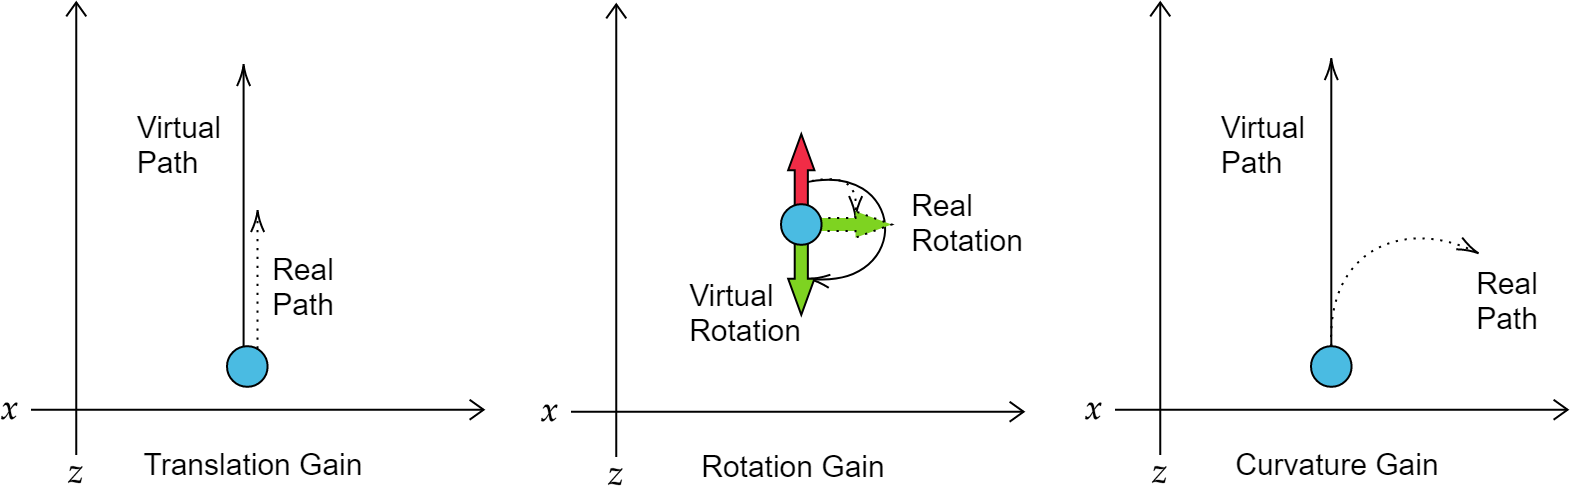
\includegraphics[width=1.0\textwidth]{figures/graphs/redirectionGains.png}
    \caption[Illustrated Example of How Redirection Gains Function]{This illustrated example shows how the three primary gains in redirected walking function.}
    \label{fig:redirectionGainsExample}
\end{figure}

Further illustration on how the different gains work can be seen in Figure~\ref{fig:redirectionGainsExample}.

Detection thresholds allow for the estimation of gains that can be applied without the user noticing them. As such, it has become a core of many other studies in the field. The taxonomy itself has since been extended by Suma et al.~\cite{suma2012taxonomy} to provide a more comprehensive look into additional redirection techniques. Outside of the three established redirection gains, an additional fourth type has recently been proposed by Langbehn et al.~\cite{7833190}. Their study presents the concept of bending gains which are similar to curvature gains but only applied whenever the user walks on a curve in the virtual world. 

In terms of relevance to research questions, the estimation of detection thresholds is directly relevant to $RQ_1$ as it provides a means to find undetectable gains. Despite this, there are some problems with this method of estimation that make it rather unsuitable to use. These are further mentioned in Section~\ref{sec:distractorUsageInLiterature}.

\subsection{Background: Redirection Algorithms}
In order to redirect a user, it is necessary to have a redirection algorithm. There are a variety of different redirection algorithms, but the two most common and generalised ones are as follows:
\begin{description}
    \item["Steer-to-Center"(S2C): ] A redirection algorithm that aims to steer the user towards the centre of the physical tracking space.
    \item["Steer-to-Orbit"(S2O): ] A redirection algorithm that aims to steer the user so they walk on the edge of a circle that encompasses the physical tracking space.
\end{description}
Both of these algorithms were originally presented by Razzaque~\cite{razzaque2005redirected} and have since been improved by Hodgson et al.~\cite{hodgson2013comparing}. The basis for these algorithms is to make use of rotation, curvature and translation gains in a manner that steers the user towards a desired point or direction. Among the two algorithms, S2C is generally believed to have the best performance, but S2O can perform better when long straight paths are travelled~\cite{hodgson2013comparing}. S2C has also been demonstrated to work particularly well for smaller physical spaces which is common for most virtual reality consumers today~\cite{azmandian2015physical}. 

Among the various redirection algorithms that exist, the most relevant for this thesis is Peck et al.'s "Improved Redirection with Distractors (IRD)"~\cite{peck2010improved}. This algorithm is an extension of the S2C algorithm with one primary addition: it makes use of virtual distractors to reorient the user towards the centre of the physical space when approaching physical walls. The usage of virtual distractors in redirected walking is further detailed in Section~\ref{sec:relatedDistractors}.

\subsection{Variables That Could Affect Redirected Walking and Detection Thresholds}
One thing to note about detection thresholds and the efficiency of redirected walking is that there are a variety of variables that can impact these. All the potential variables that were found throughout the sample of literature can be found in Table~\ref{table:DTVariables}. Since each variable is only briefly presented, there is a fair amount of abbreviated and potentially new terminology in use. The usage of abbreviated terminology will also increase from this point onwards in the thesis. As such, a short description of these can be found in Appendix~\ref{app:terminology} for quick referencing.

\begin{table}[!h]
\centering
\begin{tabularx}{\textwidth}{|m{2cm}|m{1.7cm}|m{10.1cm}|} 
\hline
\textbf{Variable} & \textbf{Research Discussing Variable} & \textbf{Research Results|Comments in Parentheses}\\
\hline
\hline
Size + Shape of Physical Tracking Space & 
\cite{azmandian2015physical} & 
There is no single ''optimal'' size.\newline Square shaped tracking spaces are the best choice for S2C and S2O algorithms.\newline S2C performs best in tracking spaces under 15m x 15m.\\
\hline
Optical Flow / Visual Density in VE & ~\cite{8446225, steinicke2008moving, 8446216, waldow2018textures} & Virtual environment size has no significant effect on detection thresholds.\newline It appears that low visual density/optical flow could make it harder to notice redirection.\newline Textures and global illumination have no significant effect on translation gain noticeability.\\
\hline
Hardware: HMD Field of View &
~\cite{fuglestad2018redirected}\newline Potentially relevant:\newline\cite{norouzi2018assessing} &
Detection thresholds for rotation and translation gain application are significantly lower with modern day hardware.\newline This could be caused by an increase in HMD field of view.\newline(This might correlate with increased optical flow).\\
\hline
Speed of Walking & \cite{5759454} & Likelihood of detecting curvature gains is significantly lower when walking slower.\newline Dynamic curvature gains allow for larger travel distances between resets compared to static gains.\\
\hline
Engagement / Distraction & \cite{5072212, schmitz2018you, sra2018vmotion}\newline Potentially relevant:\newline\cite{norouzi2018assessing, 5759454} & Whenever a user is engaged with a primary task or distracted by something, they appear to be less likely to notice that redirection is applied.\\
\hline
Awareness of Redirection & \cite{5072212} & If the user is not aware of the use of redirection, higher gains can be applied without being noticed.\\
\hline
Gender & \cite{nguyen2018individual} & Men seem to be more sensitive to curvature gains than women.\\
\hline
Adaptation: Curvature Gains & \cite{5072212, bolling2019shrinking, grechkin2016revisiting} & Exposing users to curvature gains for 20 minutes makes it harder to detect the gain. Similar effects might be possible for rotation, translation and bending gains. Gradually increasing the strength of curvature gains appears to cause some adaptation.\\
\hline
\end{tabularx}
\caption[Variables That Can Affect Detection Thresholds in Redirected Walking]{Variables that can affect detection thresholds in redirected walking.}
\label{table:DTVariables}
\end{table}

The variables that are found in Table~\ref{table:DTVariables} are relevant to this thesis as they can be used to inform the design of the virtual test environment, the use of redirection algorithms depending on available physical space and how to potentially maximise undetectable gains. Furthermore, the study by Azmandian et al.~\cite{azmandian2015physical} provides a means to measure the quality of redirection which is relevant for $RQ_2$.

\subsection{Comfort and Cybersickness}
While redirected walking aims at optimising the use of available tracking space and still leverage the benefits of real walking, it can result in some problems. High redirection gains tend to result in cybersickness, which can be seen as a form of motion sickness~\cite{mousavi2013review}. In doing so, one of the primary benefits of real walking is lost. Ideally, the increase in cybersickness from redirected walking should be minimised to provide the best user experience while still efficiently using the tracked space. In relation to detection thresholds, Fuglestad's research has shown that there might be an additional threshold between noticeable redirection and increases in cybersickness~\cite{fuglestad2018redirected}. These insights mean that it could be feasible to use estimated detection threshold values for redirection with limited risk of cybersickness increases, even if the user notices it at times. Similar results have been found by Rietzler et al.~\cite{rietzler2018rethinking}, suggesting that the use of curvature gains can be noticeable, but still acceptable. 

Outside of high redirection gains, there are also other factors that could increase cybersickness or limit user comfort. Dynamic field of view has for example been shown to potentially increase cybersickness~\cite{norouzi2018assessing}. Women might also be slightly more susceptible to cybersickness than men due to a slightly larger field of view~\cite{hildebrandt2018get}. Newer results from Nguyen et al. suggest otherwise though, as no significant increase in simulator sickness was found between genders in one of their experiments~\cite{nguyen2018individual}.

Due to the potential negative implications of standard redirected walking techniques, some researchers have developed new means of redirection. Suma et al. have made use of change blindness as a way to redirect without any type of gains~\cite{suma2011leveraging}. Despite this, their method only works for indoor environments and requires additional engineering for each individual room amongst these. Sra et al. have made use of scene rotation whenever the user is engaged with a task to leverage inattentional blindness~\cite{sra2018vmotion}, but their approach only works with predefined paths. 

From the point of view of a virtual environment designer, it would not be ideal to impose too many restrictions on how the environment is designed. At the same time, it is crucial to consider that cybersickness should be minimised as much as possible. Not doing so, can result in some ethical ramifications which are discussed in Section~\ref{sec:ethics}. For this thesis in particular, it is helpful to know that cybersickness can exist at a higher threshold than detection as this means that estimated gains could be possible to use safely. This knowledge has also been used to inform the method for estimating detection thresholds. 

\subsection{Subjective Sense of Presence}
Subjective sense of presence is a central part of virtual reality experiences. By properly immersing the user into a virtual world, it is possible to provide an engaging user experience. Subjective sense of presence can be negatively affected by a variety of techniques in redirected walking, which can compromise the overall experience of the user. 

The first of these are high redirection gains. Similar to Fuglestad's research that shows a difference between noticeability and cybersickness thresholds~\cite{fuglestad2018redirected}, Schmitz et al. presented that presence/immersion breaks at a different threshold from detection~\cite{schmitz2018you}. This insight means that certain gains of redirection can be noticed without resulting in cybersickness increases or breaks in presence.
Outside of redirection gains, another technique that can affect the subjective sense of presence is forced reorientation/resetting. Resetting techniques are fail-safes that are used whenever the user starts to exit the physical tracked space due to insufficient redirection~\cite{williams2007exploring}. An example of this would be to instruct the user to stop and rotate 360 degrees in the virtual world while they only rotate 180 degrees in reality due to applied rotational gains~\cite{suma2012taxonomy}. By doing so, the user is reoriented so that they no longer are in danger of leaving the tracked space. The problem with these types of techniques is that they are very intrusive and easily break any subjective sense of presence as users have to temporarily stop their in-game activity prior to resetting. 

Azmandian et al. mention that the average user should expect to have a physical tracking space that is 10m x 10m or lower, which results in many resets as unnoticeable redirection is not sufficient~\cite{azmandian2015physical}. Therefore, they suggest that the focus should be on improving existing reset/reorientation mechanisms and improving integration into the experience to limit breaks in presence. Improved subjective sense of presence and improved redirection are among the main areas that distractors aim to improve~\cite{peck2009evaluation, peck2011evaluation} which are the focus of this thesis.

\section{Distractors in Redirected Walking}\label{sec:relatedDistractors}
Distractors in redirected walking were originally presented by Peck et al. in 2009~\cite{peck2009evaluation}. In their study, the participants were instructed to watch a moving sphere and use this ''distraction'' as a means to increase redirection. Since then, various researchers have further improved distractors, although the term itself has acquired a few different semantic meanings. At the simplest level, a distractor when employed with redirected walking, aims to occupy the user's attention so that it is harder to notice redirection. As such, it is also possible to increase redirection during distraction~\cite{5072212}. This effect could potentially be a result of inattentional blindness which Sra et al. mention in their study on distractors~\cite{sra2018vmotion}. Distractors are triggered in a similar way to previous reorientation techniques (often shortened to "ROT", "ROTs" or simply resets), meaning that they activate whenever the user moves towards the edge of the physical tracking space. Compared to previous ROTs, distractors activate at a lower distance from the centre which means that existing ROTs can still be used as a fail-safe if the distractor itself fails to redirect the user~\cite{suma2012taxonomy}. Results from previous research also suggest that distractors result in higher levels of subjective presence compared to previous ROTs~\cite{peck2011evaluation}. 

From the acquired sample of literature, it does not seem that there is any formal taxonomy that defines the elements of distractors or their types. The closest to this would be Suma et al.'s taxonomy on redirection techniques~\cite{suma2012taxonomy}, but this taxonomy is too general to specify the details for distractors. As such, a grounded theory approach~\cite{strauss1994grounded} has been used to generate a taxonomy that classifies the most apparent elements that distractors consist of. This taxonomy will also be used as a framework to review the acquired sample of literature on distractors.

\subsection{Taxonomy of Distractors in Redirected Walking}\label{sec:distractorTaxonomy}
In cinematic VR, a similar topic to distractors is guided attention. While the goals behind a distractor and guided attention are somewhat different, there is some overlap that could be useful to consider. Taking inspiration from the taxonomy on redirected walking by Suma et al.~\cite{suma2012taxonomy}, Nielsen et al. have created a taxonomy of cues for guiding user attention in VR~\cite{nielsen2016missing}. Their taxonomy consists of three dimensions: explicit/implicit cues, diegetic/non-diegetic cues and whether they limit the ability to interact with the virtual environment (shortened to VE). Limiting interaction in the VE is not quite as relevant for redirected walking with distractors as physical walking is required, but the other two dimensions have been adapted into this taxonomy. The following sections describe general elements that can apply to any distractors, a distinction between two types of distractors and some elements that one of these can consist of. 
\subsubsection{Explicitness}
One of the relevant elements from Nielsen et al.'s taxonomy is explicitness. This element is split into explicit and implicit cues. An explicit cue consists of communicating that an event or object is deserving of attention while an implicit cue is meant to guide attention by simply being salient or interesting. In terms of distractors, these can also be explicit or implicit. An example of an explicit distractor would be a moving enemy in a VR game or something that the user has been told to pay attention to whenever it appears. As long as the user is told that they should pay attention to something, regardless of its purpose in the VE we can consider it as an explicit distractor. 

Implicit distractors on the other hand, would be distractors that can catch the user's attention in an almost instinctive manner. These could be salient elements that pop up in the peripheral vision of the user, potentially making them turn their head to see what it is. Another example would be a firefly that flies around and could catch the user's attention simply due to its salience in a darker environment. Compared to an explicit distractor like an enemy that the user knows they have to defeat, implicit distractors do not explicitly communicate how the user should react or interact with them. 

Currently, the usage of distractors is mostly of the explicit variety. A reason for this could be that the risk of ignoring an implicit distractor might be high. Unless the implicit distractor intrudes in a way that requires action from the user, it might not be seen as anything other than a detail in the scenery. The risk of ignoring a distractor can be problematic as there might not be enough redirection to avoid moving to the physical tracking boundaries. An effective implicit distractor might also be more challenging to design. It could be beneficial to have some background in psychology or neuroscience to understand what a natural user response would be to various implicit distractor scenarios.  

\subsubsection{Context Sensitivity}
An important aspect of distractors in the state of the art literature is context sensitivity~\cite{chen2017towards, chen2017supporting, sra2018vmotion}. Initial distractor implementations were fairly generic and worked similarly to standard ROTs, albeit with some changes. An example of this would be the hummingbird distractor from a study by Peck et al.~\cite{peck2011evaluation}. This distractor appears whenever the user approaches the physical boundaries and flies back and forth in front of the user. The user has in this case been instructed to keep their attention on the hummingbird, which then is exploited for redirection and reorientation. The downside of these generic types of distractors is that they serve no other purpose in the virtual experience other than to exploit the user for redirection and reorientation. This context insensitivity might not be ideal in terms of subjective sense of presence and can be seen as too repetitive if used too frequently. 

Instead, the focus with state of the art distractors has been to integrate them into the virtual experience so they serve additional purposes. VR games in particular are a good fit for integrating distractors as they can be included as game mechanics that are a central part of the experience. By doing so, there is less of a need for specialised instruction outside of understanding the premise of the game. There is also a belief by researchers that doing so will increase the subjective sense of presence~\cite{chen2017supporting, sra2018vmotion}. Improving the subjective sense of presence can be an important consideration in the design of distractors as they could improve the user experience. 

Based on what has been seen in the literature, distractors could be categorised within four types of context sensitivity: Insensitive, Visually Integrated, Mechanically Integrated and Fully Integrated (Both visually and mechanically).

\subsubsection{Distractor Types}
The term ''distractor'' has primarily been used to describe objects in the virtual environment (VE) that behave in a way that allows for redirection to be applied during distraction. A study by Sra et al.~\cite{sra2018vmotion} made use of distractor activities or simply ''attractors'' as they called it, which carries a slightly different semantic meaning. Due to this, it could be useful to differentiate between these two by splitting them into concrete and abstract categories.

\paragraph{Concrete Distractors}
If a distractor is an object or virtual existence in the VE, we can consider this as a concrete distractor. Concrete distractors consist of a variety of design elements which are further specified in the section following the description of abstract distractors. 

\paragraph{Abstract Distractors}
An activity on the other hand, can be considered as an abstract distractor. An activity can keep the user's attention by itself, but it can also consist of concrete distractors which require further attention of the user. If an abstract distractor is defined as an activity, then it is arguably explicit by nature as the user generally is aware of how they have to engage with it. An example of an abstract distractor would be to play a game, as various game elements and mechanics can keep the attention of the user. It does not matter what type of game the user plays as simply being engaged with it can be considered as a distraction, although its strength can of course vary. 

Abstract distractors can also be context sensitive or insensitive. An example of a context insensitive, abstract distractor would be to ask the user to perform a task that is entirely unrelated to what they are doing in the VE. An example of a context-sensitive, abstract distractor could be the activity of stargazing in an exploration-focused night-time scene. The activity of looking up into the sky could in this case allow for scene rotation while the user is looking upwards. The key to context sensitivity for these types of distractors is that they are believable and natural to the environment they are used in. 

\subsubsection{Elements of Concrete Distractors}
Concrete distractors can consist of a variety of elements that might result in specific user behaviour or to improve the user experience. The following paragraphs discuss the most apparent elements that were found by reading through the acquired sample of literature on distractors. This part of the taxonomy should be very easily extendable so that additional elements can be added in future work. 

\paragraph{Diegetic/Non-diegetic Existence}
The second element from Nielsen et al.'s framework regarding diegetic/non-diegetic cues is mostly relevant to concrete distractors. They define a diegetic cue as a cue that is a part of the world in the VE. By being part of the world, these cues are not only visible to one user, but also to any other users or computer controlled characters. An example of this would be to have a nearby volcano erupt. This event is then noticeable by both the players and any potential virtual characters in the narrative. A non-diegetic cue on the other hand, is only visible to one user. An example of this would be a HUD or GUI that only one user sees. To provide some examples within the scope of concrete distractors: a concrete, diegetic distractor could be a virtual character that the player interacts with while a concrete, non-diegetic distractor could be useful information in a HUD that the player wants to frequently keep attention on.

Diegetic cues could potentially improve the subjective sense of presence as Nielsen et al. achieved borderline significant results in their study~\cite{nielsen2016missing}. This insight could in turn also be relevant for concrete distractors. At the same time, in the context of games, it is not uncommon to have certain UI or elements that always are visible on the screen. If the game does not aim for realism, suspension of disbelief from the player could still result in a high subjective sense of presence. Due to this, one should not outright discredit the usage of distractors that are non-diegetic.

\paragraph{Movement}
Another element that concrete distractors consist of is movement or the lack of it. In terms of redirection, a concrete distractor can move around in a way makes the user turn their head. This movement can be used to apply rotational gains. An example of this would be a concrete distractor that orbits around the user and is important enough that they want to keep it in their vision at all times. If a concrete distractor moves towards the user, it might result in the user attempting to avoid it which can be used to move them away from physical walls or to apply redirection. A concrete distractor can also be useful for head-turning when static. An example would be to place a treasure chest at an angle from the user. In order to get the treasure, the user has to turn their head and move towards it which can be combined with rotation, curvature and translation gains.

\paragraph{First Appearance in Vision}
How the concrete distractor first appears in the user's vision is also something to consider. It could appear in plain sight, in the peripheral vision or outside of the user's vision. If a concrete distractor appears in the user's peripheral vision, it might catch their attention and make them turn their head to see what it is. If it appears outside of the user's vision, an audio cue or visual effects could be used to direct their attention towards where it is. If it appears in plain sight, the distractor might need to move around in order to apply rotational gains or to keep the user occupied so they do not notice a scene rotation. An example of this would be a merchant that allows the user to view their wares in a book or pamphlet. While the user is reading, the scene can rotate for the sake of redirection. 
         
\paragraph{Deterrents and Attractors}
Peck et al. introduced the concept of deterrents as a supplement to distractors~\cite{peck2011evaluation}. In their study, a deterrent was defined as something that deters the user from moving towards it. An example of a deterrent would be walls of fire that a fire-breathing dragon creates in Chen and Fuch's study~\cite{chen2017supporting}. In their study, these deterrents were used as a means to deter the user away from physical walls through strategic placement. Given that deterrents are capable of catching the user's attention, they could be seen as a type of concrete distractors. 

The opposite of a deterrent would be an attractor which the user wants to engage with. This definition is similar to Sra et al.'s definition of attractors~\cite{sra2018vmotion}, but instead of an activity, this definition is focused on concrete distractors. One of the previous examples of a treasure chest appearing at an angle that forces redirection could also be considered as an attractor. 

\paragraph{Salience}
The final element of concrete distractors is salience. Salience is defined as how easily a visual object stands out from its surroundings. In terms of distractors, salience can be important so that the user can quickly identify and place their attention on any concrete distractors that are used. An example of salient things that are effective at drawing attention could be moving objects or moving lights~\cite{rothe2018guiding}. 
Visual salience is comprehensive enough to be its own topic, although Nielsen et al. have mentioned some central factors that are believed to influence salience~\cite{nielsen2016missing}:
\begin{itemize}
    \item Luminance Contrast
    \item Edge or Line Orientation
    \item Colour
    \item Motion
    \item Stereo Disparity
\end{itemize}
One thing to note about these factors is that it is also important to consider how they contrast with the surrounding environment. Furthermore, the distribution of salient regions in a scene has a significant impact on how the user explores it as seen in a study by Sitzmann et al.~\cite{sitzmann2018saliency}. Their findings show that having few salient regions in a scene results in attention being shifted faster towards anything salient. As an additional effect, this attention is also more concentrated. These insights have been considered in the design of the virtual experience that is used for Experiment 1 and 2 in this thesis.

\section{Usage of Distractors in the Literature}\label{sec:distractorUsageInLiterature}
The previously generated taxonomy has been used as a framework to map out the usage of distractors in the acquired sample of literature. This mapping can be found in Table~\ref{table:DistractorsInLiterature}.

\begin{sidewaystable}[p!]
\centering
\scalebox{0.8}{
\begin{tabularx}{\textwidth}{|m{2cm}|m{1.5cm}|m{2cm}|m{1.9cm}|m{2cm}|m{7.55cm}|} 
\hline
\textbf{Distractor} & \textbf{Used in Study} & \textbf{Explicitness} & \textbf{Context Sensitivity} & \textbf{Distractor Type} & \textbf{Additional Relevant Elements}\\
\hline
\hline
Floating Sphere & \cite{peck2009evaluation} & Explicit & Insensitive & Concrete & Non-diegetic, Has movement, Appears in front of user.\\
\hline
Butterfly & \cite{peck2009evaluation, norouzi2018assessing} & Explicit & Insensitive: \cite{peck2009evaluation},\newline Visually Integrated: \cite{norouzi2018assessing} & Concrete & Diegetic, Has Movement.\\
\hline
Ghost & \cite{peck2010improved} & Explicit & Visually\newline Integrated & Concrete & Diegetic, Has Movement, Appears in front of user.\\
\hline
Hummingbird & \cite{peck2011evaluation, suma2012taxonomy} & Explicit & Insensitive & Concrete & Diegetic, Has Movement, Appears in front of user.\\
\hline
Horizontal Bars & \cite{peck2011evaluation} & Implicit & Fully\newline Integrated & Concrete & Diegetic, Static, Fades into view as user nears physical walls, Used as a deterrent.\\
\hline
Temporary Objectives & \cite{grechkin2015towards} & Explicit & Undefined & Abstract & None.\\
\hline
Moving NPCs & \cite{5759454} & Implicit & Fully\newline Integrated & Concrete & Diegetic, Has movement, Moves into view from the side or walks in front of the user, Used as a deterrent.\\
\hline
Flying Dragon & \cite{chen2017towards, chen2017supporting} & Explicit & Fully\newline Integrated & Concrete & Diegetic, Has movement, Moves towards user from current position when active, Can be considered as a attractor.\\
\hline
Flame Walls & \cite{chen2017towards, chen2017supporting} & Implicit & Fully\newline Integrated & Concrete & Diegetic, Static, Spawned by dragon when near physical walls, Used as a deterrent.\\
\hline
Watching Exotic Birds & \cite{sra2018vmotion} & Explicit & Fully\newline Integrated & Abstract & The activity itself consists of concrete distractors (birds). These birds move across the sky and have to be viewed through a pair of binoculars.\\
\hline
Observing Insects & \cite{sra2018vmotion} & Explicit & Fully\newline Integrated & Abstract & The activity itself consists of concrete distractors (insects). Among the many insects, the user is asked to keep one of them in focus.\\
\hline
Observing Insect in a Piece of Amber & \cite{sra2018vmotion} & Explicit & Fully\newline Integrated & Abstract & The user has to hold a piece of amber towards the sky and rotate so they can find a viewing angle that allows them to see the insect inside.\\
\hline
Interacting with NPCs & \cite{sra2018vmotion} & Explicit & Fully\newline Integrated & Abstract & The user has to hold a conversation with a NPC which acts as a concrete distractor.\\
\hline
Playing a target shooting minigame & \cite{fuglestad2018redirected} & Explicit & Fully Integrated & Abstract & The targets that move around could be considered as concrete distractors. \\
\hline
\end{tabularx}}
\caption[Distractors in Literature, Framed Within ''The Taxonomy of Distractors in Redirected Walking'']{List of all distractors that were used in the sample of literature, framed within the ''The Taxonomy of Distractors in Redirected Walking''.}
\label{table:DistractorsInLiterature}
\end{sidewaystable}
When looking at the current usage of distractors from the sample of literature, a few insights can be gained. Most distractors are explicit and the only instances that could be regarded as implicit were in cases of deterrents. Due to this, there are potentially unexplored areas when it comes to designing implicit distractors. As already mentioned in the description of the taxonomy, these can be rather challenging to design which is why we might not see them being used very often. Despite this, recent developments into redirected walking with eye tracking hardware makes use of techniques that closely resemble implicit distractors and could arguably be categorised among these. Some additional information on this can be found in the following section.

All of the concrete distractors in this review were also diegetic. This means that there is room to explore non-diegetic, concrete distractors that are integrated into the experience. Non-diegetic distractors could for example be used as aids for the user in games or scenarios where extra contextual information is helpful. 

Outside of the previously discussed elements, it should be noted that initial forms of distractors were mostly insensitive to context and could be seen as relatively generic. Over time, distractors have started to become more visually integrated with their respective virtual environments. The current state of the art has focused on fully integrating distractors by combining them with game mechanics and activities. Even so, the integration could go further as the currently developed prototypes are very simple. This thesis has aimed to develop a game prototype with a slightly broader scope than existing work and fully integrate it with distractors. The overall design space of fully integrated distractors is relatively large, which allows for additional exploration by researchers. There is not much documentation on the effectiveness of these types of distractors either, creating an opportunity for new research in the area~\cite{nilsson201815}. This thesis aims to provide some documentation on this through an experiment related to $RQ_2$.

The significant focus on context sensitivity in the field of distractors does create somewhat of a mismatch with the rigid structure of Steinicke et al.'s detection threshold estimation procedure~\cite{5072212} though. In particular, it becomes hard to create a virtual experience where distractors are fully integrated as the method for estimating detection thresholds would interfere too much with the possible design space of the experience. This issue is further coupled with some ethical problems which are discussed in Section~\ref{sec:ethics}. In the end, these issues makes it hard to justify using the standard procedure for estimating detection thresholds. As such, an alternative procedure is employed which is detailed in Section~\ref{sec:ex1EstimationMethod}. 

\section{Eye Tracking in Redirected Walking: A New Use Case For Distractors}\label{sec:relatedEyeTracking}
A sub-field within redirected walking that recently has seen some major development is the employment of eye tracking hardware to further redirect users. Sun et al. have created a redirection system that performs small redirections during eye saccades, which consist of a small moment of temporary blindness~\cite{sun2018towards}. Furthermore, they make use of a subtle gaze direction method which adds additional salience to nearby objects or elements in the environment that are in the peripheral vision. As a result, this implicitly encourages the eye to move towards these regions. This technique could very well be framed as using implicit distractors from the previously presented taxonomy and provides an interesting use case for distractors. By combining distractors with state of the art redirection methods that use eye tracking, it could be possible to further improve the potential strength of redirection. As distractors are aimed at keeping user attention, they would be very well fit to help with triggering eye saccades, particularly so if they move around. 

Outside of Sun et al.'s study, Langbehn et al. have introduced a similar technique that instead exploits eye blinks as a means to perform small redirections~\cite{langbehn2018blink}. As part of their suggestions for how to increase the amount of eye blinks a user makes, they suggested making use of bright lights or virtual objects that move towards the eye of the user. This suggestion could also be seen as a use case for distractors. As a result, if accurate and effective eye tracking hardware ends up becoming more common in the future, we might see distractors become an essential building block of future redirection techniques with this technology. 

For this thesis, making use of eye tracking hardware is outside of the scope. There are a few reasons for this. First of all, while VR eye tracking hardware is available for experimentation at campus, the accuracy of the tracking drops during moderately fast head turns. This accuracy issue is problematic when using distractors as they may result in fast head turns. The reason for this accuracy drop in general is that the eye tracking hardware is calibrated with the assumption that the head-mounted display (HMD) stays static on the user's head. If a user then moves their head so the HMD receives even a tiny displacement in its position, the calibration starts to become inaccurate. This displacement could for example pose a problem for detecting eye saccades, while this would likely be less of an issue for detecting eye blinks. 

Furthermore, the addition of eye tracking hardware would introduce an additional variable to an already complex experimental environment. Given the already large scope and complexity of this environment, it would be preferable to limit any additional confounding factors. Employing eye tracking hardware would also require individual calibration per experiment participant. This calibration would result in additional overhead, which could take too much time away from other experiment components. 

\section{External Validity of Estimated Detection Thresholds}
Given the number of variables that potentially could affect detection thresholds, it would be difficult to think of these as generalised thresholds. For example, the thresholds that Steinicke et al. initially estimated were thought of as a worst case scenario due to the isolated nature of the study~\cite{5072212}. As such, they should be considered as a baseline while higher redirection is possible due to a variety of variables like engagement or distraction. Despite this, Fuglestad's results have shown that this baseline might be significantly lower than that of Steinicke et al.'s estimations due to the potential effect of better hardware~\cite{fuglestad2018redirected}. As such, one might start to wonder what role detection thresholds can fulfil as their generalisability is limited by many factors.  

Despite this limitation, there are still a variety of use cases that the estimation of detection thresholds could be applicable for. One of these would be as a tool to measure how much a variable can affect noticeability. By estimating baseline thresholds for a virtual experience and estimating a second group of thresholds whenever a variable is introduced or active, we can make direct comparisons in how the detection of redirection changes. As long as the context of the estimations is taken into account, detection thresholds can also provide a ballpark estimate for the expected amount of unnoticeable redirection. Given that similar contexts are employed by others, they should also receive similar results. If large volumes of detection thresholds were to be estimated across many different contexts and virtual environments, they might also help with providing an overview of the degrees which various variables can affect noticeability. 

This discussion is primarily relevant to $RQ_1$ and the estimation of detection thresholds. In particular, this research makes use of the first example when discussing use cases for detection thresholds where two groups of thresholds are estimated in one experiment. The first group consists of baseline detection thresholds for the virtual experience when no concrete distractors are active, while the second includes detection thresholds for when a concrete distractor is active. This approach allows for direct comparisons on how the introduction of concrete distractors changes the noticeability of redirection. This method of comparison does come with one caveat though. Estimating two groups of detection thresholds in the same amount of time as one would estimate one group results in lower accuracy. Despite this, as detection thresholds in general cannot be taken as entirely accurate due to the number of variables that can potentially affect the result, some error should be acceptable. 

\subsection{Use of Informed/Uninformed Participants for Redirection}
Among the various variables that can affect the noticeability of redirection, awareness of redirection could need some additional discussion. Steinicke et al. mention in their study on detection thresholds that it was possible to increase unnoticeable redirection when the user is unaware of it~\cite{5072212}. This unawareness has since been part of various experiments within redirected walking. For example, all the current state of the art studies on distractors did not inform their participants of redirection before the experiment~\cite{sra2018vmotion, chen2017towards, chen2017supporting}. While this can provide higher unnoticeable gains, one important question to think of is how applicable this would be in the real world. 

If we think of a real-world scenario where a successful application or game makes use of redirected walking, would it be realistic to assume that every single user is unaware of redirection? Since we live in a day and age where the internet keeps us connected, if some users discover the employment of redirection, this information can quickly spread to many others. This spread of knowledge could in turn result in the redirection becoming more easily noticeable. At the same time, Steinicke et al. also mention that being engaged in primary tasks or activities have a similar effect~\cite{5072212}. If a user then knows of the redirection but is engaged enough into the virtual experience, it might help to counteract the otherwise increased noticeability. Of course, it would not be realistic to assume that all users know that redirection is used either as reality would most likely be somewhere in-between. 
 
The challenge lies in trying to design experiments that are closer to what we would expect in the real world. Informing participants to some degree is for example necessary when estimating detection thresholds as they should understand when they should report a detection. If the detection threshold gains are then used in a second experiment to test the performance of redirection, using uninformed participants would not change any results as the gains stay static. As such, for this thesis in particular, it would make the most sense to keep participants informed on redirection for all experiments. This thesis tries to move towards a middle ground between fully informed and uninformed participants. Instead of explicitly mentioning every detail relating to what redirection techniques that are used, participants are mostly given a brief introduction to the topic. They are then asked to notify whenever they detect that the virtual experience feels inconsistent or sluggish. Furthermore, a small amount of deceit is used by mentioning a few additional quality metrics to limit potential priming effects. The information and consent sheet that is given to participants can be found in Appendix~\ref{app:informationconsent}.

An additional benefit of not making use of fully uninformed participants is that the potential sample broadens as some participants could be reused between experiments. As already mentioned in the previous section, it is vital to consider the context of the estimated detection thresholds when looking at the results. To help with this, the context relative to the currently established variables is summarised when presenting the results in Chapter~\ref{chap:ex1}. 

\section{Ethics of Estimating Detection Thresholds}\label{sec:ethics}
One problem with researching redirected walking is the ethics around potentially causing cybersickness for participants. This can be particularly problematic when estimating detection thresholds with standard methods like Steinicke et al. have used~\cite{5072212}. Their method for estimating detection thresholds makes use of a two-alternative forced choice task with a uniform distribution of gains in a given range. These gains are then tested in random order where the participant has to answer whether the current gains are higher or lower than the norm. The problem with this approach is that this range of gains could have values that are high or low enough to result in cybersickness. As such, it could be considered to be unethical to estimate detection thresholds like this. Instead, this thesis makes use of an alternative method which is presented in Section~\ref{sec:ex1EstimationMethod}.

Another thing that should be noted is that all participants throughout the experiments in this thesis were told to stop the experiment at once if they experienced any cybersickness or nausea. While prematurely ending the experiment with a participant does not provide entirely accurate data, it can still hold some value for analysis. 
   
\section{Accessibility of Redirected Walking to Virtual Reality Developers}
If a developer is interested in or wants to test redirection techniques, they may be met with a relatively sizeable theoretical bar of entry. This bar of entry is mostly a result of the knowledge around redirected walking primarily being in the academic sphere with very few practical tutorials or code examples for how redirection techniques can be implemented. The possibility of having several key articles locked behind pay-walls does not help with this either. 

Despite this, there are some publicly available code repositories that can be looked at. A link to Fuglestad's implementation of various redirected walking elements in the Unreal Engine can for example be found in his masters thesis~\cite{fuglestad2018redirected}. Azmandian et al. have developed a redirected walking toolkit for the Unity Engine which consists of implementations for the S2C and S2O algorithms as well as some basic reset techniques~\cite{azmandian2016redirected}. It should be noted that this toolkit has not received any updates or additional features since its release in 2016. The work done with this thesis verifies that the toolkit is working with Unity's 2018.3 version.

The Redirected Walking Toolkit by Azmandian et al. is used as a base for implementation in this thesis. This choice is primarily a result of the author's preexisting familiarity with the Unity Engine, which allowed for a faster development process.

\section{Choosing a Sufficient Reset Technique}\label{sec:choosingTheRightReset}
One important thing to consider when developing a virtual reality experience that makes use of redirected walking is the reset technique that will be used. It should not be expected that redirection will be able to fully steer a user away from walls at all times, hence the necessity of these fail-safes. Regardless, there are quite a few different reset techniques available, potentially making it a challenge to choose the right one. 

There are three standard reset techniques which were initially presented by Williams et al.~\cite{williams2007exploring}:
\begin{description}
    \item["Freeze - Backup": ] The user is notified that they have reached the physical bounds and their virtual position is frozen. They are instructed to take steps backwards until the experience is unfrozen. 
    \item["Freeze - Turn": ] The user is notified that they have reached the physical bounds and the HMD display is frozen. They are instructed to turn 180 degrees, after which the display is unfrozen. 
    \item["2:1 - Turn": ] The user is notified that they have reached the physical bounds. They are instructed to turn 360 degrees virtually while a rotation gain of 2 is applied. This rotation results in a 360-degree turn in the virtual world and 180 in the real world.
\end{description}

Among these three, the 2:1 Turn technique is most commonly seen. This popularity could be due to its relative simplicity and what could be considered as a lower degree of intrusiveness compared to its alternatives. Freeze - Turn and Backup might also be seen as too jarring for users as they directly remove some control in terms of head and body movement in the virtual world.

While the 2:1 Turn technique is the most commonly used one, it does come with a few problems of its own. The high gain value of 2 could for example become uncomfortable for participants even if it only stays active for a short while. Another issue is that it is possible to become stuck between two adjacent sides of a room that are close to the corners. This issue is illustrated in Figure~\ref{fig:2to1turnProblem} and results in the user moving back and forth with resets happening in perpetual succession.  

\begin{figure}[htbp]
  \centering
  \includesvg{figures/svgs/2to1turn.svg}
  \caption[Potential Problem With 2:1 Turn Resetting]{A potential problem that can occur when using the 2:1 Turn resetting technique. The blue circle denotes the user. The red and green arrows indicate the facing direction before and after resetting. The shaded area is the bounds for triggering the reset technique.}
  \label{fig:2to1turnProblem}
\end{figure}

To deal with this problem, Nguyen et al. have provided two alternative resetting techniques~\cite{nguyen2018discrete}:

\begin{description}
   \item["To Center": ] This resetting technique tells the user to rotate 360 degrees virtually. A gain value is precomputed so that the facing direction of the user ends up towards the centre of the tracked space once the rotation is finished. As a result, the user rotates 360 degrees + an additional angle to offset them towards the centre of the tracked space.
   \item["To Corner": ] This reset technique works similarly to the "To Center" technique but instead targets the furthest corner in the room. 
\end{description}

These resetting techniques were shown to provide significantly less resets in total over the 2:1 Turn technique in a simulated scenario. Despite this, the authors did not consider an important practical problem that their resetting techniques can result in with current day HMD's. This problem is related to the physical tethering that most modern HMD's still use today. When rotating over 360 degrees in the real world, the tethered cable can easily get tangled and the user will need to avoid wrapping themselves in it. This wrapping is less of an issue for the 2:1 Turn reset as the user only rotates 180 degrees in the real world. 

To mitigate the various problems and issues that current day resetting techniques consist of, this thesis has created a variation of the Freeze - Turn reset. This new reset, dubbed as ''Pause - Turn - Centre'' is detailed in Section~\ref{sec:pauseturncentre}.

\section{Overall Answers to Research Questions}
Since the generated taxonomy has partially operationalised various elements of distractors, it would be prudent to update the terminology of the research questions as well. 
The updated research questions are as follows: 
\begin{description}
   \item[$RQ_1$: ] How noticeable is redirected walking with fully integrated distractors in a playful virtual environment?
   \item[$RQ_2$: ] Given the highest unnoticeable gains, how effective is redirected walking with fully integrated distractors in a playful virtual environment?
\end{description}

The following two paragraphs summarise how the related work is relevant to the research questions.

\paragraph{$RQ_1$}
For the first research question, a variety of variables that can affect detection thresholds in redirected walking have been mentioned. These have been considered when designing the experiment and corresponding virtual experience. By focusing on an engaging experience designed around fully integrated distractors, it might be harder to notice the redirection, which in turn could allow for stronger gains. A method for measuring detection thresholds has also been provided by Steinicke et al.~\cite{5072212}, but it is not used due to problems related to ethics and generally not working well with the theme of fully integrated distractors. The current state of the art is focused on fully integrated distractors and the literature sample provided no research measuring detection thresholds for these. As such, measuring the detection thresholds for fully integrated distractors should be a reasonable contribution to the field of distractors in redirected walking.

\paragraph{$RQ_2$}
Azmandian et al. have provided a method to measure the effectiveness of redirection by recording the total number of forced reorientations using standard reset techniques~\cite{azmandian2015physical}. Since standard reset techniques can be included as fail-safes for distractors, this is relevant to make use of for this thesis. Furthermore, this method also allows for comparison with a control condition to find the relative increase in effectiveness.

Breaks in presence and cybersickness are thresholds that can exist at higher gains than detection. Due to this, it would be reasonable to focus on the highest unnoticeable gains as the risk of negative impact on the experience for participants should be minimal. 

\section{Usage of Distractors in Other VR Research Fields}
While distractors are just one sub-field of redirected walking, there are similar concepts used in other VR research fields as well. One of the already mentioned ones is using cues in cinematic VR as a means to guide the attention of the user towards areas of interest during watching~\cite{nielsen2016missing}. Another area where we can see the usage of distractors is in the medical field where they are used for pain relief~\cite{malloy2010effectiveness, knight2018virtual}. In this field, abstract distractors are used as a means to reduce the pain that patients experience under burn injury care or to reduce experimental pain~\cite{malloy2010effectiveness}. Furthermore, using VR distractions has shown to significantly decrease the amount of reactive pain behaviour in comparison to traditional distraction methods~\cite{knight2018virtual}. 

In general, we can see that the concept of distracting someone for either their own benefit or for entertainment can be employed in various ways in different fields of VR research.

\section{Background: Transformation Hierarchies in Game Engines}
As part of Chapter~\ref{chap:implementation}, there will be more technical implementation details on how the various redirected walking parts of the solution are implemented. In order to understand these technicalities as well as Azmandian et al.'s toolkit~\cite{azmandian2016redirected}, it is first necessary to provide some background on one important topic: Transformation hierarchies in game engines.

A transformation hierarchy in computer games is a relatively simple concept, but can result in rather complex behaviour. This hierarchy is a specific subset of functionality from a concept known as scene graphs, which used to logically couple together objects in a 3D scene. The gist of a transformation hierarchy is that objects or entities can be parented to each other. When parented, the child will no longer be positioned directly in world space, but rather relative to its parent. As such, if a parent moves, so will all of its corresponding children who may have individual relative positions within the hierarchy. This cascading effect does not only have to be in respect to position changes, but also scale and rotation. If we for example have a car object in a game with all the individual parts as children of a root node, then we can modify the position, rotation or scale of the root and it will propagate to each of the children. This way, we can rotate, re-position or scale the entire car by merely modifying the root node in the hierarchy.

\section{Background: The Redirected Walking Toolkit}
Since the implemented solution for this thesis makes use of the redirected walking toolkit~\cite{azmandian2016redirected} as a base, it is first necessary to at least have an overview of it. 

\subsection{How Redirected Walking is Implemented in the Toolkit}
An interesting side effect of transformation hierarchies is the perception of change for the child nodes. This effect is essential to how redirected walking is implemented in the redirected walking toolkit. To best illustrate this effect, it is easiest to provide an example. Consider that we have a parent: \textbf{''Redirection Root''} with two children \textbf{''Camera''} and \textbf{''Physical Space Representation''}. The camera can move around in the representation of physical space and both children will always be correctly mapped with each other, regardless of how the parent's transformation changes. As children, from their perceived point of view, they are consistent with each other due to how transformation hierarchies function. The interesting part becomes if we place our virtual world outside of hierarchy that the root governs, or rather have root and virtual world on the same hierarchical level. 

If we now rotate the redirection root, the children will have the perception that it is the virtual world itself that rotates, and not themselves. Despite what the children perceive, it is their redirection root parent that rotates and not the virtual world itself. This effect is the essence of how redirected walking is implemented in this case. Both curvature and rotation gains are implemented by injecting small amounts of rotation to the y-axis of the redirection root as the child camera moves and looks around. By doing so, it is possible to create the perceived effect that the child camera rotates more or less in the virtual world, compared to the real one. In a similar vein, it is possible to create curved paths. 

\subsection{Toolkit Terminology}
The toolkit uses slightly different semantics and terminology compared to what we could consider as the standard set by Steinicke et al.~\cite{5072212}. For the sake of consistency with the toolkit itself, this terminology will be used forwards in the thesis. The terminology that is different and their equivalents are as follows:

\subsubsection{Rotation Gains}
The toolkit does not semantically think of rotation gains as a multiplier to head movement, but rather as a percentage increase or decrease which are respectively named positive and negative rotation gains. For example: a rotation gain multiplier of 2, meaning that head rotations are twice as fast in the virtual world would be the equivalent to a positive rotation gain of 1. In this case, it is a 100\% increase over the base rotation. A multiplier of 0 would respectively be equivalent to a negative rotation gain of -1, meaning that the head no longer can rotate on the y-axis.

\subsubsection{Curvature Gains}
Instead of defining curvature gains as a ratio relative to the radius of the circular arc, the redirected walking toolkit defines curvature gains as curvature radius. In this case, a curvature radius of 5m means that the user's curved path will be on the edge of a circle that has a radius of 5m. 

\subsubsection{Forced Reorientation Techniques}
''Forced reorientation techniques''/''ROTs'' are generally either called by this semantic name or simply as ''resets''. There is no direct consistency in the literature regarding which one researchers use, but the toolkit uses ''resets'' as the term for forced reorientation techniques. 

\subsection{Toolkit Structure}
\begin{figure}[tbph]
    \centering
    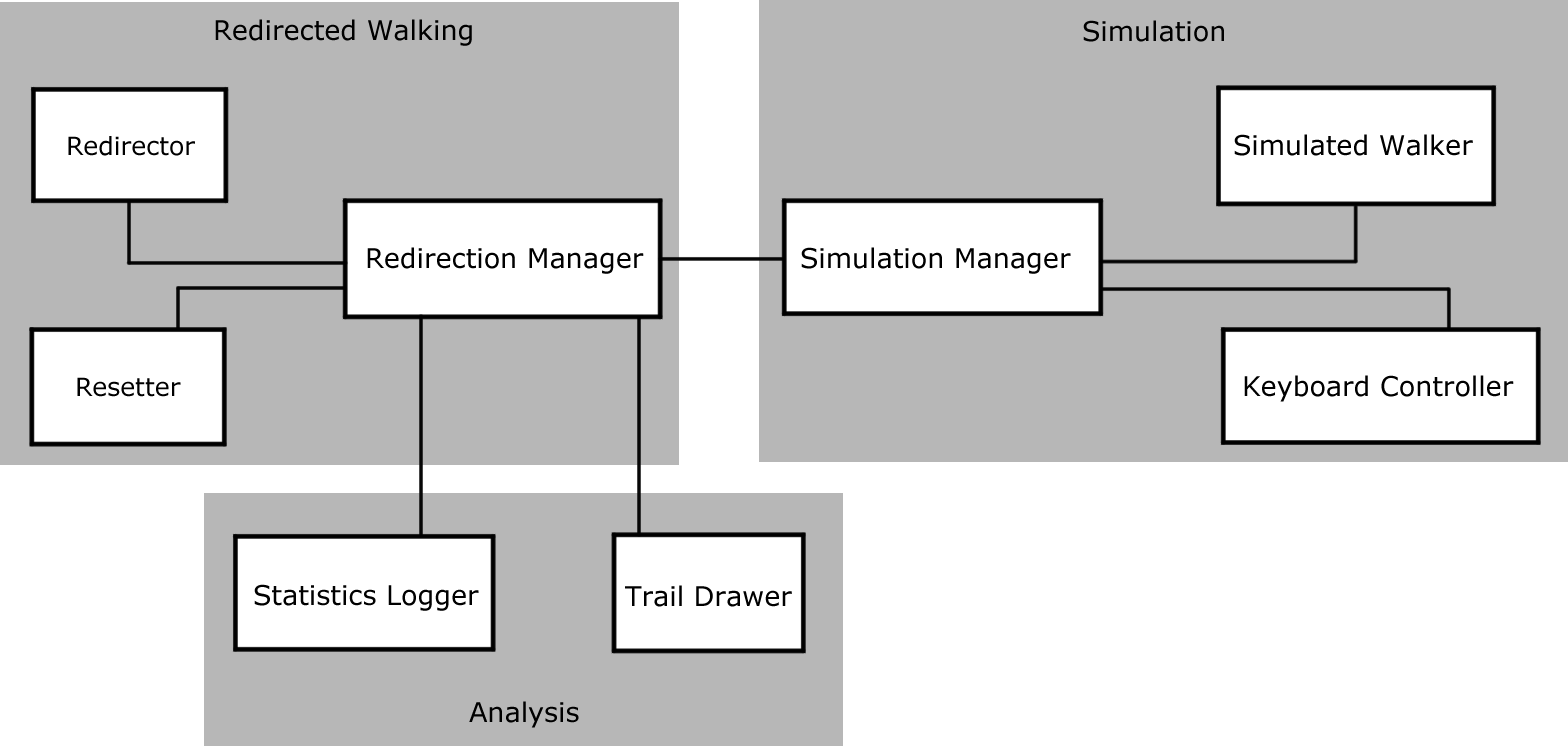
\includegraphics[width=1.0\textwidth]{figures/graphs/ToolkitStructure.png}
    \caption[Structure of the Redirected Walking Toolkit]{This illustration shows a recreation of Azmandian et al.'s figure~\cite{azmandian2016redirected} which gives an overview on the structure of the redirected walking toolkit. The structure has been further extended by the work in this thesis as discussed in Section~\ref{sec:extendedRDWToolkitArchitecture}. The extended structure can be seen in Figure~\ref{fig:rdwToolkitExtendedStructure}.}
    \label{fig:rdwToolkitStructure}
\end{figure}

The redirected walking toolkit's overall structure is divided into three parts. These can be seen in Figure~\ref{fig:rdwToolkitStructure} and consist of redirected walking, simulation and analysis components. The work in this thesis is primarily related to the redirected walking side of the toolkit and as such, this part will be further detailed. 

\subsubsection{RedirectionManager}
The main control point of the toolkit is the \lstinline{RedirectionManager} script. The script itself is attached to the root object in the redirected walking object hierarchy and as the name implies, manages the whole solution. This management includes keeping track of the strength of gains, calling virtual functions on redirectors and resetters when applicable, and facilitating general communication between all of the components in the toolkit. 

\subsubsection{Redirectors}
Redirectors are the scripts in the toolkit that manage the injection of camera angles which results in redirection. All redirectors have to extend a base \lstinline{Redirector} script which makes use of various virtual functions that are called as necessary by the \lstinline{RedirectionManager}. The S2C and S2O redirectors are examples of scripts that in this case extend the base redirector class. This class allows for a generic approach where any type of redirector could be developed as long as it complies with the structure and virtual functions of the base class. 

\subsubsection{Resetters}
Resetters are similarly structured to redirectors. A resetter is capable of the same functionality as a redirector, but is only active whenever the user leaves a defined safe area within the physical space. By default, a resetter is triggered whenever the user is 0.5m away from the edge of the physical space. Furthermore, a resetter has additional callbacks for when a reset has triggered and when it is finished to allow developers to easily work with these events. 

This concludes the background needed to understand the implementation details of Chapter~\ref{chap:implementation}. Before moving on to this chapter though, the general methods that were applied in this thesis are disclosed in the following chapter.
\chapter{General Methods} \label{chap:generalmethods}
This chapter consists of methods that are relevant to the thesis as a whole. Specific methods used for each of the two experiments can be found in Chapter~\ref{chap:ex1} and Chapter~\ref{chap:ex2}. 

\section{Literature Acquisition}
In order to find relevant literature for the literature analysis in Chapter~\ref{chap:relatedWork}, a variety of search terms and databases were used. The list of keywords, keyword combinations and literature databases that were used can be found in Table~\ref{table:literaturekeywords}. 
Similar searches were also conducted with the ACM digital library database, but these searches did not provide any additional literature that had not already been found in other searches. As such, these queries are not included in the table. As a side note, these queries are a refreshed and combined version of previous literature searches in the IMT4205 - Research Project Planning and IMT4894 - Advanced Project Work courses. 

\begin{table}[tbh!]
\centering
\begin{tabularx}{\textwidth}{|m{2cm}|m{1.7cm}|m{2.7cm}|m{1.5cm}|m{1.20cm}|m{3.375cm}|} 
\hline
Keywords & Database & Combination & Filter & Results & Chosen\newline for Reading\\ 
\hline
"Redirected Walking"\newline
"Threshold"\newline
"Thresholds"\newline
"Comfort"& Google Scholar & ("Redirected Walking") AND ("Threshold" OR "Thresholds") AND "Comfort" & After 2014 & 69 & 7\\ 
\hline
"Redirected Walking"\newline
"Threshold"\newline
"Thresholds" & Google Scholar & ("Redirected walking") AND ("Threshold" OR "Thresholds") & After 2018 & 119 & 6\\
\hline
"Redirected Walking"\newline
"Threshold"\newline
"Thresholds" & IEEEXplore & "Redirected walking" AND ("Threshold" OR "Thresholds") & None & 13 & 5\\ 
\hline
"Redirected Walking"\newline
"Distractor"\newline
"Distractors" & Google Scholar & ("Redirected walking") AND ("Distractor" OR "Distractors") & After 2016 & 76 & 3\\
\hline
"Redirected Walking"\newline
"Distractor"\newline
"Distractors" & Google Scholar & ("Redirected walking") AND ("Distractor" OR "Distractors") & None & 172 & 3\\
\hline
"Virtual Reality"\newline
"Distractors"\newline
"Redirection" & Google Scholar & ("Virtual Reality" AND "Distractors" AND "Redirection") & None & 186 & 3\\
\hline
"Cinematic VR"\newline
"Attention" & Google Scholar & ("Cinematic VR" AND "Attention") & None & 123 & 2\\
\hline
\end{tabularx}
\caption[Keywords and Combinations That Were Used for the Literature Search]{List over keywords and combinations that were used for the literature search.}
\label{table:literaturekeywords}
\end{table}

\subsubsection{General Literature on Redirected Walking and Detection Thresholds}
For the first three queries in Table~\ref{table:literaturekeywords}, literature was picked for reading as long as the title or abstract focused on either detection thresholds or user comfort. The focus of the queries was to find recent development within the field of redirected walking and the estimation of detection thresholds. All result pages were scanned through in these three queries. 

\subsubsection{Distractors and Attention}
Table~\ref{table:literaturekeywords} also consists of three queries related to distractors. The first of these was conducted to look for state of the art applications of distractors while the second and third were used to acquire background literature on the topic. For the first search, all pages of query results were scanned through. For the second and third searches, the first ten pages of results were scanned through due to the higher sample. 

One last query related to cinematic VR and attention was added to look for related work in this field. The ten first pages of results were scanned through for this query.
Literature was chosen for reading based on similar criteria as the queries in the previous section.

\subsubsection{Literature Acquired Through Citations}
As a secondary approach to acquiring literature, an additional \textbf{9} papers were found through citations in papers that were chosen in Table~\ref{table:literaturekeywords}. 

\subsubsection{Literature Acquired Through Discussions With Supervisors}
\textbf{3} additional research papers were acquired through discussions with the supervisors. These consisted of various research methodology papers as well as some pointers towards medical research that makes use of distractors in VR.

This puts the total amount of literature that was acquired at \textbf{41} papers for the literature review in Chapter~\ref{chap:relatedWork}.

\section{Personal Data Collection and GDPR Compliance}
Throughout the experiments, a demographic questionnaire was used to gather certain pieces of personal data. This section is dedicated to justify why each piece of personal data was collected and provide validation that the study itself is GDRP compliant. 

\subsection{Demographic Questionnaire}
The demographic questionnaire that was employed in both experiments can be found in Appendix~\ref{app:demographicsQuestionnaire}. It consisted of various demographical questions, as well as optional qualitative feedback questions. The reasoning for using the following demographical questions is as follows:

\begin{description}
   \item[Gender:] Given that there is prior research on the potential effects of gender on sensitivity to redirection~\cite{nguyen2018individual}, this is a relevant piece of data to collect. 
   \item[Age Range:] There may be cognitive differences between younger and older participants that can affect the result. Age ranges are used instead of direct age so that recognising individuals is more difficult. 
   \item[Whether the participant needed to remove any optical corrections while in VR:] If a participant needs to remove any optical corrections to make use of a VR HMD, the sharpness of their vision may or may not be compromised. This loss of sharpness could in turn have some effects on their sensitivity to redirection as it for example could affect the perceived optical flow. 
   \item[Whether the participant has taken part in prior redirected walking experiments:] This question was asked in case there are any trainable effects towards redirection. This could be the case as there may be similar effects to the possibility of mitigating cybersickness through training~\cite{hildebrandt2018get}. Furthermore, research suggests that adaptation effects exist for curvature gains~\cite{nguyen2018individual}.
   \item[How much prior VR experience the participants considers they have:] In a similar vein to the previous question, prior experience with VR could have some effect on how comfortable participants are in VR. This comfort level could in turn have some effects on how comfortable they are with using redirected walking.
\end{description}

One question that might have been relevant would be how much prior game experience participants have had. This question was not included in the questionnaire as research has suggested that this does not factor into the noticeability of redirection~\cite{nguyen2018individual}.

\subsection{GDPR Compliance and Data Anonymity}
In order to validate that this study was GDPR compliant and following other relevant regulations, an application form was sent to the Norwegian Centre for Research Data\footnote{\url{https://nsd.no/nsd/english/index.html}} (NSD). Their response, showing that the study is compliant with GDPR as well as their own terms, can be seen in Appendix~\ref{app:nsdApproval}. The following two paragraphs consist of a summary of the information that was provided in the application to NSD.

The demographic data that was gathered made use of a paper questionnaire and required written consent. These two were tied together with a numerical ID which could be used if necessary to remove any personal data if requested. Participants were asked at the end of each experiment if they wished to be given their ID so it could be used for GDPR related requests. The demographic data and written consent were stored in a securely locked box at campus until data processing was necessary. Once processing was necessary, the paper data was transcribed and stored on the author's private home directory at NTNU's servers\footnote{\url{https://innsida.ntnu.no/web/guest/wiki/-/wiki/English/Your+files+on+the+NTNU+server}}. This data was then processed using NTNU's software farm\footnote{\url{https://innsida.ntnu.no/wiki/-/wiki/English/software+farm}}. The demographical data on the private home directory as well as the paper information are planned to be destroyed on the thesis hand-in date.

Outside of the demographic information that was recorded, each of the two experiments recorded a variety of software side performance data. This data was also tied to the demographic information with a numerical ID, but stored in the project repository on GitHub~\cite{projectRepository}. This data is openly available as there is no way to tie it to any individuals without access to the demographic information.

\section{Development Environment}
The development environment that was used to develop the Ensemble Retriever VR game consists of: 

\begin{itemize}
    \item Unity Engine, version 2018.3.5f1.
    \item Microsoft Visual Studio 2017 Integrated Development Environment.
    \item SteamVR Unity plugin for virtual reality development.
    \item A Mersenne Twister library~\cite{MersenneTwisterLibraryLink} for cases where high-quality randomness is necessary.
    \item Azmandian et al.'s Redirected Walking Toolkit~\cite{azmandian2016redirected} for providing base redirected walking functionality.
    \item OpenVR Advanced Settings\footnote{\url{https://github.com/OpenVR-Advanced-Settings/OpenVR-AdvancedSettings}} to disable SteamVR's internal chaperone system.
\end{itemize}

Further details on Ensemble Retriever and additions to the redirected walking solution can be seen in Chapter~\ref{chap:implementation}.

\section{Hardware Environment for Experiments}
Throughout the two experiments, a desktop computer with the following specifications was used:
\begin{description}
   \item[CPU:] Intel i7-6700k
   \item[GPU:] Nvidia Geforce GTX 1080
   \item[RAM:] 16 GB
   \item[Operating System:] Windows 10 Pro
\end{description}

Together with this desktop computer, an HTC Vive HMD + Vive Controllers was employed together with 5m cable extensions to allow for full traversal of the physical tracking space without any significant tethering issues. The physical space that was used can be seen in Section~\ref{sec:ex1physicalRoom}. Finally, a pair of Audio Technica ATH-MSR7BK headphones were used to provide sound for participants. 

\section{Software Environment for Experiments}
On the software side, the developed Ensemble Retriever game was used while running in the Unity Editor. The reasoning for using the software in the editor rather than as a built version was that the employed version of Unity had build times that took several hours. This built approach would be rather inflexible in case any apparent issues appear during experiments that require rapid fixing. Instead, a more flexible option was used by running the game in the Unity Editor, allowing for small changes or fixes to be quickly implemented if needed. This approach does come with a small trade-off in terms of ingame performance as the editor results in higher overhead, but this was considered as a fair trade.  
\chapter{Implementation}
\label{chap:implementation}
\todo{lots of figures and screenshots should be used here}
\todo{Grammarly me}
This chapter consists of implementation details for all relevant redirected walking components as well as an overview of the game design for the developed ''Ensemble Retriever'' game. The game design overview is used to provide examples and documentation on how distractors have been fully integrated into the experience itself. 

\section{Open Source Repository - GitHub}
The source code and project assets for Ensemble Retriever can be found in a publicly available GitHub Repository~\cite{projectRepository}. It should be noted that the game itself is an extension of a small prototype that was previously developed for the IMT4894 - Advanced Project Work course. This prototype consisted of no redirected walking elements and simply featured a battle in VR against an angry contrabass enemy. The majority of the source code has needed to be rewritten or refactored to facilitate a more generic architecture that supports the larger scope of the current game.  
\todo{briefly mention what the prototype actually contained}
\subsection{Licensing and Attribution}
\todo{not sure whether it should be in this chapter or general methods}

Ensemble Retriever makes liberal use of royalty free assets as a means to fasten then development time of the game. As such, it is also necessary to properly provide attribution to these assets. In general, each royalty free asset in the repository includes a corresponding license file which details the specific license that applies to it. The following list gives an overview of the royalty free assets that were used for the project:
\begin{itemize}
    \item Most Particle effects
    \item Fonts
    \item Some 3D Models like hats/crowns, conducting baton, objective arrow and the cave walls in the ''Hall of The Mountain King''.
    \item Skybox
    \item Music
    \item Sound effects
\end{itemize}
Anyone who is interested in reusing or extending the project need to follow the licensing terms that apply for all of these assets. There are also specific 3D models that were reused from a previous project with permission from their creator, Yjie Zhou. These can be found in the \emph{''Assets/Meshes/BlenderAssets/''} folder of the repository and include:
\begin{itemize}
    \item All instrument 3D models
    \item The virtual environment
\end{itemize}\todo{Reusing the project as is is most likely fine, but further extension for these elements might not be allowed}
Extension or reuse of these assets are not permitted in other work and need to be replaced as the permission was given to reuse these assets for this project specifically. All other assets were developed specifically for the Ensemble Retriever game and include:
\begin{itemize}
    \item All game logic + extensions to the Redirected Walking Toolkit
    \item All animations
    \item All sprites/textures with the exception of an image of a HTC Vive Controller
    \item All voice acting
    \item Some particle effects like player attacks, projectile blocks and sweating particles for The Mountain King 
\end{itemize}
These elements of the game are under a MIT License and allows for reuse/extension as long as the license terms are held. 

\section{Development Environment}
* Unity 2018.3.5f1
* Visual Studio 2017
* SteamVR
* Mersenne Twister Library for cases where high quality randomness is necessary.
\todo{Might have its place in general mehods}

\section{Redirected Walking Toolkit - Extended Code Architecture}
As part of developing Ensemble Retriever, Azmandian et al's Redirected Walking Toolkit~\cite{azmandian2016redirected} has been extended to support the usage of distractors and any other interfacing that the game has required. A chart showing the general additions to the toolkit's architecture can be found in Figure~\todo{ADD/MAKE ME}. The general thought process throughout the development of these extensions was to not do any major changes to the toolkit itself for the sake of keeping its modular structure. If functionality could be build on top of parts of the toolkit, then inheritance was used. If any part of the toolkit required major changes, it would be copied to a separate file which these modifications were written in. As far as minor changes are concerned, these mostly consisted of changing some data access properties of variables to allow for easier communication between classes.

As seen in Figure~\todo{ADD/MAKE}, the toolkit has been extended with the following components:
\begin{itemize}
    \item RedirectionManagerER which extends RedirectionManager to facilitate communication and management between new components
    \item The ''Align Centre To Future''(AC2F) Redirector
    \item The ''Pause - Turn - Centre'' Resetter
    \item The Distractor Trigger System
    \item ExperimentManager which handles data collection and experiment management
    \item GainIncrementer which is used as part of experiment 1
\end{itemize}

Each of these will be further detailed in the following sections. 

\section{Managing The Extended Architecture}
* RedirectionManagerER details in general
* Overall structure and communication between components.
* Switching between S2C and AC2F
* Position sampling

* Double check these
* 0.5m away from wall = reset
* 1.5m away from wall = distractor
* 1m buffer between distractor trigger and reset


\section{The ''Align Centre to Future'' Redirector}
\begin{figure}[htbp]
  \centering
  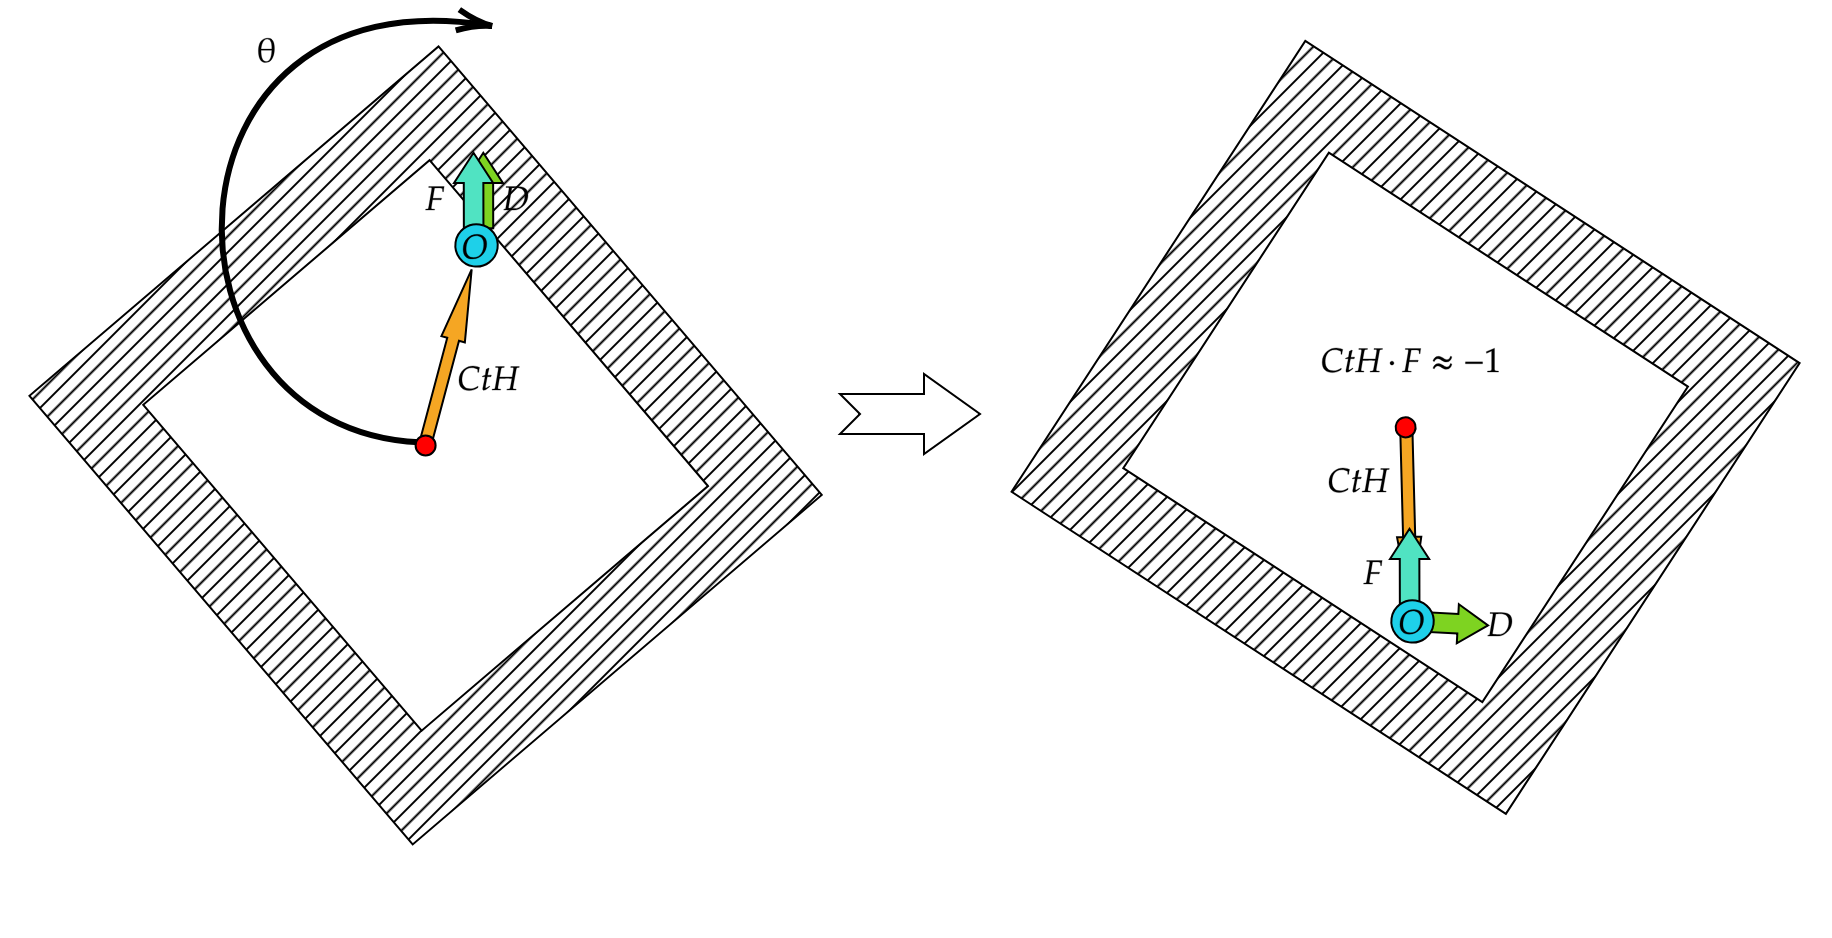
\includegraphics[width=\textwidth]{figures/graphs/AC2F.png}
  \caption[Align Centre to Future Algorithm Example]{AC2F aims to choose the rotation gains that brings the physical centre to head ($CtH$) vector in alignment with the future virtual walking direction ($F$) of the user. The user's current facing direction ($D$) is not used other than setting the value of $F$ as the algorithm starts. The origin of this reorientation is at the position of the user ($O$)}
  \label{fig:ac2f}
\end{figure}

* The way that the real world ''rotates'' depends on what gain is applied to the user and what direction they are moving their head in. 
   * The optimal gain is directly calculated at runtime, but it is technically possible to just choose one depending on the direction you want to rotate relative to what direction the user's head moves in


* Figure~\ref{fig:ac2f}
* Code specific implementation details. 
* Based on what Peck et al. + Chen and Fuchs have mentioned in their work. 
   * No source code was available from their work, as such AC2F is somewhat based on Azmandian et al.'s S2C implementation, but the final result is fairly different from S2C.


\section{The ''Pause - Turn - Centre'' Resetter}\label{sec:pauseturncentre}
* Inspired by freeze turn (CITE creator)
* Also takes inspiration from what Sra et al. have mentioned
   * Limiting visibility makes changes less noticable
   * In this case, the virtual world is "paused", resulting in a rotation gain of 0, but this is masked by mostly fading it to black and overlaying a representation of the physical space on top. 
* Clipping problem
   * How is it solved?
       * Double camera solution, forcing different depth levels so one camera always will draw over what the other does
   * What are the pros/cons of this solution?
      * Easy to implement
      * Costs some performance
         * Especially if post processing is used. 4 cameras in total, each needing to do post processing is costly.
            * There is some granularity here though. For example it is possible to control what PP is applied to the virtual/physical spaces. Less can be applied to the physical space as it is not seen as often.

\subsection{Pausing the Game Using ''Pause - Turn - Centre''}
* All dynamic objects in the game use a specific pausable class as their parent. 
   * This includes any projectiles, distractors and other animated components.
* The redirectionManager is then able to find a list of all objects that derive from this pausable class when resetting is necessary. It then triggers a callback for each of these so they can take care of pausing their own behaviour. 

\section{Supporting the Y axis in the RDW toolkit}
   * Basically a bugfix to the way the toolkit worked
   * an issue with the body follower not working with the Y axis. 
   * This change was put into the toolkit itself as it was more of a bug rather than a major change.

\section{Game Design Overview of Ensemble Retriever} 
In Ensemble Retriever, the player takes the role of a conductor whose goal is to retrieve the ''Mountain King'', which is an instrument that has disappeared from their ensemble. In order to find the ''Mountain King'', the player has to walk around in a large virtual environment and ask the local residents for clues before they can enter the ''Hall of The Mountain King''. Throughout the player's exploration of the virtual world, they are attacked by various distractor enemies which have to be defeated to gain experience points and progress the game. These battles consist of having the player use their contrabass shield to absorb enemy projectiles. Once enough projectiles have been absorbed, the player is able to counterattack with their magical conductor baton. The game culminates with a battle against the ''Mountain King'' that tests the player's skill and abilities which they have trained throughout their battles with distractor enemies.  

The following sections provides a more detailed context on the game itself and how distractors have been fully integrated into the experience.

\subsection{Virtual Environment}
* \todo{More Pictures! This one might change right before ex 1 if it takes too long to walk so no need write this until after that}
* Can show roughly how many metres the user has to walk to reach the portal etc. Top down views of the world relative to physical space and so on. 

\subsection{Game Flow}
\todo{Can probably add some pictures}
This section provides an outline of the flow of Ensemble Retriever and how the game progresses throughout a play session. 

Ensemble Retriever starts off with a tutorial that teaches the player the basics of the game. It provides information on the context/story, the player's goal, how to deal with reorientation resets, how to fight enemies and what to do if they are lost. In experiment 1, the tutorial also provides information on what the player should do if they notice they are being redirected. 

After the tutorial is finished, the game transitions to a walking phase where the player tries to reach the ''Hall of The Mountain King'' while being encouraged to visit three green fireflies that provide hints which will be relevant for a later part of the game. As the player walks around in this phase, distractor enemies will appear once they hit the maximum safe distance away from the centre. These enemies need to be defeated to progress and award experience points that the player can use to either upgrade the size of their contrabass shield or the damage that their conducting baton does. It should be noted that the fireflies fade away during battles to prevent their salience from potentially affecting the attention of the player since this could result in lower concentration~\cite{sitzmann2018saliency}. The walking phase of Ensemble Retriever is finished once the player enters the portal to the ''Hall of The Mountain King''. 

Once the player enters the ''Hall of The Mountain King'', any redirection gains are disabled. This is to allow the player to spend the last few minutes of the game getting used to normal head rotations before taking off the HMD. Inside the hall, the player has to answer a multiple choice quiz which asks questions based on the previous hints that could have been acquired from fireflies in the walking phase. The quiz itself cannot be failed, but the final score that the player is given ties with how many correct answers they give. The quiz itself has three questions in total.

Once the quiz is finished, the player will have to fight against the ''Mountain King''. This is a longer battle where the ''Mountain King'' will use combinations of all previous attacks that distractor enemies have been using to challenge the player. Once the ''Mountain King'' has been defeated, the game is finished and the player will be shown their scores which consists of four components:
\begin{enumerate}
    \item Time Score (How long it took to finish the game. Shorter times means higher scores)
    \item Damage Score (How much damage the player has taken in total. Less damage means higher scores)
    \item Quiz Score (How many correct quiz answers the player has gotten)
    \item Total Score
\end{enumerate}

\section{Fully Integrating Distractors with Game Mechanics}
\begin{figure}[tbph]
    \centering
    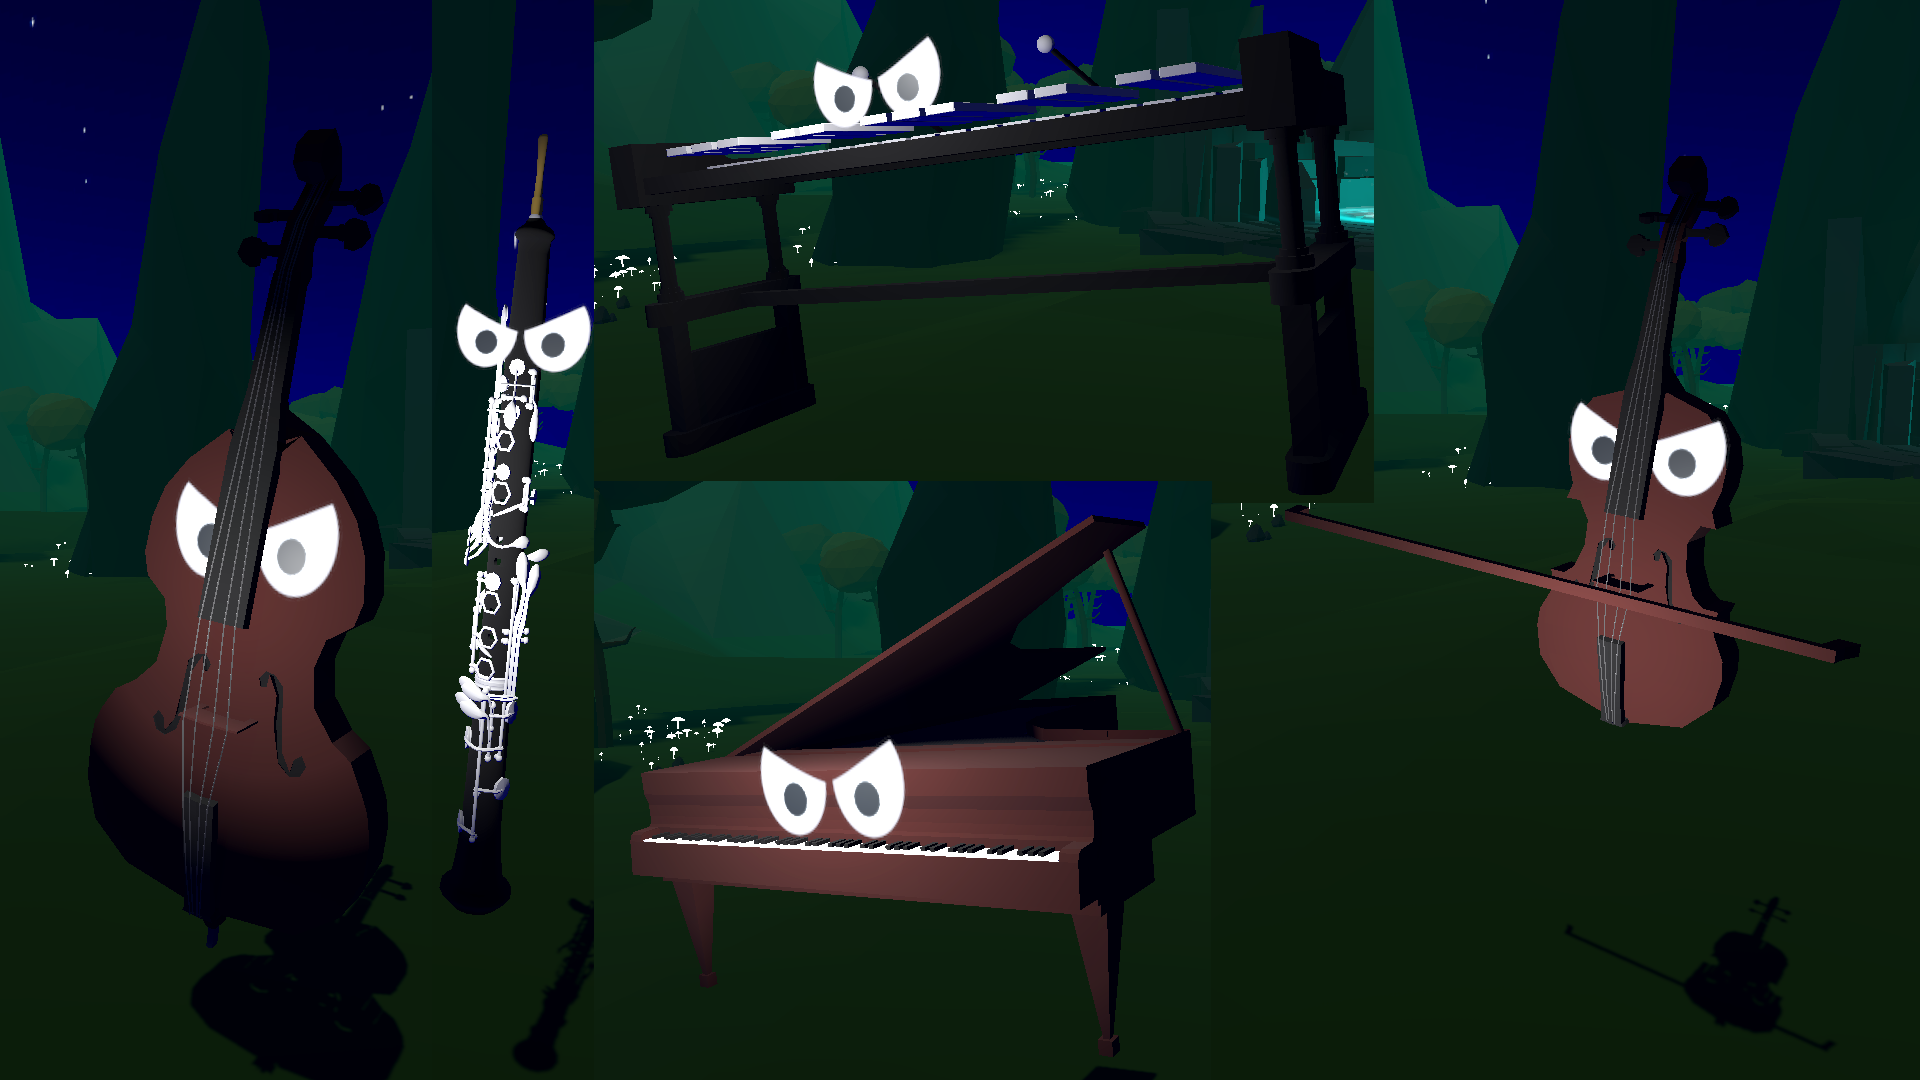
\includegraphics[width=1\textwidth]{figures/screenshots/Distractors.png}
    \caption[The Distractors of Ensemble Retriever]{These are the five distractor enemies that are employed in the Ensemble Retriever game.}
    \label{fig:allDistractors}
\end{figure}

The development resource budget of Ensemble Retriever was fairly small(\textasciitilde1.25 months). As such, in order to have a reasonable scope and allowing for as much code/asset reuse as possible, the main mechanic that was decided to fully integrate with distractors was the enemy encounters in the game. Since the AC2F algorithm relies on rotation gains, the goal of using distractors in this case was to make the player move their head around as much as possible. Ensemble Retriever currently consists of five enemy distractors which can be seen in Figure~\ref{fig:allDistractors}. If we look back to the taxonomy of distractors which was presented in Section~\ref{sec:distractorTaxonomy}, these can be considered as explicit, concrete distractors that are fully integrated into the experience. In this case, the distractors are considered explicit as the player is told they have to fight them. 

From a game design point of view, their use can be seen as ''random'' enemy encounters which is a common mechanic in role playing games. Instead of actually being random though, these enemy encounters trigger once the player has reached the maximum safe distance away from the centre of their physical tracking space. 

Once an enemy encounter starts, one of the five possible distractors are randomly chosen from a list. The chosen distractor is then removed from this list so it cannot be chosen again for some time. Once all distractor enemies have been chosen from the list, it is then repopulated with all five again. In the worst case scenario, this means that the same distractor might show up as the next enemy right after the list has been repopulated. The rationale for this approach is to avoid situations where the same distractor can show up too many times in a short space of time, potentially annoying the player due to limited variety as mentioned by Sra et al.~\cite{sra2018vmotion}. 

Each of the five distractor enemies rely on projectile attacks that have three potential movement speeds as well as a unique property per type of distractor. Before attacking, the distractor will make use of two telegraphs: one for the type of projectile it will attack with and one for how fast it will be. These telegraphs make use of both animation and audio cues, allowing the player to learn and identify the different types of attacks that are used so they can prepare accordingly. 

A standard enemy encounter consists of two phases: a tutorial phase and a proper battle phase. During the tutorial phase, the distractor will use its different attacks in order to teach the player its capabilities. In this phase, the distractor will not move away from its initial position. Once the player manages to counterattack the distractor, the real battle begins. During the battle phase, the distractor will randomly choose an angle between -360 and 360 degrees from the player after each attack, and rotate around them. The attack order will at this point also either be random or predetermined depending on the type of distractor. This forces a fair amount of head rotation from the player as they need to keep track of where the distractor moves and where their projectile attacks are. This also makes good use of the full 360 degree space that virtual reality allows while providing many opportunities for applying rotation gains.    

The following sections will describe and detail each distractor that exists in Ensemble Retriever. It should be noted that the screenshots of these were taken from the debug mode of the game, hence why the conductor baton and shield are in fixed screen positions.

\subsection{The Contrabass}
\begin{figure}[tbph]
    \centering
    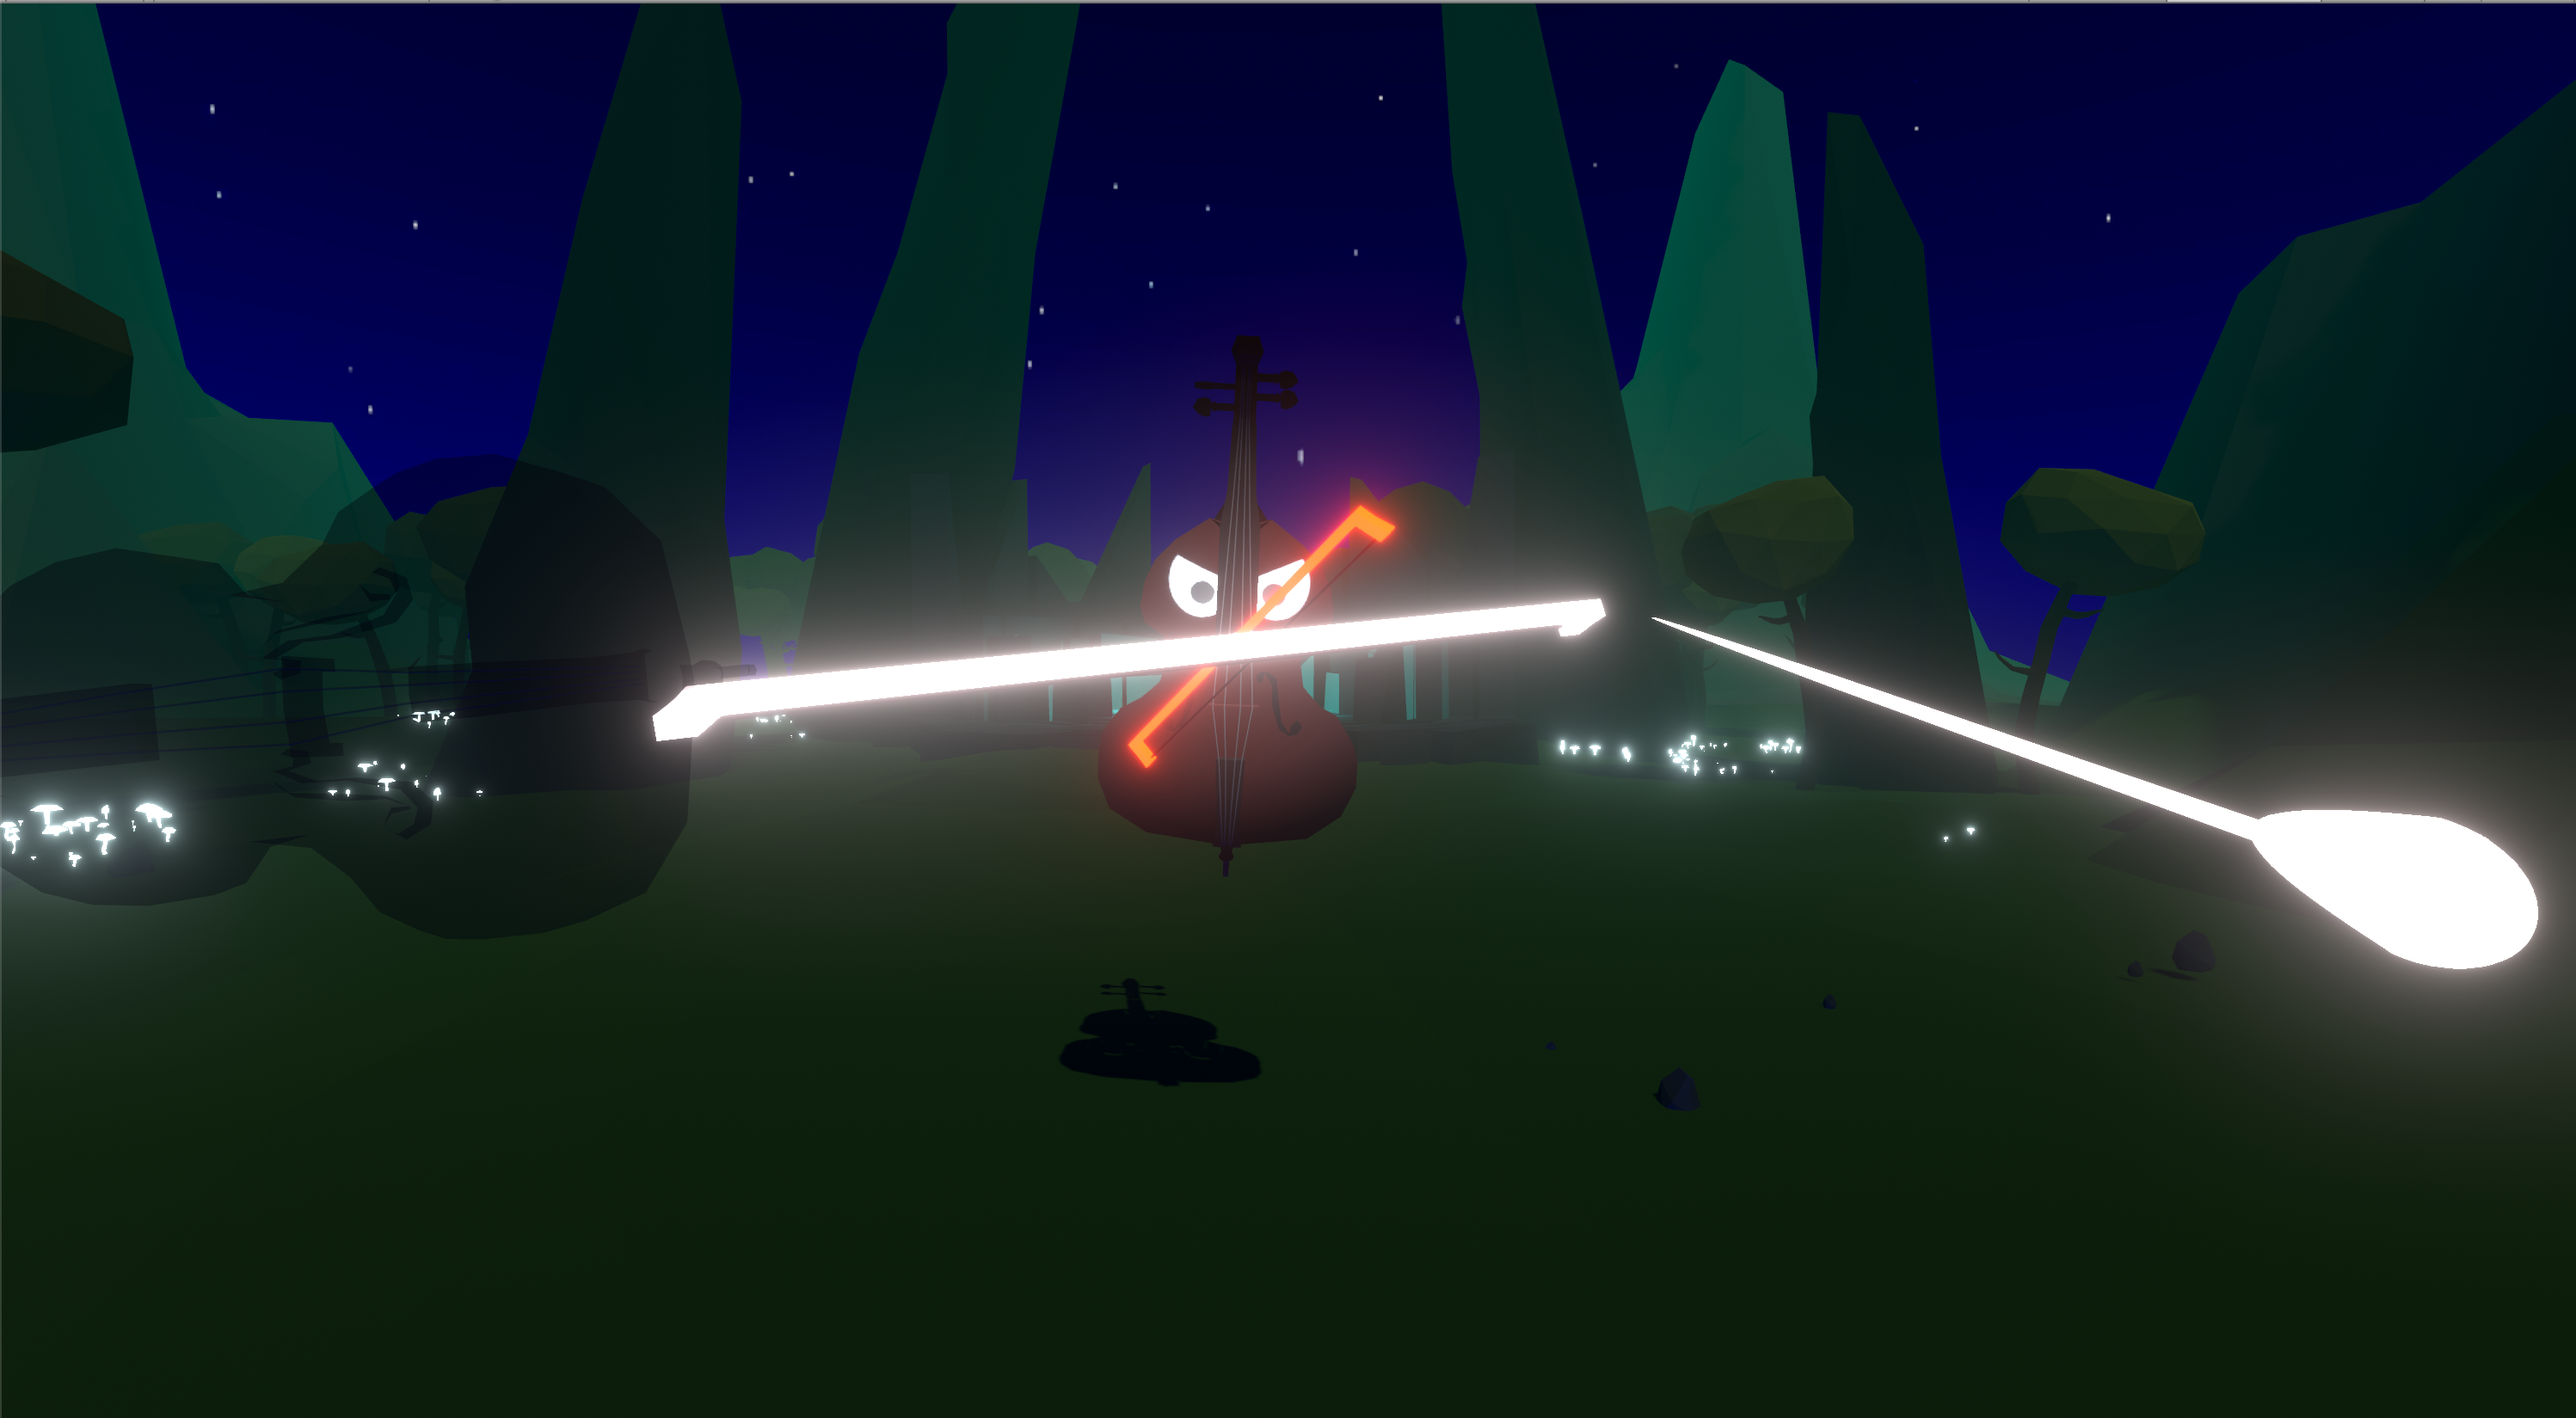
\includegraphics[width=0.75\textwidth]{figures/screenshots/contrabass.png}
    \caption[The Contrabass Distractor]{This screenshot shows off the contrabass distractor and its projectile attacks which travel directly towards the player.}
    \label{fig:contrabassDistractor}
\end{figure}
The first among the five distractor enemies is also the simplest one: ''The Contrabass'' as seen in Figure~\ref{fig:contrabassDistractor}. It attacks the player with projectiles that simply move towards them in a straight line. As a means to make the player move their head around more, the contrabass will mix slow and fast projectiles. A fast projectile will in this case move fast enough that it hits the player before a previously thrown slow projectile. This way, the player has to keep track of where the contrabass itself is when it uses fast projectiles while trying to remember where the slower moving ones are so they can absorb these as they come close. 
 
\subsection{The Oboe}
\begin{figure}[tbph]
    \centering
    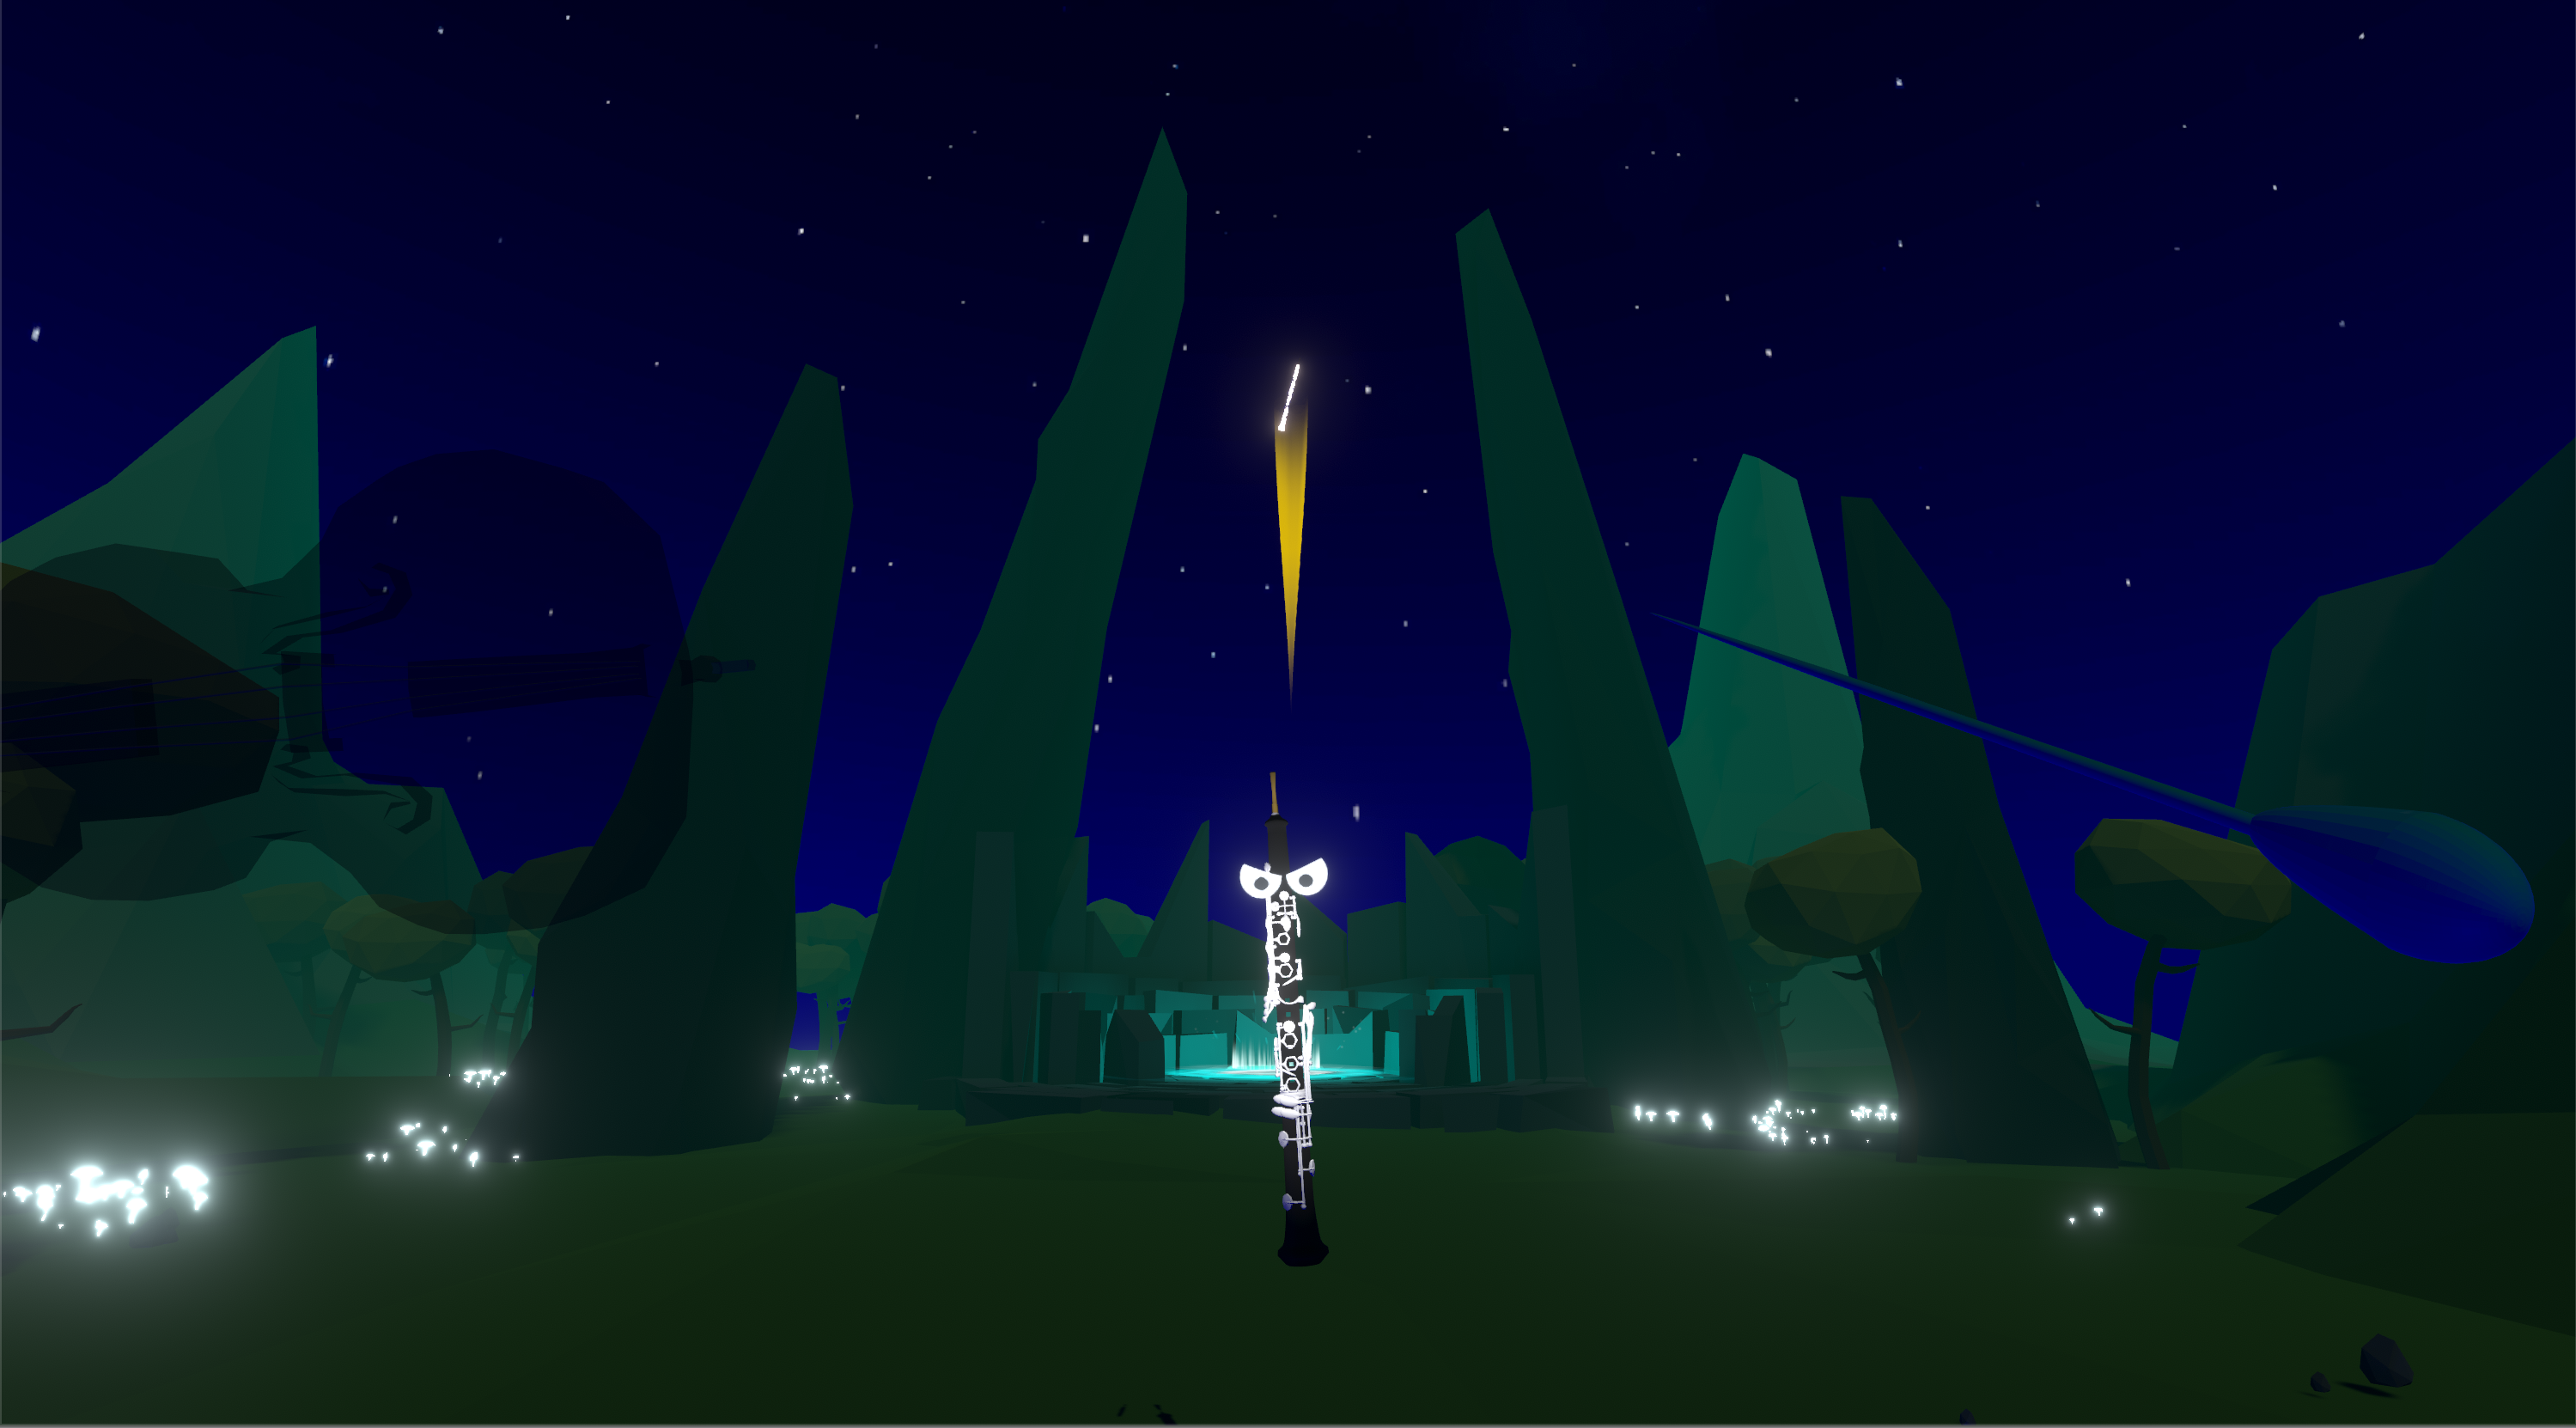
\includegraphics[width=0.75\textwidth]{figures/screenshots/oboe.png}
    \caption[The Oboe Distractor]{This screenshot shows the oboe distractor and its projectile attack which will travel on a vertical arc above the head of the player.}
    \label{fig:oboeDistractor}
\end{figure}

\begin{figure}[htbp]
  \centering
  \includesvg[width=0.5\textwidth]{figures/svgs/oboeProjectile.svg}
  \caption[Sideways 2D Example of Oboe Projectile Path]{An illustrated, sideways 2D example of how the oboe projectile travels. The blue circle and quad represents the player while the red circle represents the distractor that is about to attack.}
  \label{fig:oboeProjectile}
\end{figure}
The next distractor is ''The Oboe'' which can be seen in Figure~\ref{fig:oboeDistractor}. It attacks the player with projectiles that move in a vertical, 180 degree arc above the player's head before travelling straight towards their head. A rough two dimensional figure illustrating this can be found in Figure~\ref{fig:oboeProjectile}. The Oboe attempts to facilitate head rotation by trying to hit the player from behind with projectiles. A clever player might end up holding the shield behind their head to absorb these, lessening the impact of the approach though. Despite this, it is still necessary to keep track of the projectiles as the Oboe moves and rotates around the player. 

\subsection{The Harpsichord}
\begin{figure}[tbph]
    \centering
    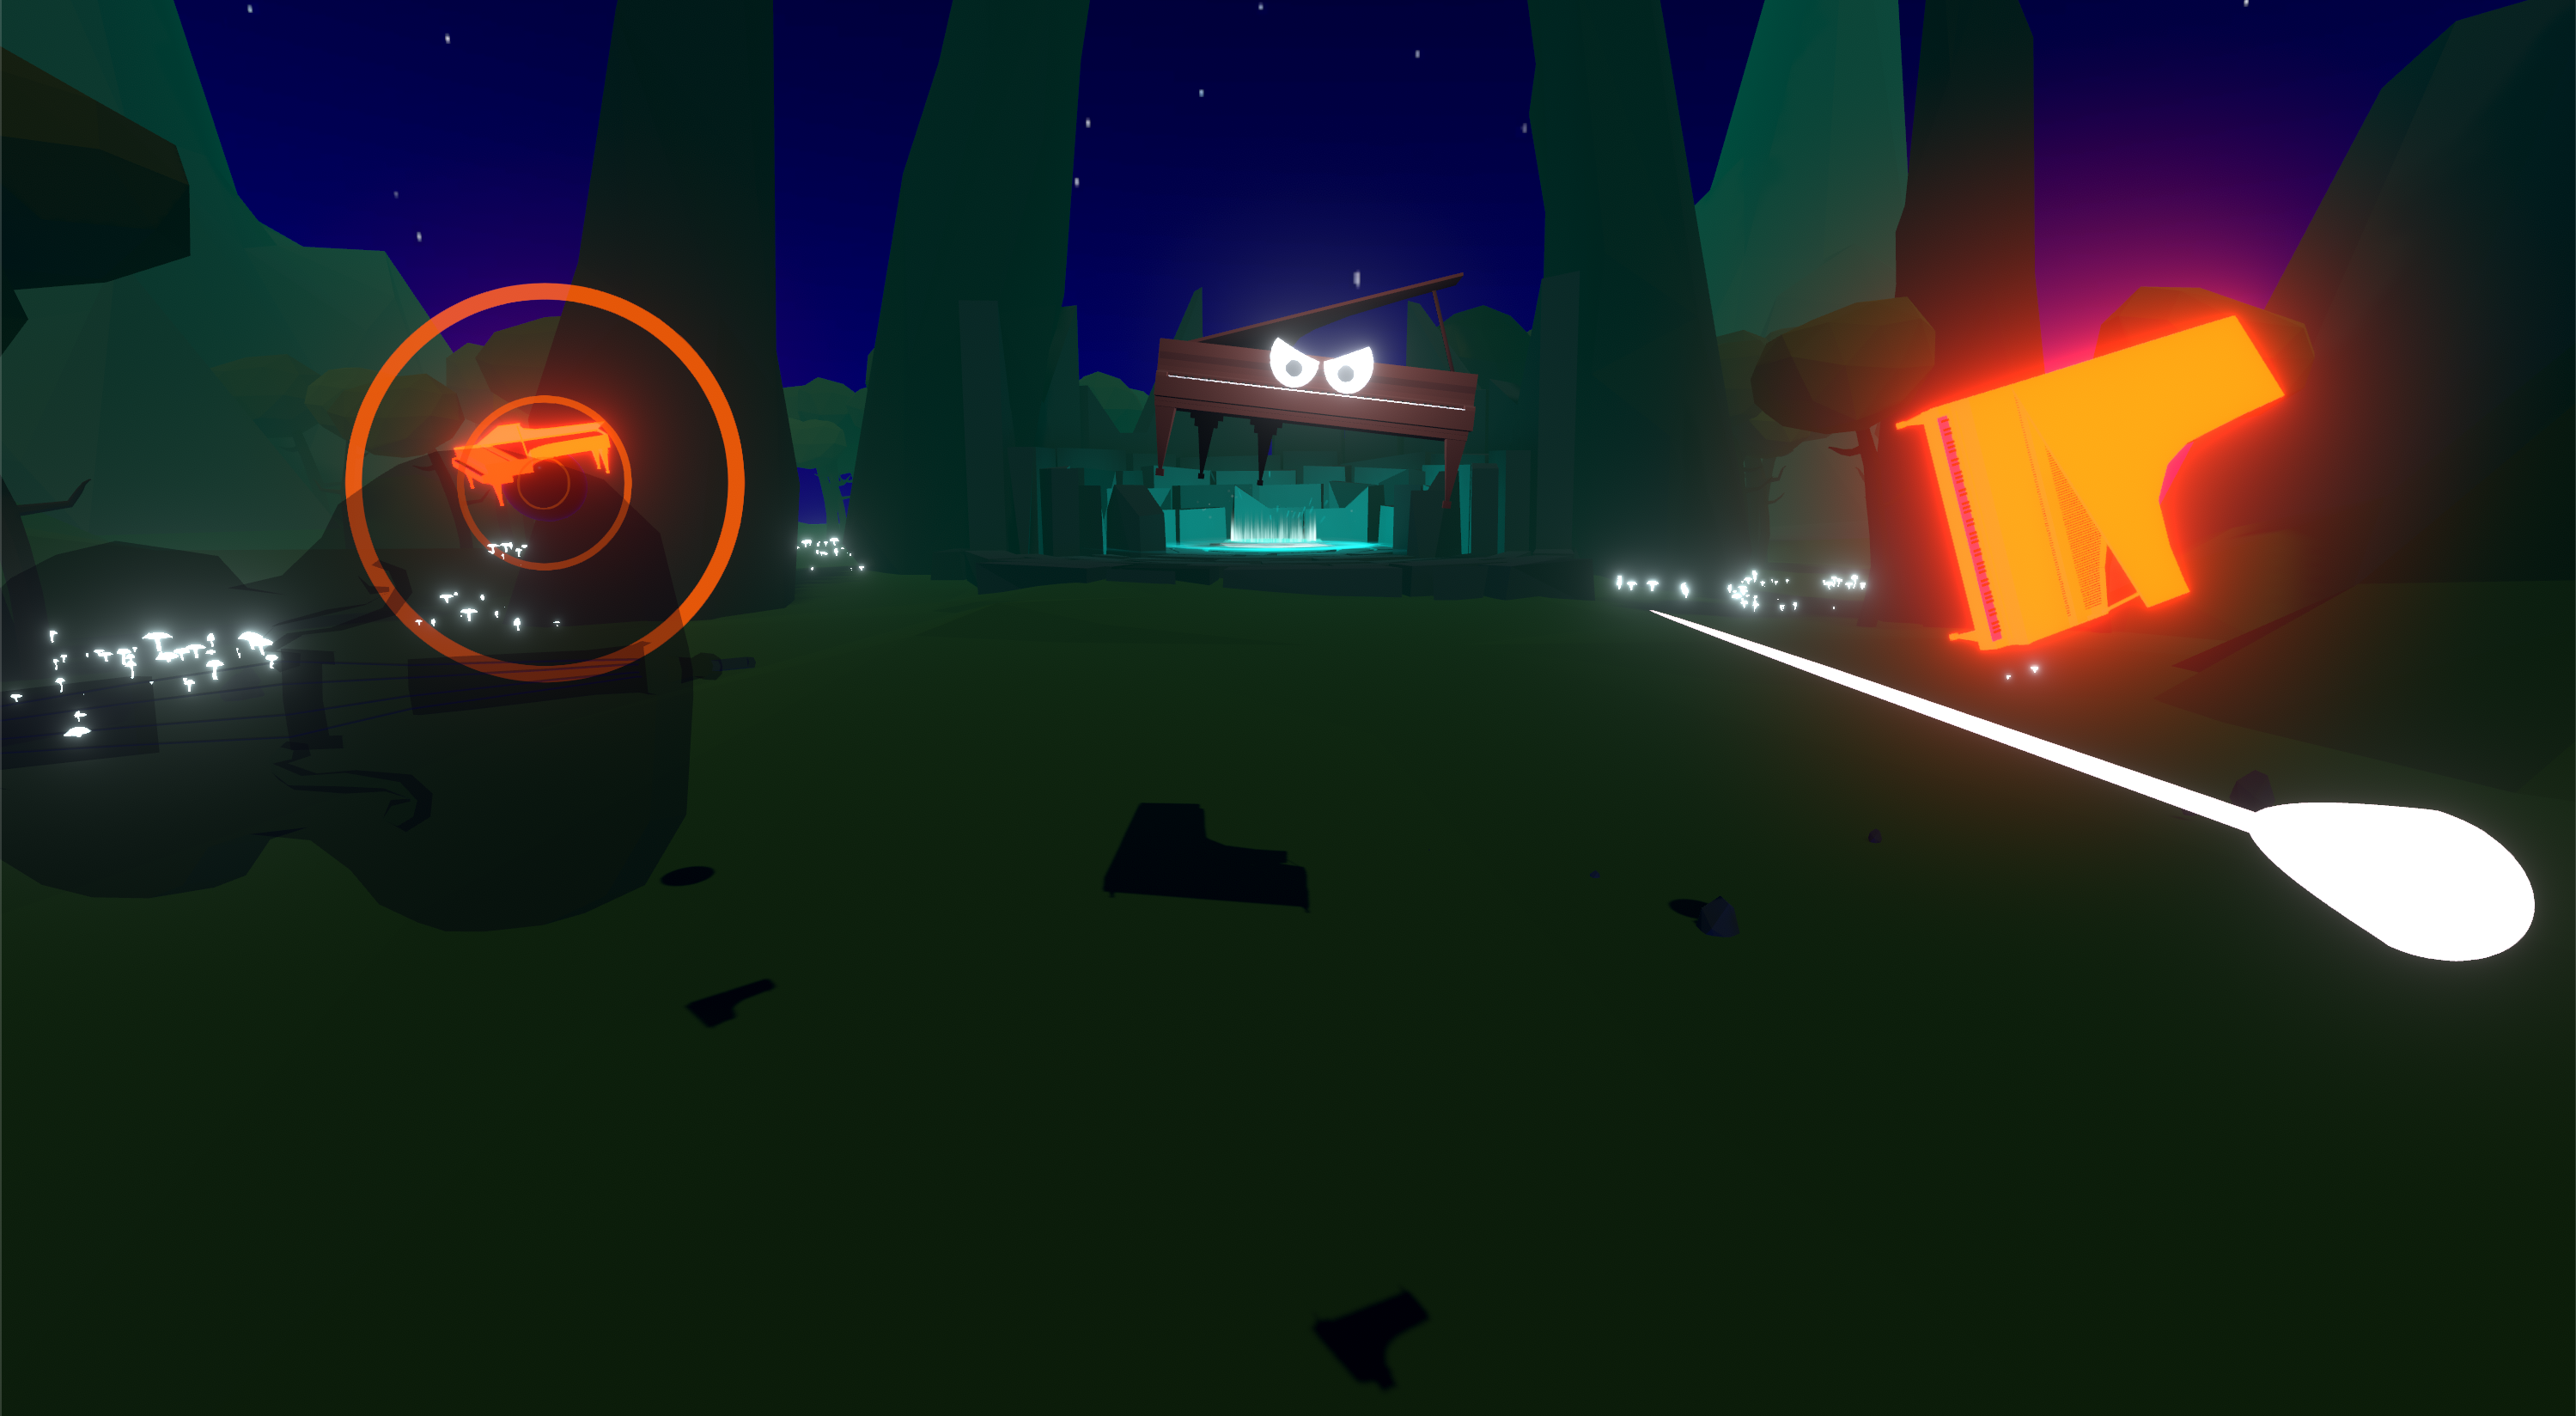
\includegraphics[width=0.75\textwidth]{figures/screenshots/harpsichord.png}
    \caption[The Harpsichord Distractor]{This screenshot shows the harpsichord distractor. It attacks with multiple rapid projectiles from two locations which are further away from its body.}
    \label{fig:harpsichordDistractor}
\end{figure}
''The Harpsichord'' which can be seen in Figure~\ref{fig:harpsichordDistractor} is the third distractor in Ensemble Retriever. It attacks the player with rapid projectiles that spawn from two wormholes that are further away from its body. This means that the player needs to move their shield from left to right to quickly block incoming projectiles. It allows for some extra head rotation as the player might need to slightly shift their head to clearly see each projectile. 

\subsection{The Violin}
\begin{figure}[tbph]
    \centering
    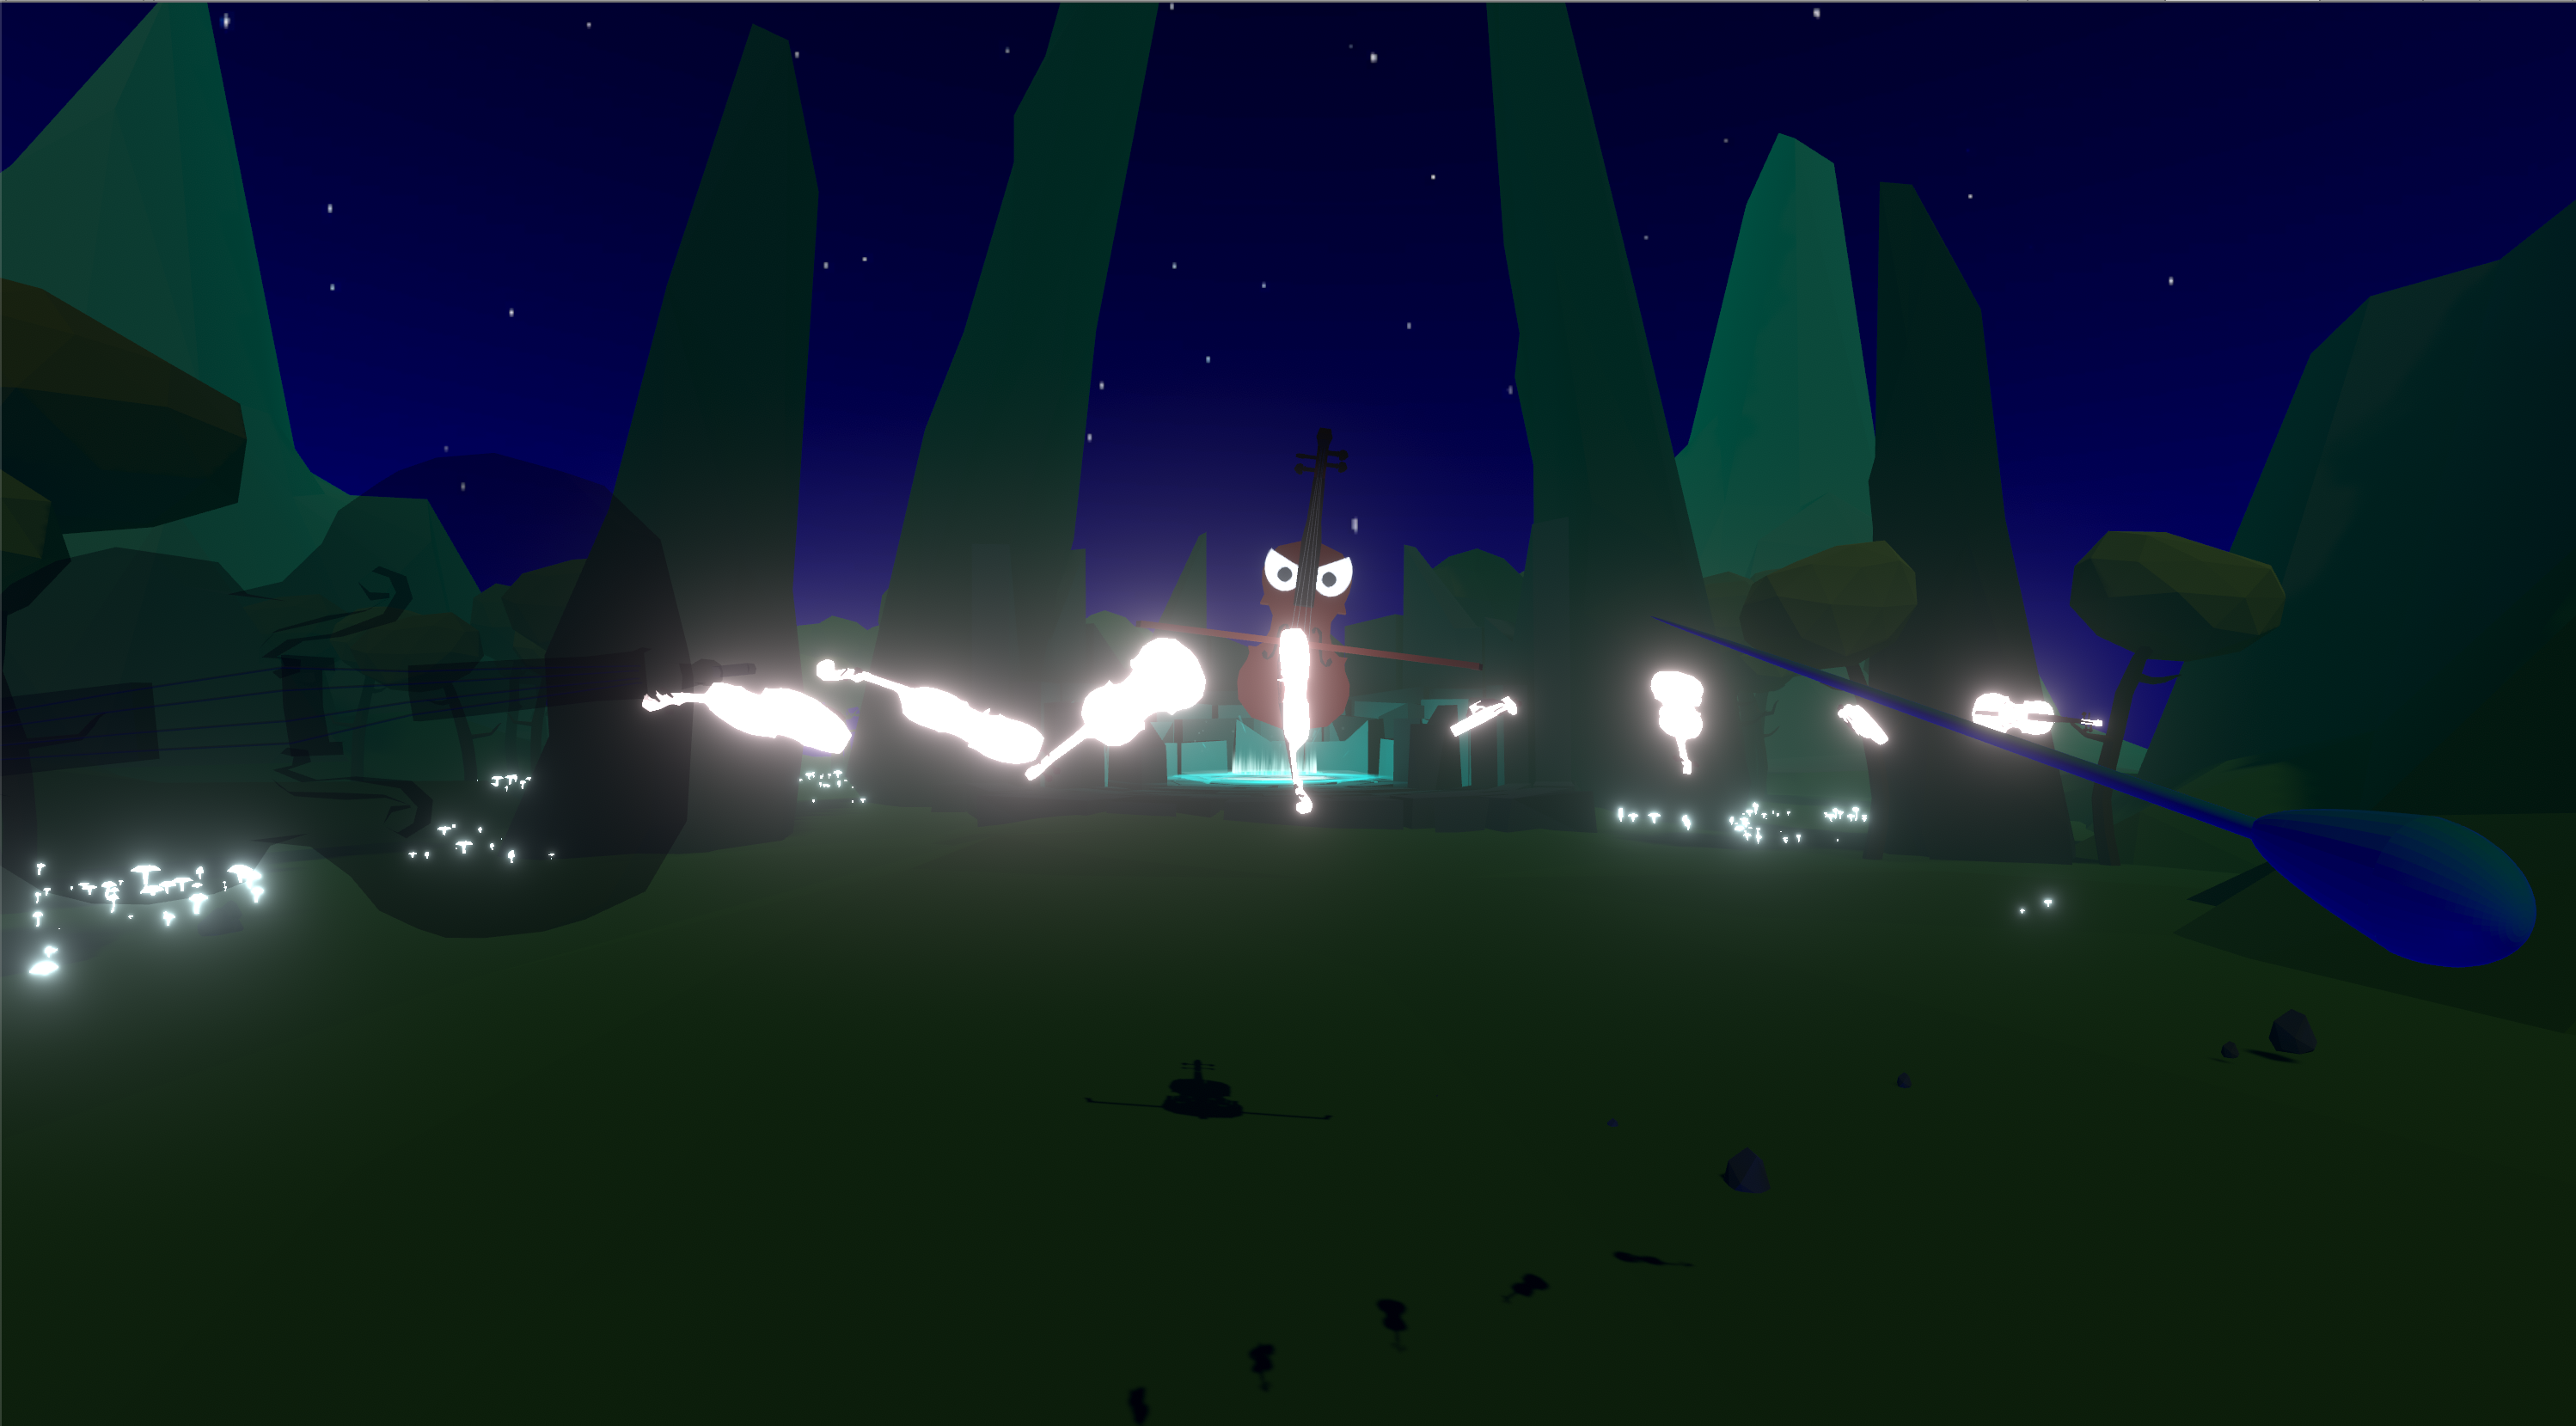
\includegraphics[width=0.75\textwidth]{figures/screenshots/violin.png}
    \caption[The Violin Distractor]{This screenshot shows the violin distractor. It attacks with several projectiles at a time in a line formation.}
    \label{fig:violinDistractor}
\end{figure}
The fourth distractor in Ensemble Retriever is ''The Violin'' which can be seen in Figure~\ref{fig:violinDistractor}. It is similar to the Harpsichord in the regard that it rapidly fires projectiles. Instead of firing projectiles from two locations though, it instead fires a line of projectiles that the player needs to block with their shield. This allows for some additional head rotation as the player needs to trace the line of projectiles that moves towards them. The line itself is long enough that some shifting of head orientation is beneficial to see everything as it gets close. 

\subsection{The Glockenspiel}
\begin{figure}[tbph]
    \centering
    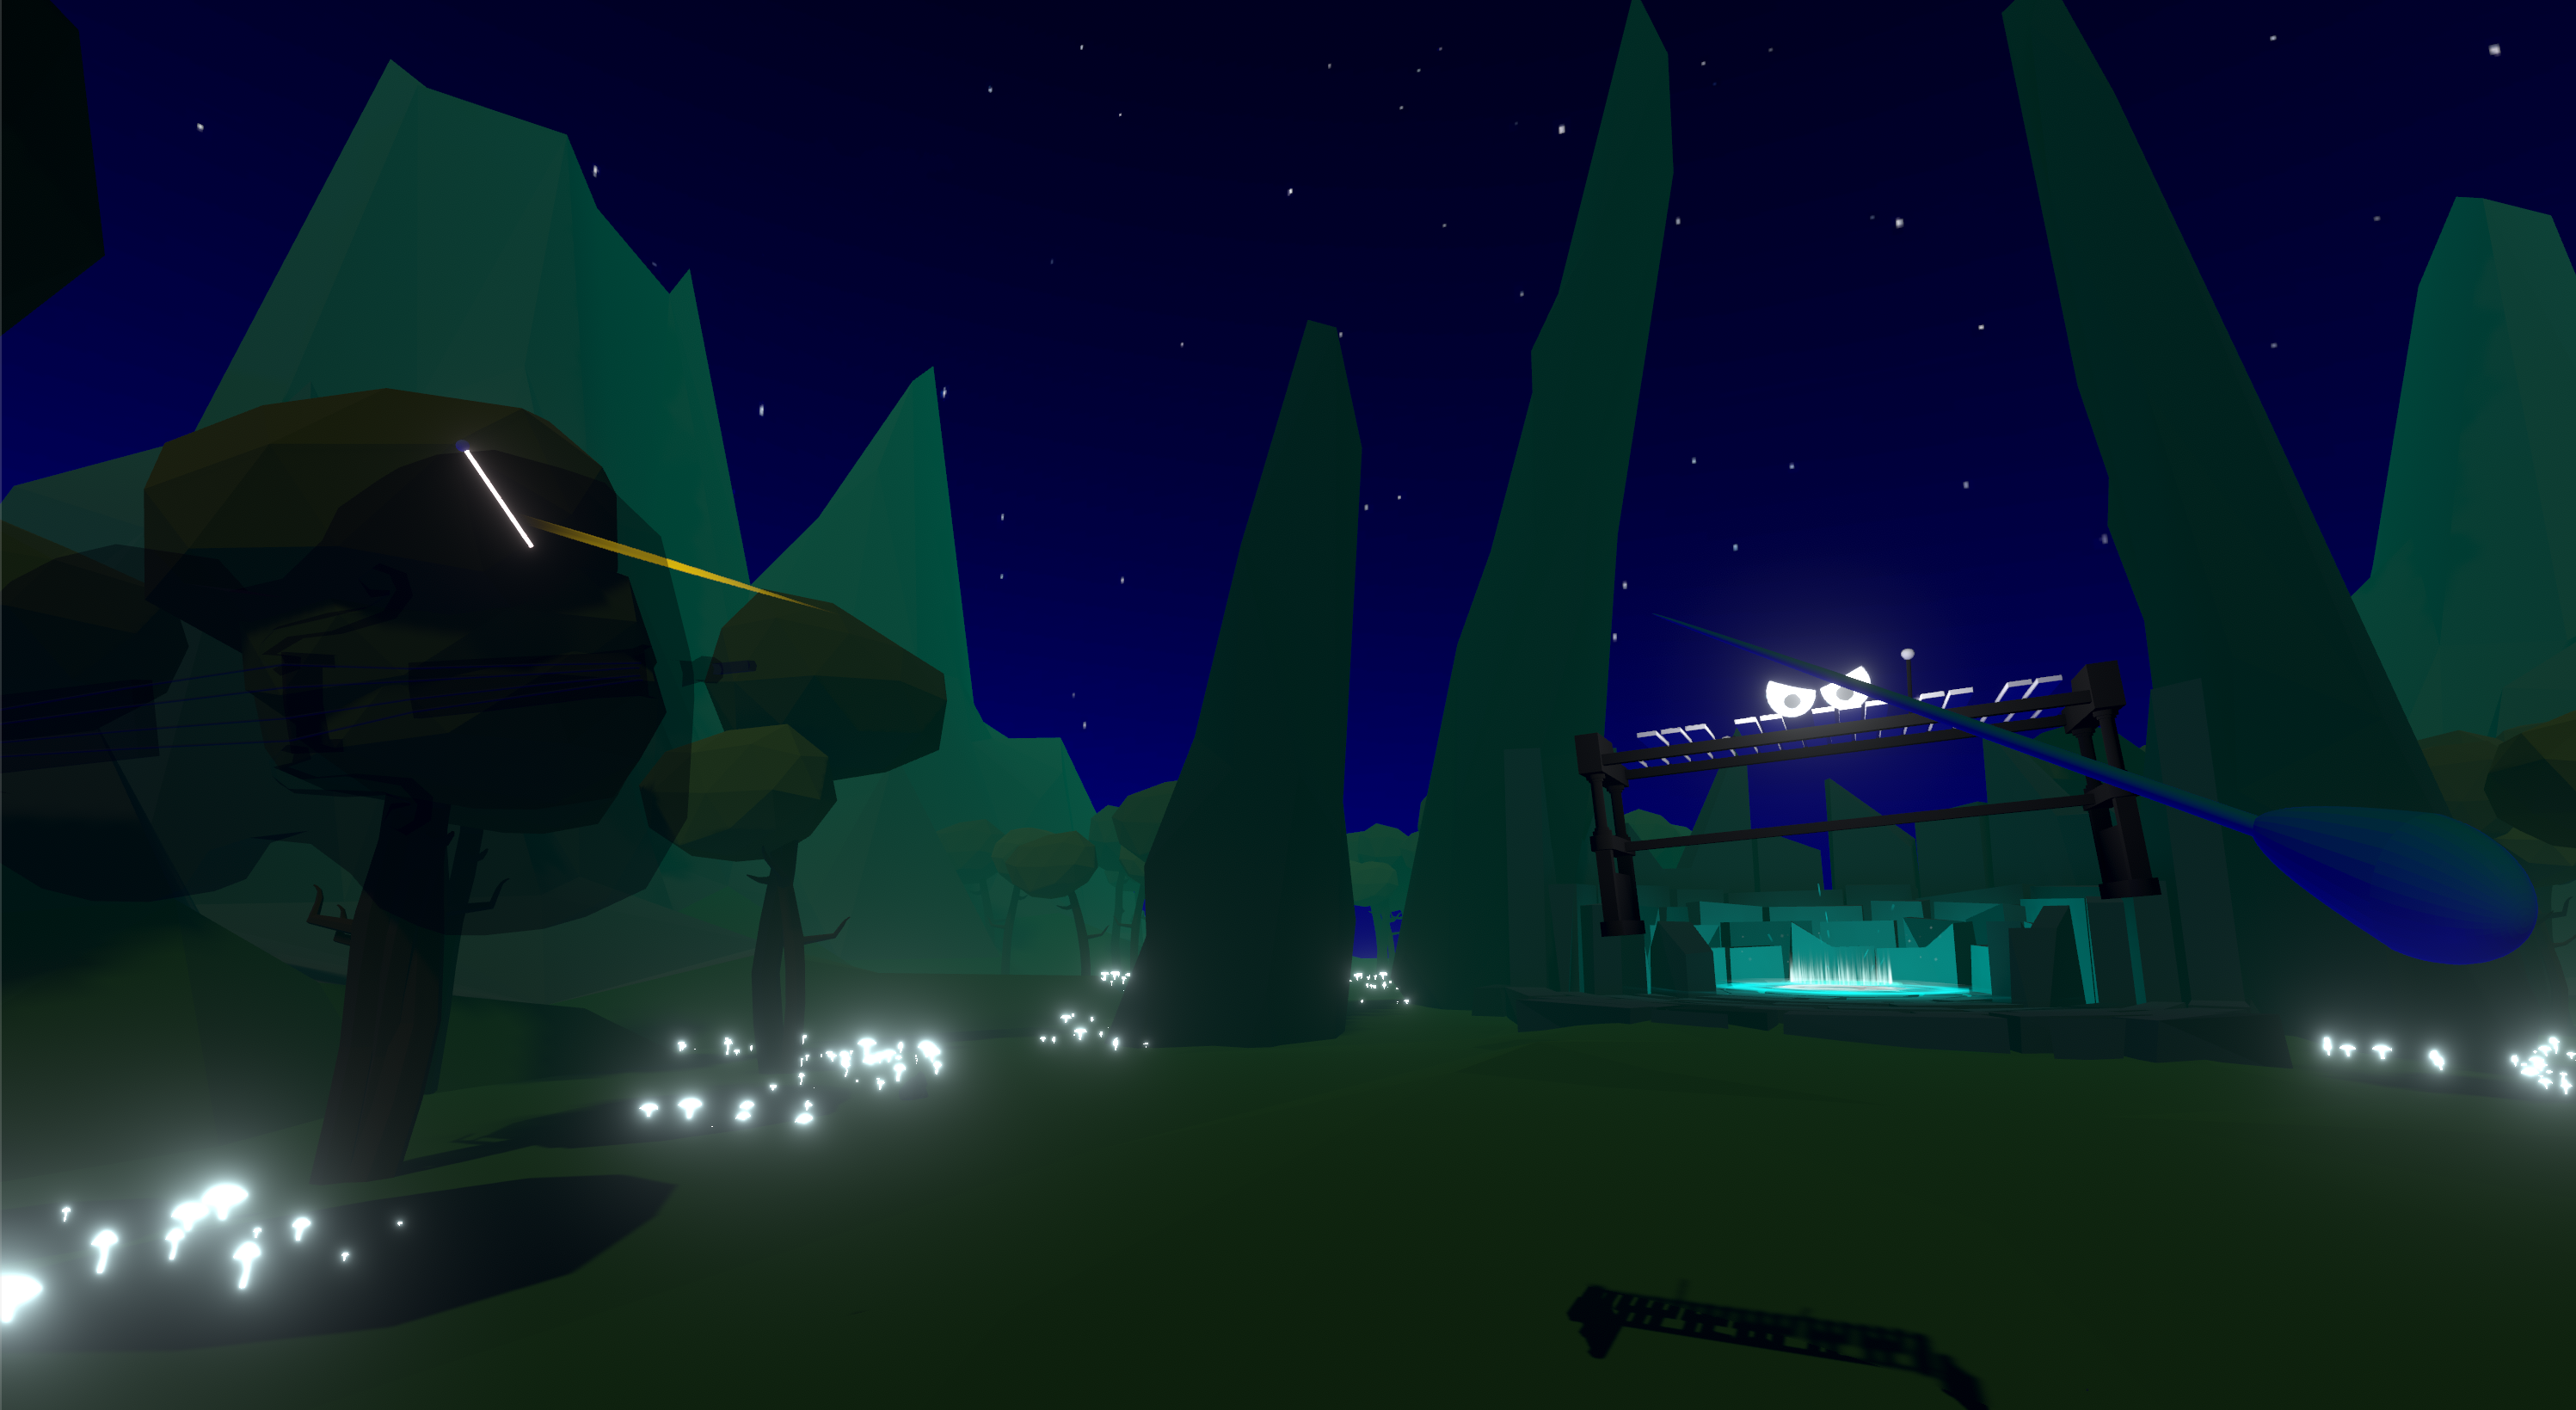
\includegraphics[width=0.75\textwidth]{figures/screenshots/glockenspiel.png}
    \caption[The Glockenspiel Distractor]{This screenshot shows the glockenspiel distractor and its curved projectile attack. The projectile itself travels on a \textasciitilde90 degree arc towards the player's left side.}
    \label{fig:glockenspielDistractor}
\end{figure}
Finally, we have ''The Glockenspiel'' which is seen in Figure~\ref{fig:glockenspielDistractor}. This distractor attacks the player by throwing projectiles that travel on a curve towards the player. The curve itself will intersect with the player at a roughly 90 degree angle to their left from where the projectile was fired. This facilitates more head rotation as the player needs to track the path that the projectile flies through before blocking. 

\section{Employing Context Sensitive Resets: Teleporters}
* Other researchers have looked into context sensitive reorientation outside of distractors haven't they? Double check!
* Can draw some comparisons to Suma et al.'s change blindness redirection.
   * Instead, in this case: it is possible to exploit the user's lack of knowledge with a future location to allow for reorientation. 
* As the player enters the portal, their facing direction after being teleported is changed in a manner so that the path they have to walk to continue is back towards the room centre.
* This is an example of an alternative context sensitive means of reorienting the user
* While it cannot be expected that a game is sprinkled with teleporters everywhere, this can be seen as a useful tool to use once in a while if you want to move the player to different locations and environments
* There are of course many other ways to also implement context sensitive resets. 
   * An elevator could for example be used for it
   * Anything in general that limits visibility or vision of the target destination can technically be used to create context sensitive reorientation in the same vein as this.
      * Very similar to what Sra et al. have already discussed in terms of limiting visibility for redirection and reorientation

\section{Disabling Redirected Walking Towards The End of an Experience}
* Throughout the final stretch of the game, redirection gains are disabled as a means of helping participants get used to normal head rotations before taking off the HMD.
* How effective this approach is, would of course need to be further tested in a separate study, but it should at least help somewhat normalise the head rotations for the user before finishing.
* Might not be easy to integrate with every solution, but in the case of Ensemble Retriever since the final portion is just to fight the Mountain King, there wont be much more movement involved so it is fine. 
\chapter{Experiment 1: Noticability of Distractors}\label{chap:ex1}

\section{Method}
* The average gains end up being for the specific population we test with

* Disclaimer before start of the game
   * Try to avoid moving around too much in combat as you wont be able to see the chaperone

\subsection{Performance Data Collection}
* Lots of things recorded every frame. List it all

\subsection{Sample}
\section{Results}\label{sec:ex1results}
This part of the chapter provides the results of the experiment related to the established $H_0$ hypothesis as well as insights from demographical data. Data visualisation for these results is provided by SPSS due to the large data file sizes. A significance level of 0.05 was used for all statistical tests. For the sake of disclosure for any graphs that directly mention participant ID's, the author's ID is 16. It should also be noted that the participant with ID = 10 is excluded from the sample due to prior mentioned reasons. In terms of presentation, the majority of the graphs will be comparing the S2C and AC2F algorithms as they respectively represent the walking and battle states in Ensemble Retriever.

\subsection{Rotation Detections}
As the main focus of Experiment 1 was on detection thresholds, these first few sections are dedicated to presenting the graphs over detection events for participants as they played Ensemble Retriever. Detected rotation gains are initially presented with curvature radius detections following this.

\subsubsection{Raw Rotation Detections Sample}
\begin{figure}[tbph]
    \centering
    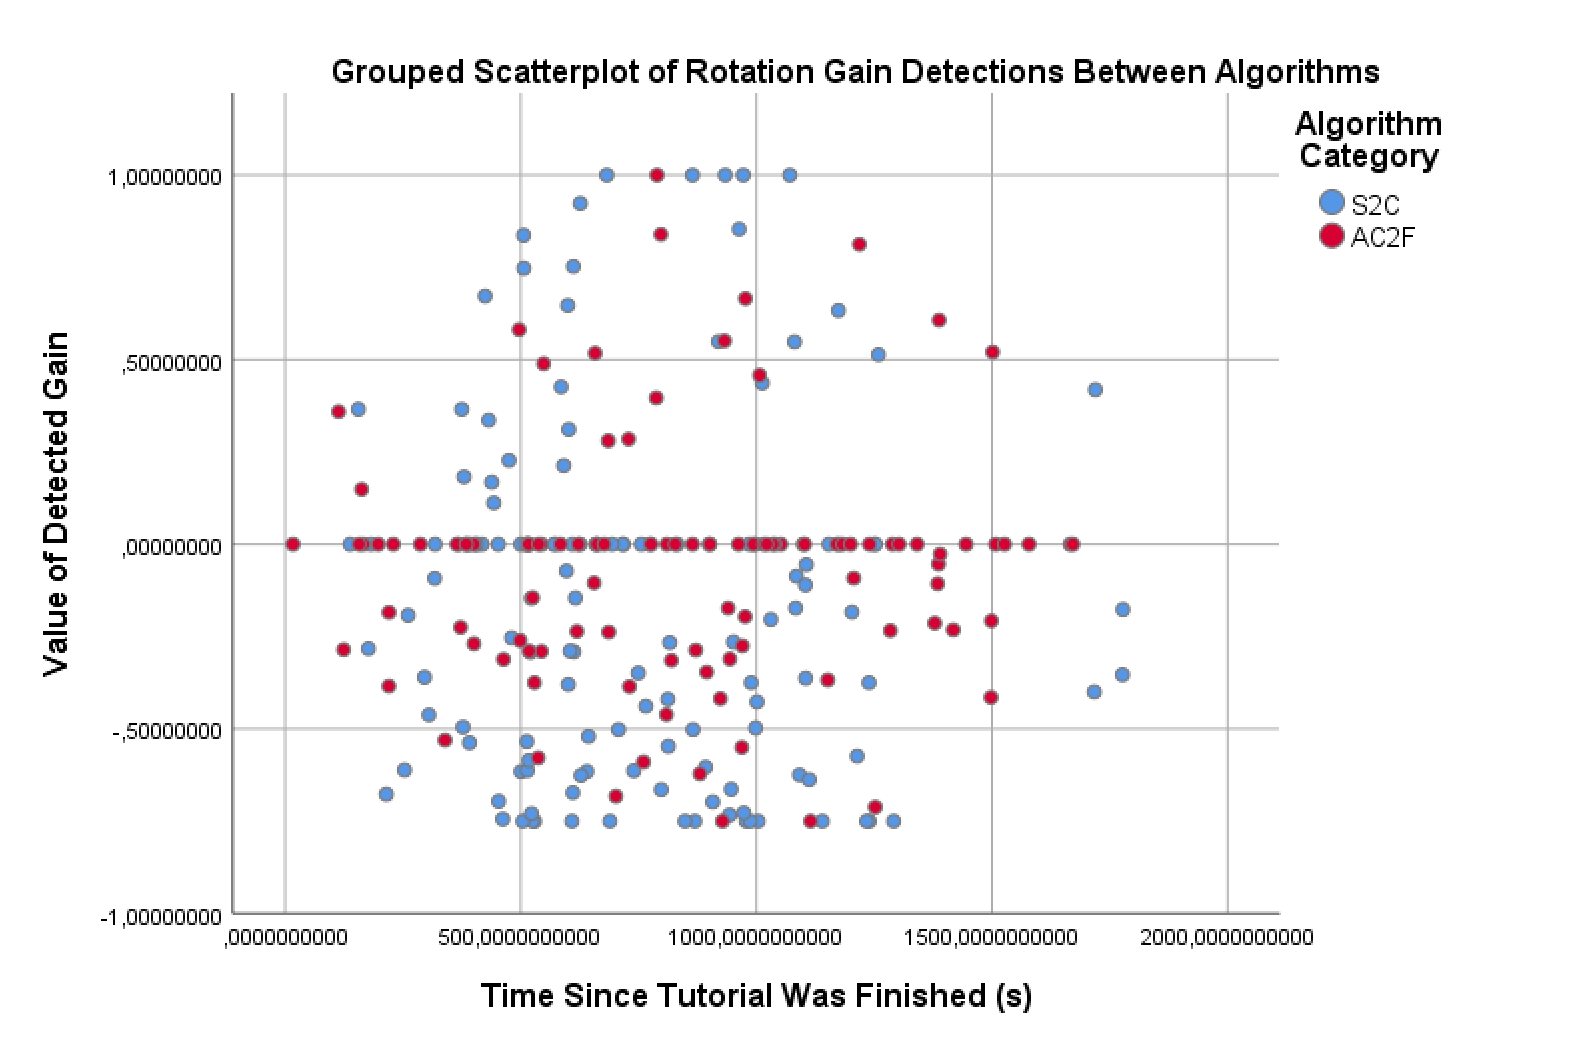
\includegraphics[width=0.75\textwidth]{figures/graphs/RawRotationDetections.png}
    \caption[Raw Detection Scatterplot For Rotation Gains]{This scatterplot shows the raw data, including outliers for rotation detections between the two employed algorithms. S2C is used for the walking state while AC2F is used for the fighting state.}
    \label{fig:rawRotationDetectionData}
\end{figure}

Before seeing the post-processed sample of rotation gain detections, it might be interesting to first see how the raw data looks like. This raw data can be seen in Figure~\ref{fig:rawRotationDetectionData}. The various cases where detected gains are at a value of 0 is what the post-processing step aimed to minimise. 

\subsubsection{Finalised Rotation Detections Sample}
\begin{figure}[tbph]
    \centering
    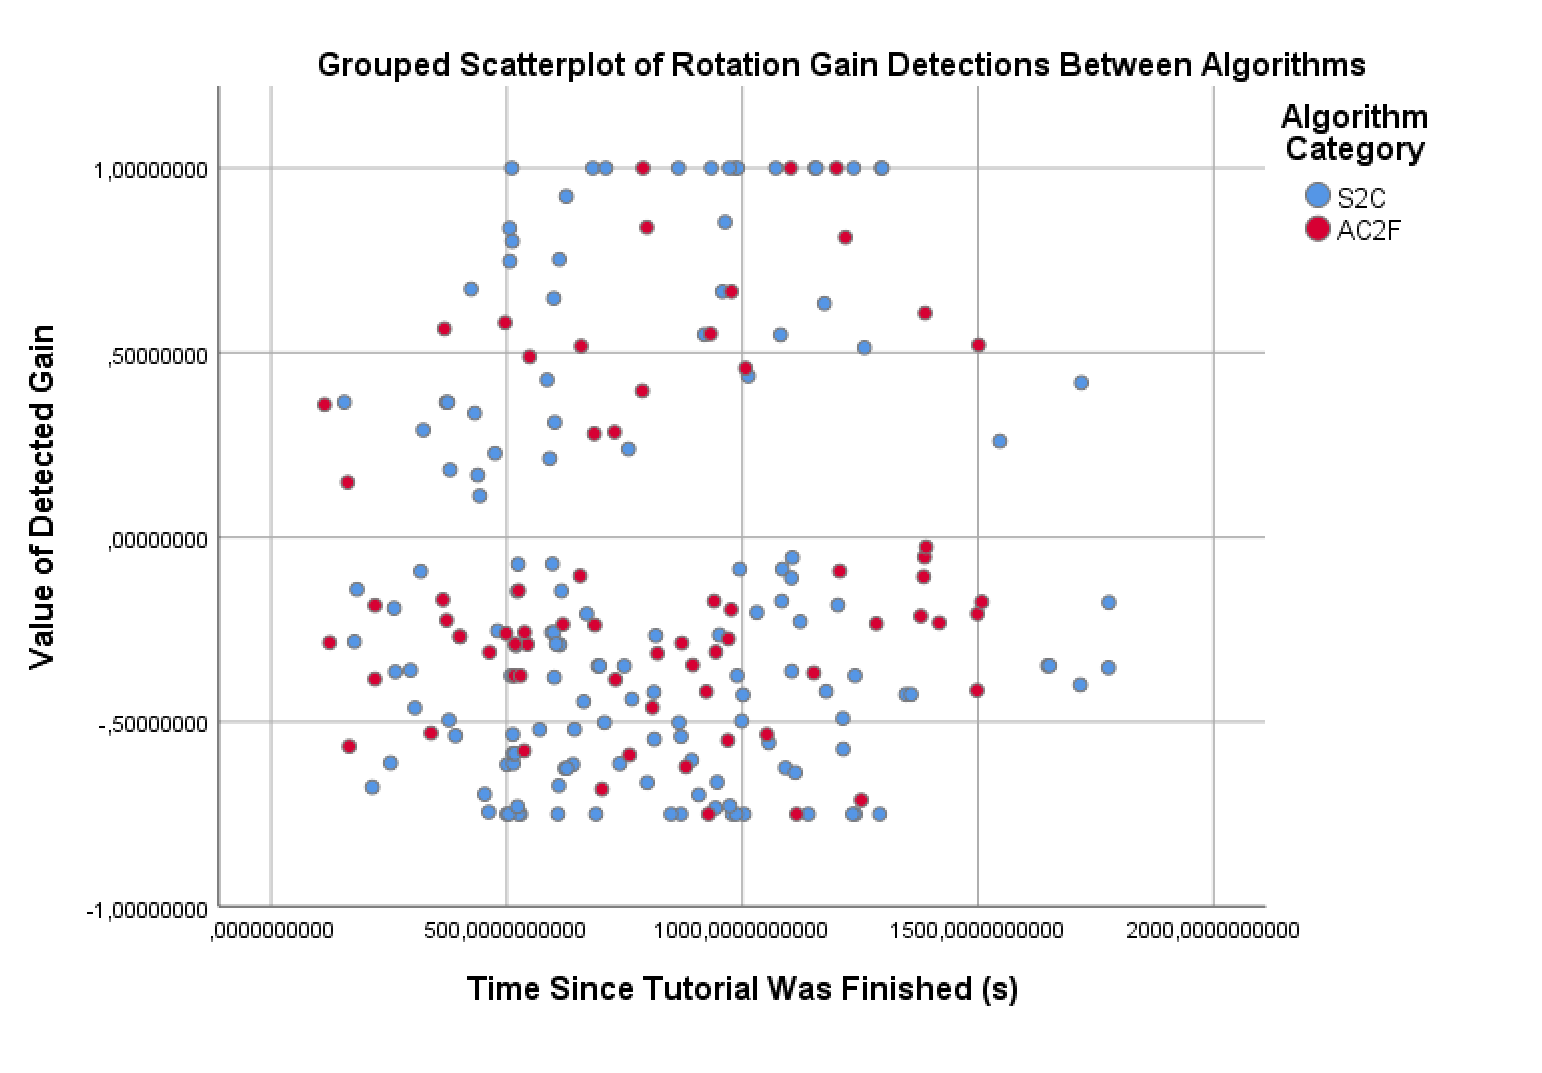
\includegraphics[width=0.75\textwidth]{figures/graphs/ProcessedRotationDetections.png}
    \caption[Finalised Detection Scatterplot For Rotation Gains, Grouped by Algorithm]{This scatterplot shows the finalised data of rotation gain detections and is grouped by algorithm.}
    \label{fig:rotationDetectionDataByAlgorithm}
\end{figure}

\begin{figure}[tbph]
    \centering
    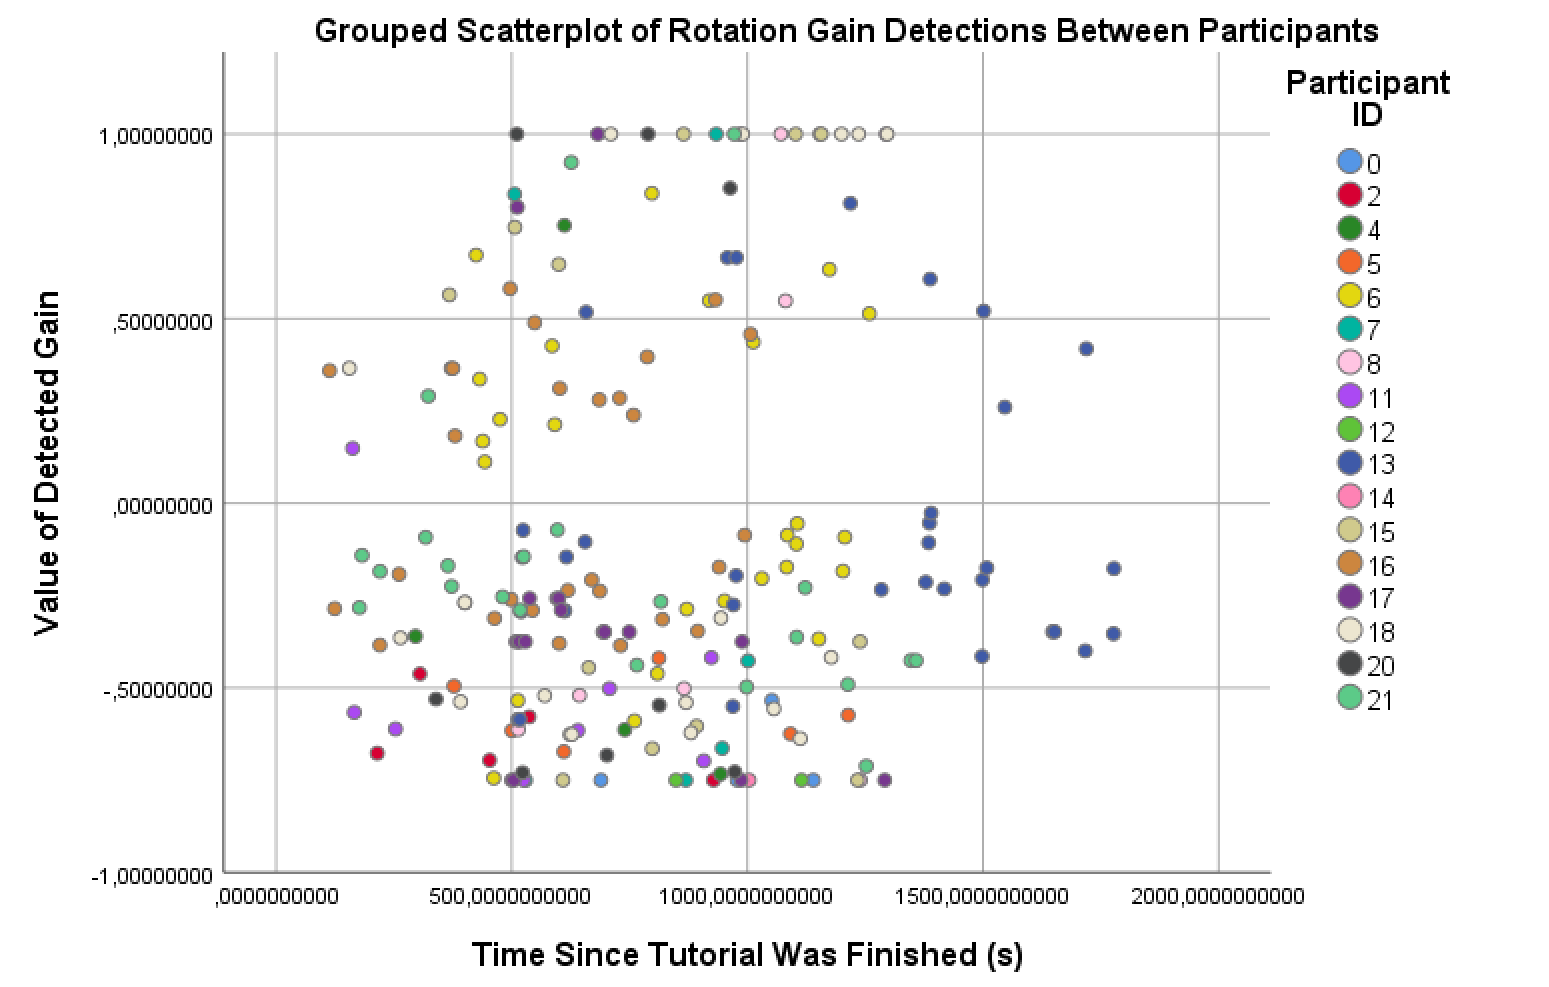
\includegraphics[width=0.75\textwidth]{figures/graphs/ProcessedRotationDetectionsByParticipant.png}
    \caption[Finalised Detection Scatterplot For Rotation Gains, Grouped by Participant ID]{This scatterplot shows the finalised data of rotation gain detections and is grouped by participant ID. Some ID's are not present as these participants did not notice any redirection or misunderstood the task they were given.}
    \label{fig:rotationDetectionDataByParticipant}
\end{figure}

\begin{figure}[tbph]
    \centering
    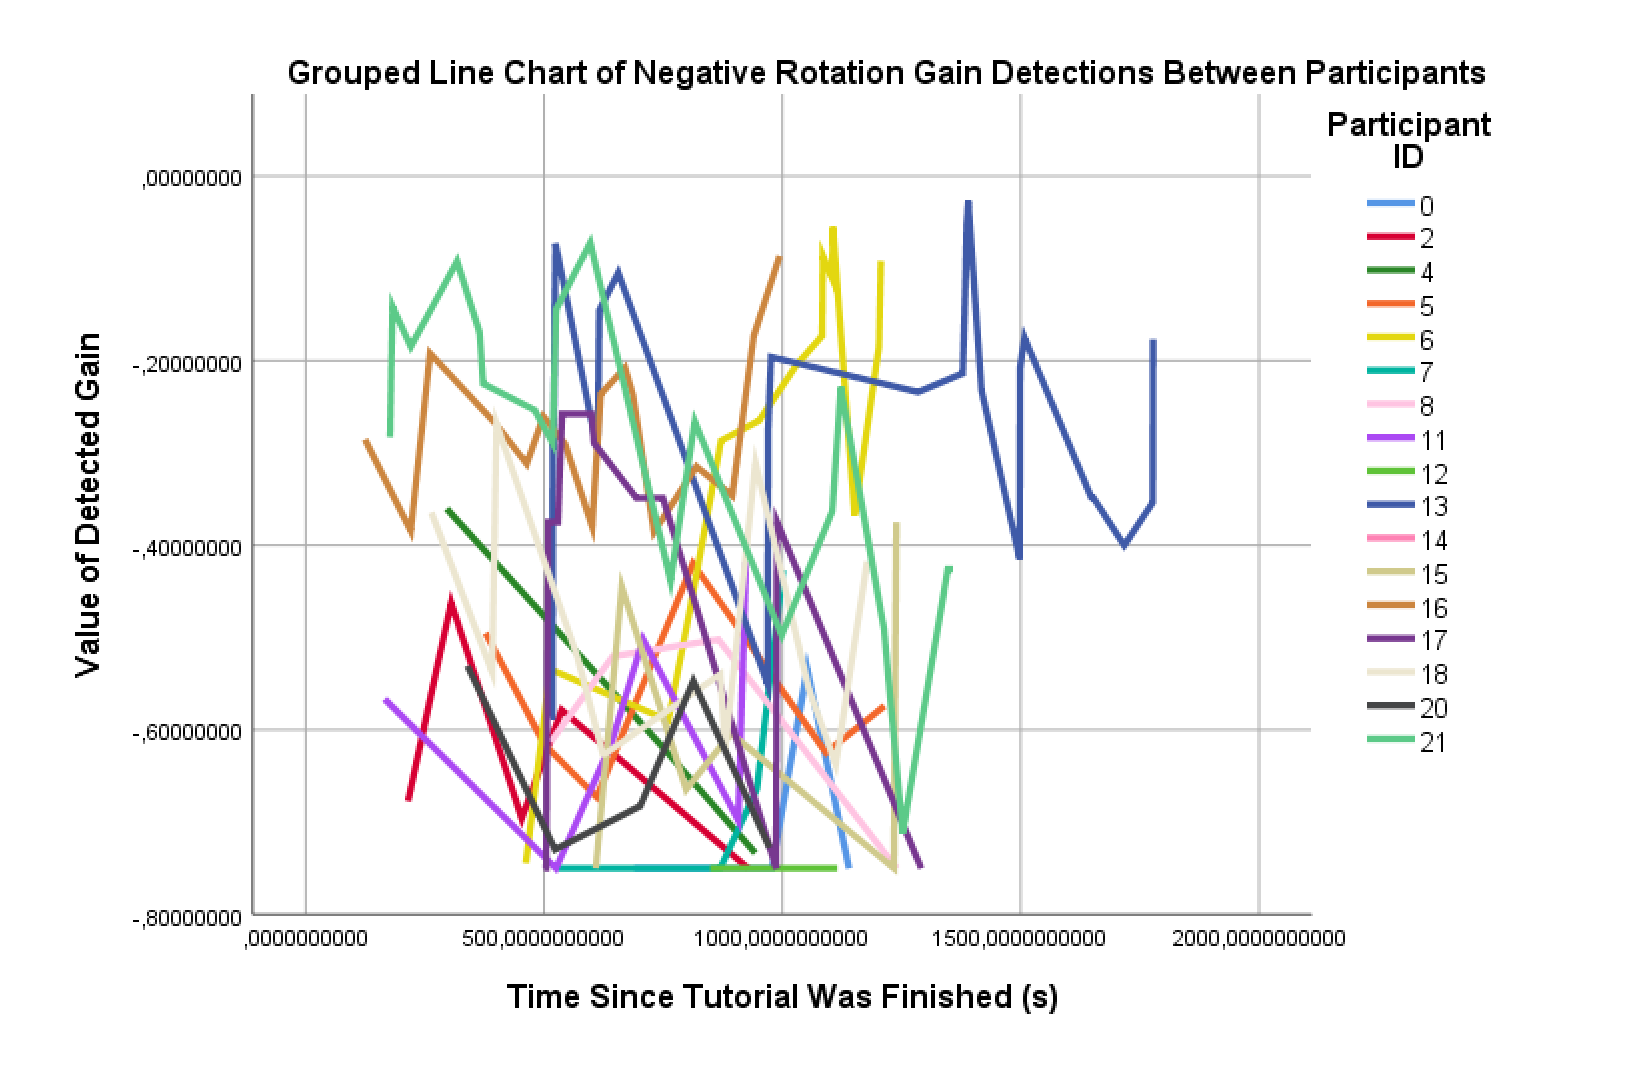
\includegraphics[width=0.75\textwidth]{figures/graphs/NegativeRotationDetectionsLineChart.png}
    \caption[Line Chart of Negative Rotation Gain Detections Between Participants]{This line chart shows the progression in negative rotation gain detections between participants.}
    \label{fig:negativeRotationDetectionLineChart}
\end{figure}

\begin{figure}[tbph]
    \centering
    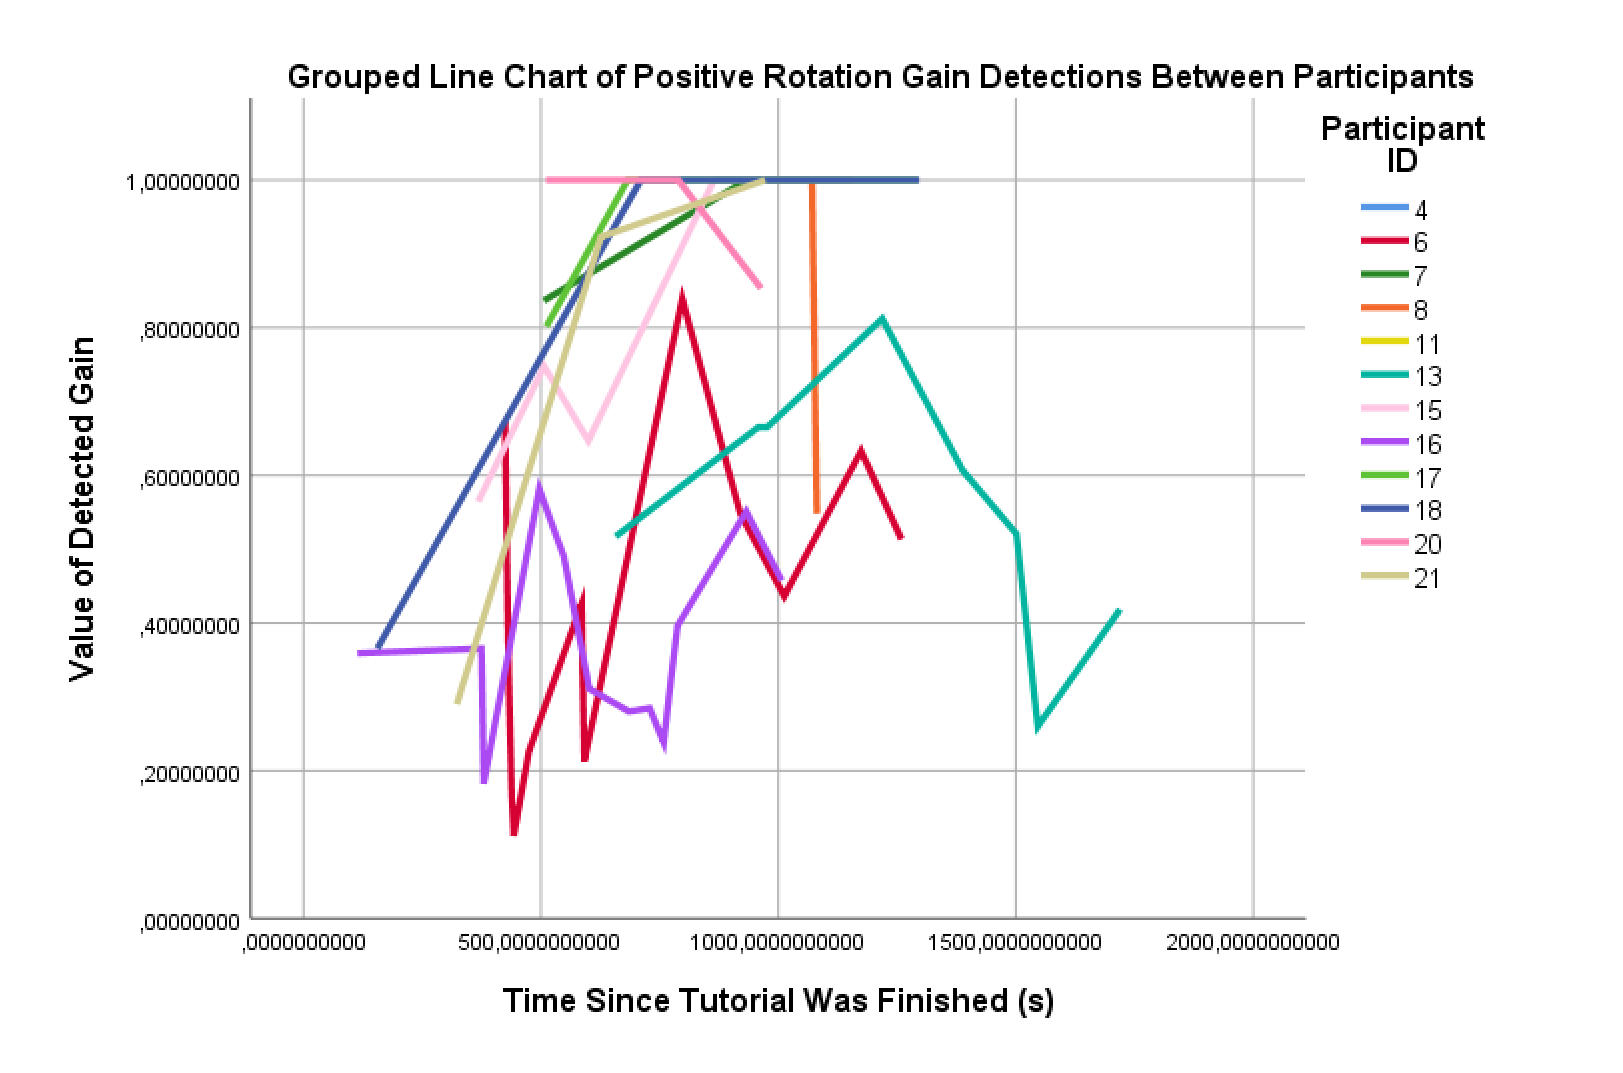
\includegraphics[width=0.75\textwidth]{figures/graphs/PositiveRotationDetectionsLineChart.png}
    \caption[Line Chart of Positive Rotation Gain Detections Between Participants]{This line chart shows the progression in positive rotation gain detections between participants.}
    \label{fig:positiveRotationDetectionLineChart}
\end{figure}

\begin{figure}[tbph]
    \centering
    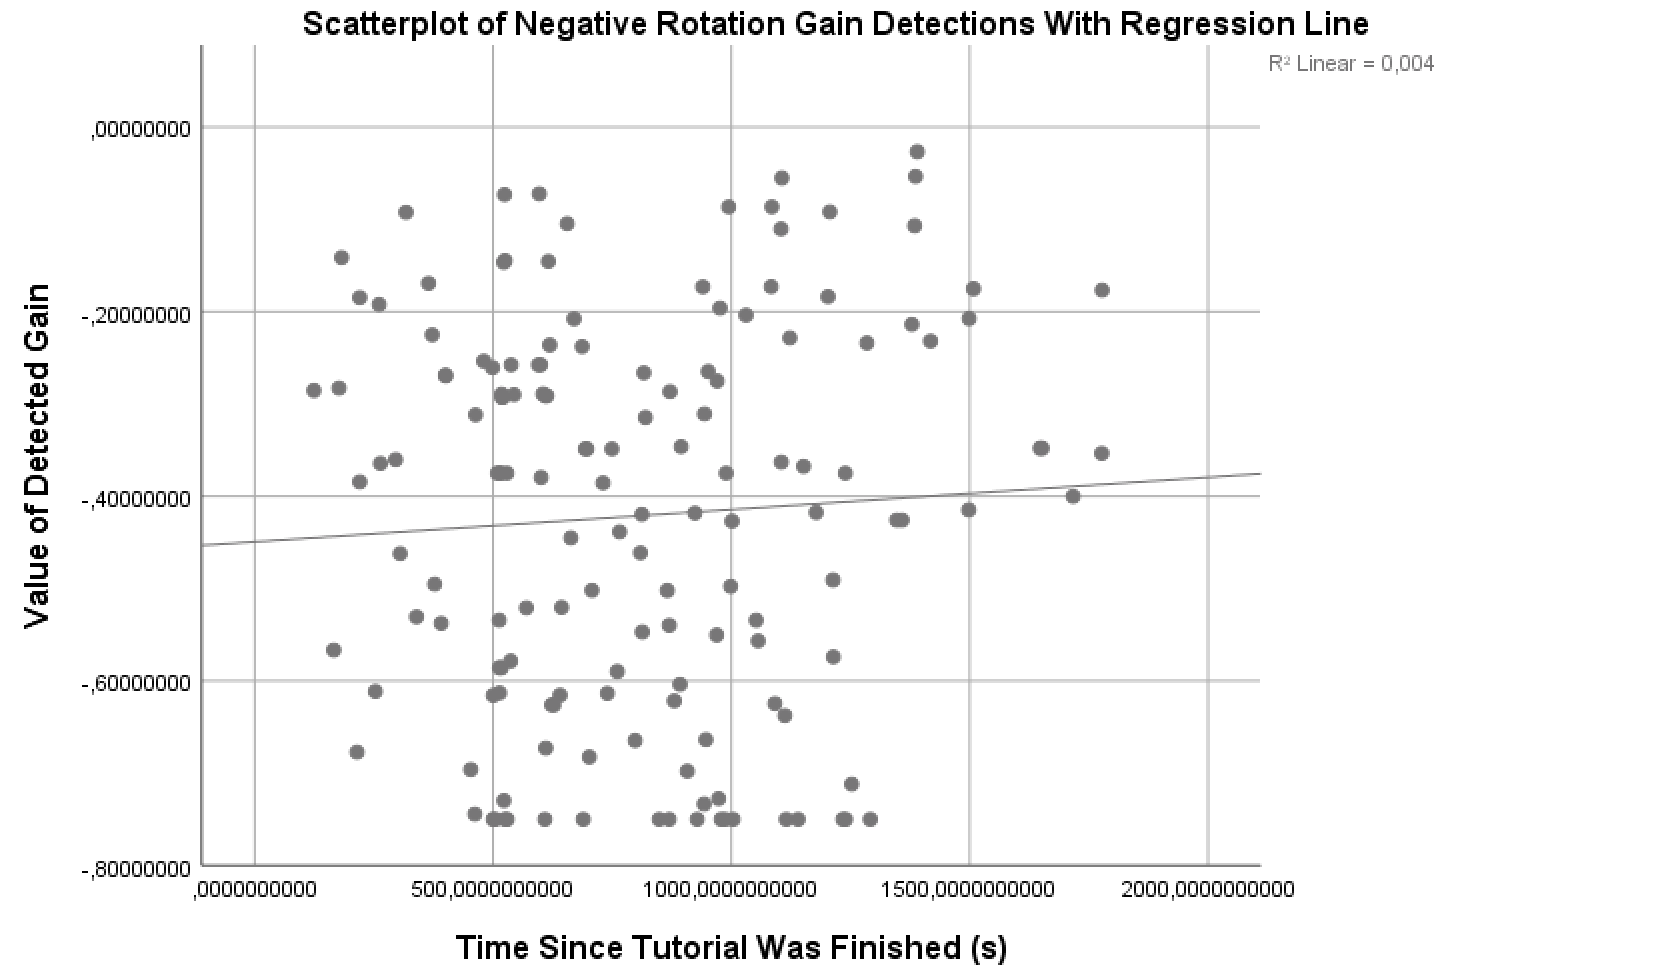
\includegraphics[width=0.75\textwidth]{figures/graphs/NegRotDetectionsRegLine.png}
    \caption[Scatterplot For Negative Rotation Gain Detections Including Regression Line]{This scatterplot shows the spread of negative rotation gain detections with an included regression line.}
    \label{fig:negRotRegLine}
\end{figure}

\begin{figure}[tbph]
    \centering
    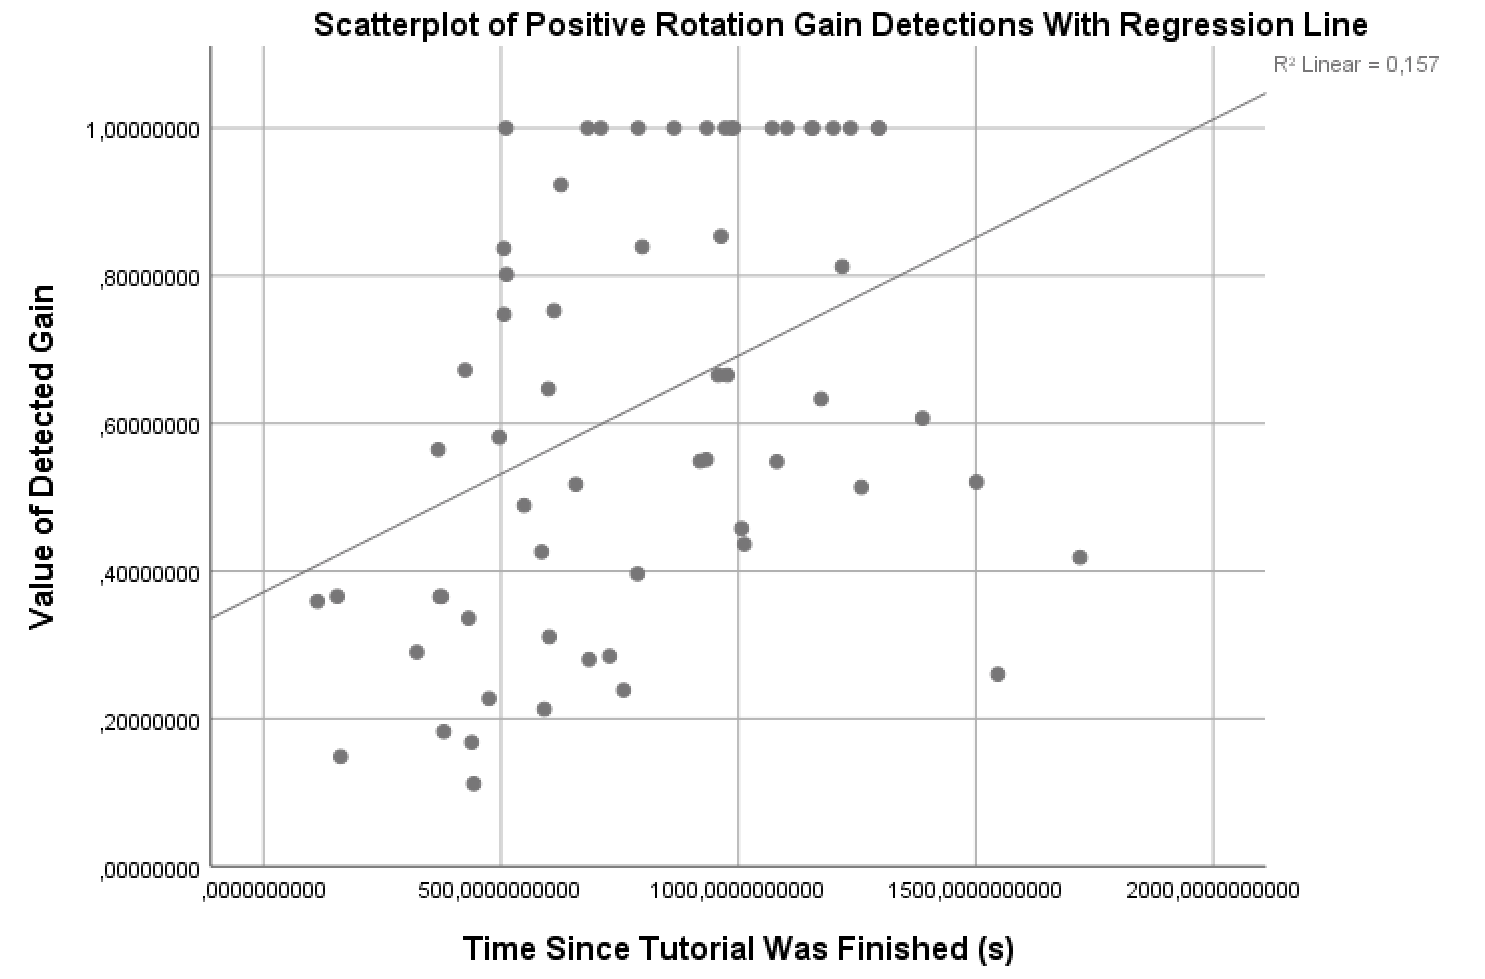
\includegraphics[width=0.75\textwidth]{figures/graphs/PosRotDetectionsRegLine.png}
    \caption[Scatterplot For Positive  Rotation Gain Detections Including Regression Line]{This scatterplot shows the spread of positive rotation gain detections with an included regression line.}
    \label{fig:posRotRegLine}
\end{figure}

\begin{figure}[tbph]
    \centering
    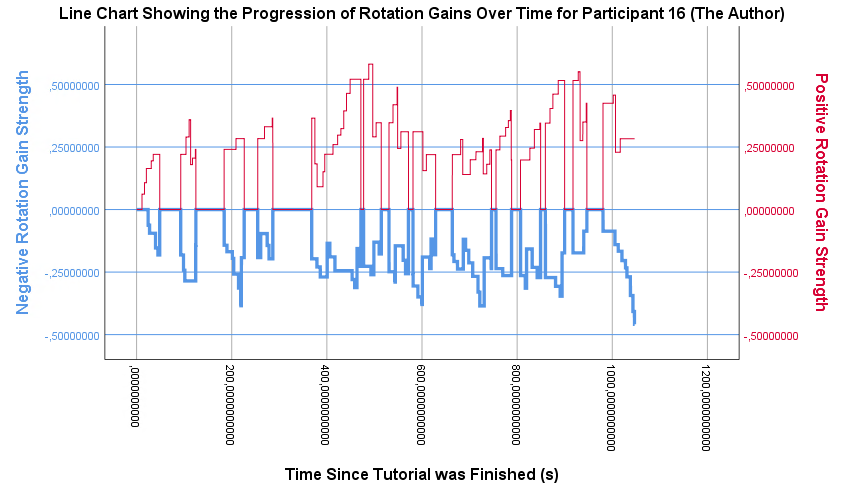
\includegraphics[width=0.75\textwidth]{figures/graphs/rotationGainProgressionAuthor.png}
    \caption[Line Chart Showing the Progression of Rotation Gains for Participant 16]{This line chart shows the progression of rotation gains over time for participant 16. Rotation gains gradually increase over time until they are detected, after which they are dropped by 50\%. Sections of time where gains are 0 are during distractor battles where the future virtual path has been aligned with the physical room centre.}
    \label{fig:authorRotationProgression}
\end{figure}

The post processing step which was mentioned in Section~\ref{sec:ex1postprocessing} resulted in 52 additional rotation gain detection events. This addition results in a total of 213 rotation gain detections throughout the entire sample. The processed data can be seen in Figure~\ref{fig:rotationDetectionDataByAlgorithm}, where it is grouped by algorithm and Figure~\ref{fig:rotationDetectionDataByParticipant}, where it is grouped by participant ID. To provide some additional visualisation, a line chart showing the progression of detections between participants can be seen in Figure~\ref{fig:negativeRotationDetectionLineChart} and Figure~\ref{fig:positiveRotationDetectionLineChart}.

 A figure illustrating the incremental progression of rotation gains over time for participant 16 (the author) can be seen in Figure~\ref{fig:authorRotationProgression}. Finally, individual scatterplots for negative/positive rotation gain detections with an included regression line can be found in Figure~\ref{fig:negRotRegLine} and Figure~\ref{fig:posRotRegLine}. It should be noted that some participants are not shown in these graphs as they did not provide any detection events. 

\subsection{Curvature Detections}
\begin{figure}[tbph]
    \centering
    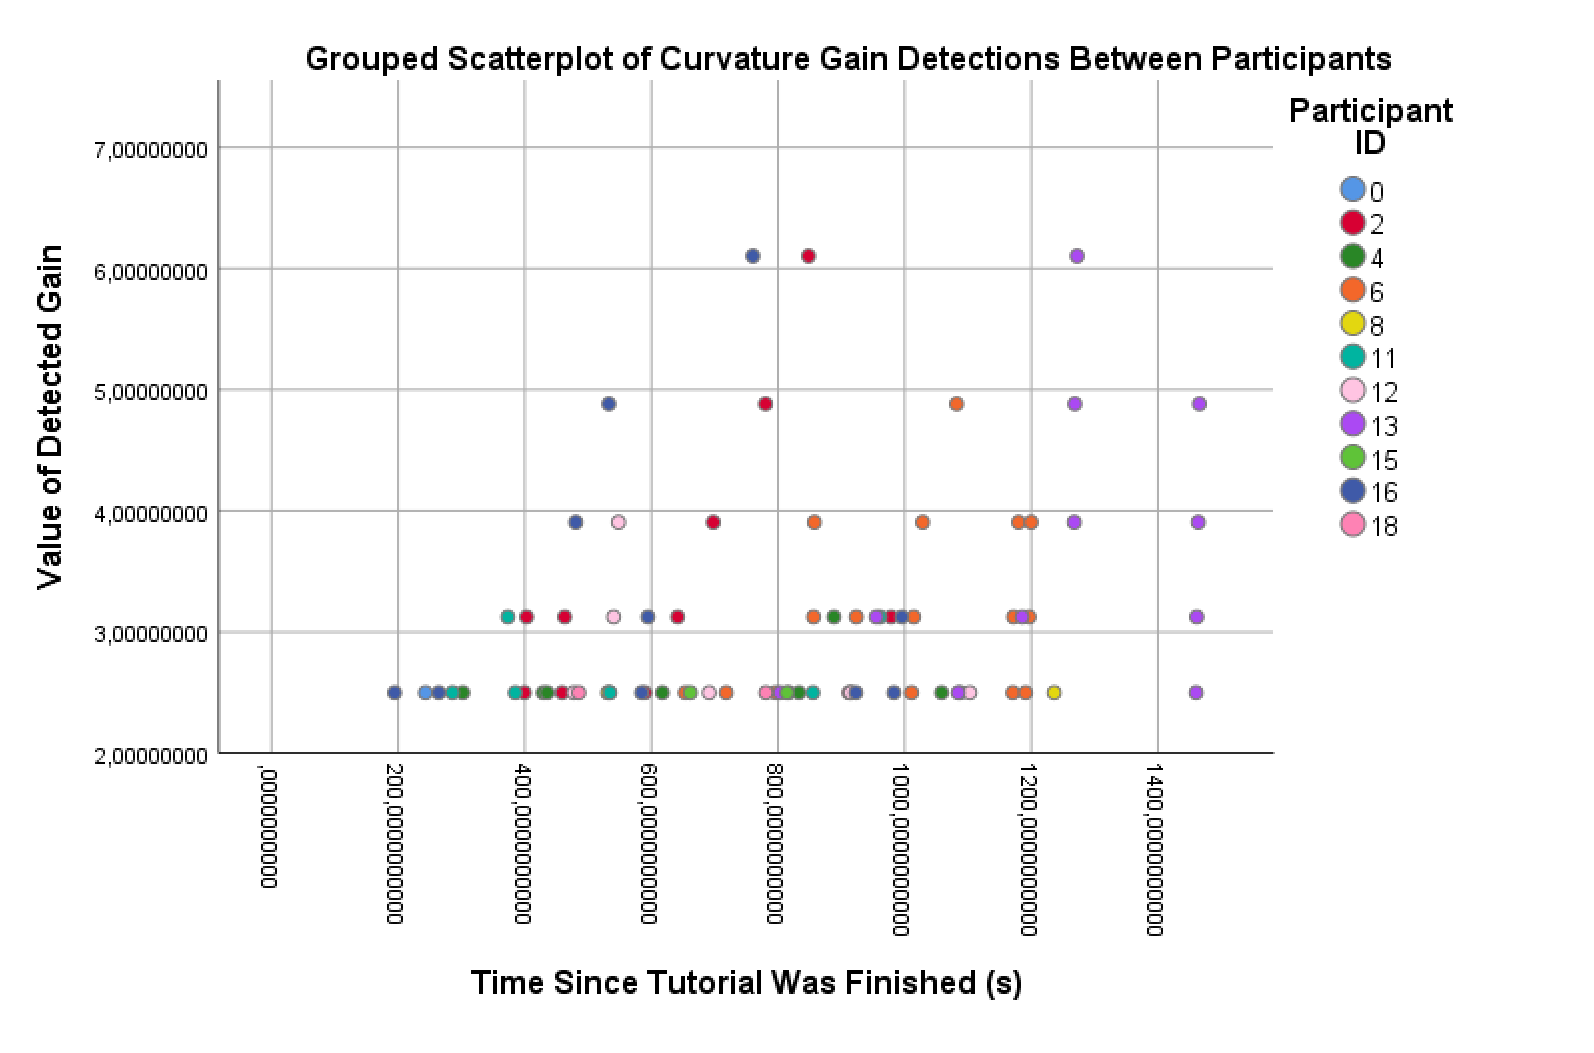
\includegraphics[width=0.75\textwidth]{figures/graphs/CurvatureDetectionScatter.png}
    \caption[Finalised Detection Scatterplot For Curvature Gains, Grouped by Participant ID]{This scatterplot shows the finalised data of curvature gain detections and is grouped by participant ID. Curvature values in this case are defined as the radius of the curvature arc.}
    \label{fig:curvatureDetectionData}
\end{figure}

The various curvature gain detection events that happened during the walking phase of Ensemble Retriever can be seen in Figure~\ref{fig:curvatureDetectionData}.

\subsection{Mean Detection Thresholds}
\begin{table}[!h]
\centering
\begin{tabularx}{\textwidth}{|X|S|X|}
\hline
Type of Gain & {Mean Detection Threshold} & N (Total Number of Detections) \\
\hline
S2C: Positive Rotation Gain & 0.6479 & N = 43 \\
\hline
S2C: Negative Rotation Gain & -0.4631 & N = 101 \\
\hline
AC2F: Positive Rotation Gain & 0.5828 & N = 19 \\
\hline
AC2F: Negative Rotation Gain & -0.3365 & N = 50 \\
\hline
S2C+AC2F: Positive Rotation Gain & 0.6279 & N = 43+19 \\
\hline
S2C+AC2F: Negative Rotation Gain & -0.4212 & N = 101+50 \\
\hline
S2C: Curvature Radius & 3.0978m & N = 78 \\
\hline
\end{tabularx}
\caption[Experiment 1: Mean Detection Thresholds]{This table shows the various detection thresholds that were calculated as the mean of all detection events in each respective category.}
\label{table:ex1DetectionThresholds}
\end{table}

The aggregated mean detection thresholds which have been generated out of the previously presented data can be seen in Table~\ref{table:ex1DetectionThresholds}. 

\subsection{Test for Normality and Choice of Significance Test}
Before performing any statistical significance tests on the data, it is first necessary to test the normality of it. For this, the Shapiro-Wilk test was used on positive and negative rotation gain detections. There is no possibility to compare different conditions for curvature gains, and as such, no normality test was performed on this data. 

\subsubsection{Positive Rotation Gain Detection Normality}
The Shapiro-Wilk test resulted in $p < 0.001$ for the S2C category and $p = 0.295$ for the AC2F counterpart. The S2C category is thus not normally distributed while AC2F is. 

\subsubsection{Negative Rotation Gain Detection Normality}
The Shapiro-Wilk test resulted in $p < 0.001$ for the S2C category and $p = 0.015$ for AC2F. Both of these are thus not normally distributed.  

\subsubsection{Choice of Significance Test}
Since the data is not normally distributed, it is not possible to use standard tests like the independent samples t-test. Instead, the Mann-Whitney U non-parametric test is used as it does not have the same assumption of normally distributed data. 
   
\subsection{Hypothesis Testing}
Before performing the Mann-Whitney U test, it is first necessary to determine whether the shapes of the data between conditions is similar or not. 
\subsubsection{Mann-Whitney U Shape Test}
\begin{figure}[tbph]
    \centering
    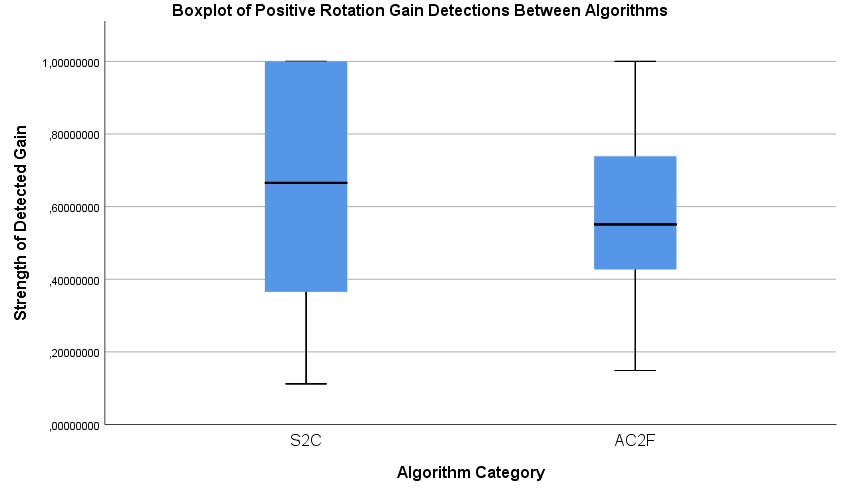
\includegraphics[width=0.75\textwidth]{figures/graphs/PosRotationDetectionBoxplot.png}
    \caption[Boxplot on Positive Rotation Detections in Experiment 1]{This boxplot shows the spread of detected gains between algorithms for positive rotation gains in Experiment 1.}
    \label{fig:posRotEx1Boxplot}
\end{figure}

\begin{figure}[tbph]
    \centering
    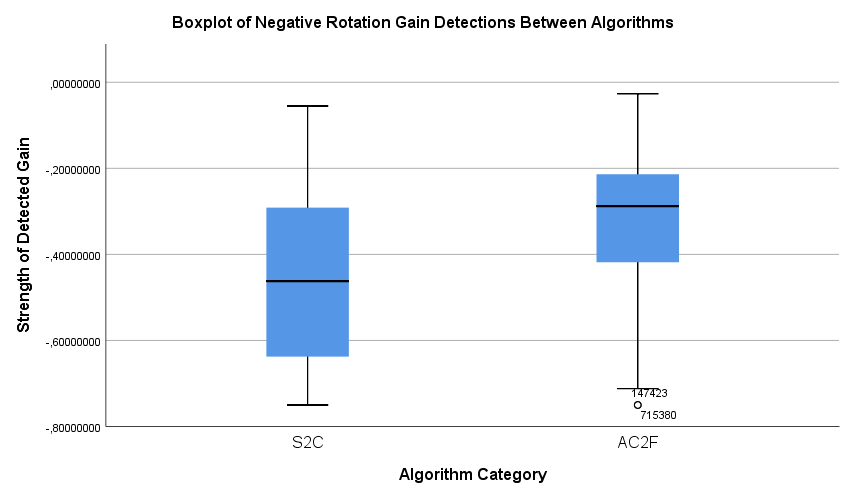
\includegraphics[width=0.75\textwidth]{figures/graphs/NegRotationDetectionBoxplot.png}
    \caption[Boxplot on Negative Rotation Detections in Experiment 1]{This boxplot shows the spread of detected gains between algorithms for negative rotation gains in Experiment 1.}
    \label{fig:negRotEx1Boxplot}
\end{figure}

The shapes of the data can be seen in Figure~\ref{fig:posRotEx1Boxplot} and~\ref{fig:negRotEx1Boxplot}. In general, it does not seem as if the shape between the conditions is similar enough in either of the cases. As such, the Mann-Whitney U comparison will be on mean ranks. It should also be noted that the Mann-Whitney U test does have an assumption of independent observations that cannot be fulfilled due to the within-subjects design of the experiment.

\subsubsection{Mann-Whitney U Results}
The results of the Mann-Whitney U provided a value of $U = 362.5, p = 0.478$ between S2C and AC2F conditions for positive rotation gains. This means that there are no significant differences between the states for these gains. For negative rotation gains, the statistical test resulted in $U = 1639, p < 0.001$, meaning that it is significantly harder to notice negative rotation gains in the walking state in Ensemble Retriever.

\subsection{Demographic Insights}
\begin{figure}[tbph]
    \centering
    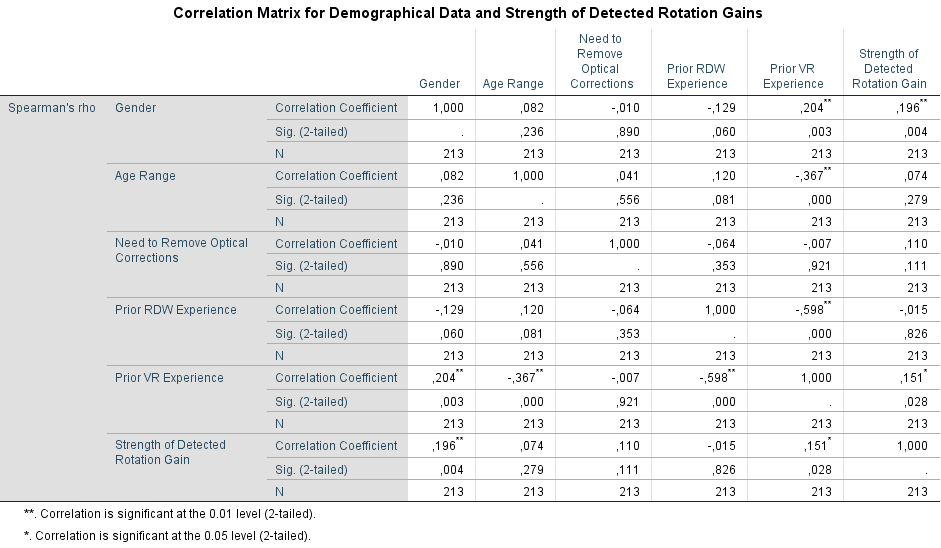
\includegraphics[width=0.8\textwidth]{figures/graphs/DemographicalCorrelationsEx1.png}
    \caption[Experiment 1 Demographic Correlation Matrix]{Correlation matrix for the demographic data in Experiment 1 and the rotation gains that were detected. N values are 213 as there were 213 rotation gain detections.}
    \label{fig:ex1demogcorrelationmatrix}
\end{figure}

In order to look for demographic insights, a correlation analysis has been conducted. This analysis focuses on rotation gain detections and makes use of the Spearman's Rho correlation test as the detection data is not fully normally distributed. The correlation matrix can be seen in Figure~\ref{fig:ex1demogcorrelationmatrix}. The most interesting among these correlations is the positive correlation between prior VR experience and the strength of detected gains. As such, a deeper analysis has been conducted on this correlation to look for insights. 

\subsubsection{Prior VR Experience and Rotation Gain Detections}
\begin{figure}[tbph]
    \centering
    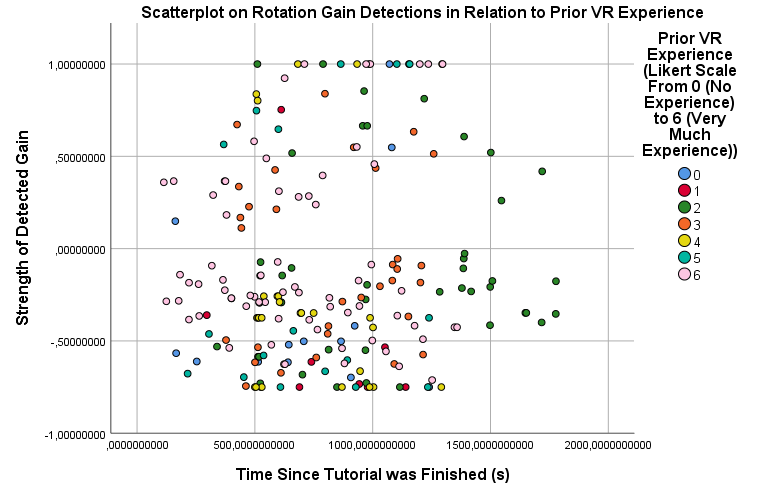
\includegraphics[width=0.75\textwidth]{figures/graphs/PriorVRExperienceDetectionScatter.png}
    \caption[Scatterplot on Rotation Gain Detections in Relation to Prior VR Experience]{This scatterplot shows the rotation gains that were detected in Experiment 1 and their relation to prior VR experience.}
    \label{fig:rotationGainDetectionScatterVRExperience}
\end{figure}

\begin{figure}[tbph]
    \centering
    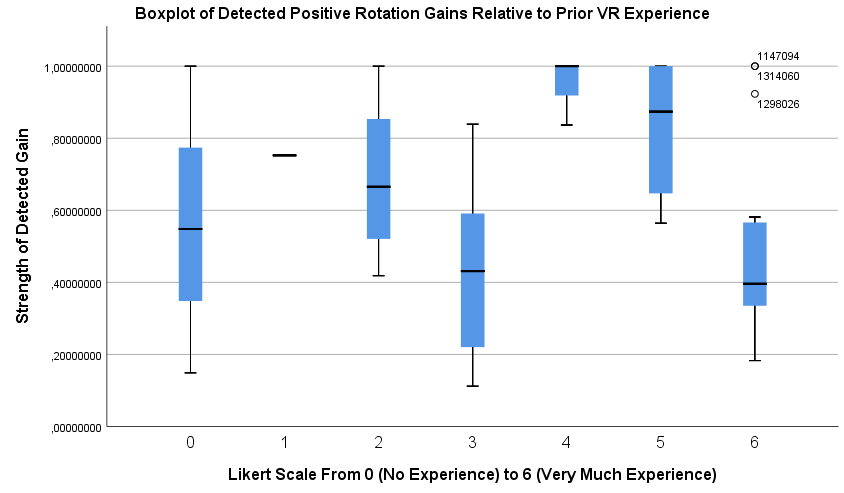
\includegraphics[width=0.75\textwidth]{figures/graphs/PosRotDetectionsByVRExperience.png}
    \caption[Boxplot on Detected Positive Rotation Gains by VR Experience]{This boxplot shows the spread of detected positive rotation gains in relation to prior VR experience.}
    \label{fig:posRotDetectionBoxplotVRExperience}
\end{figure}

\begin{figure}[tbph]
    \centering
    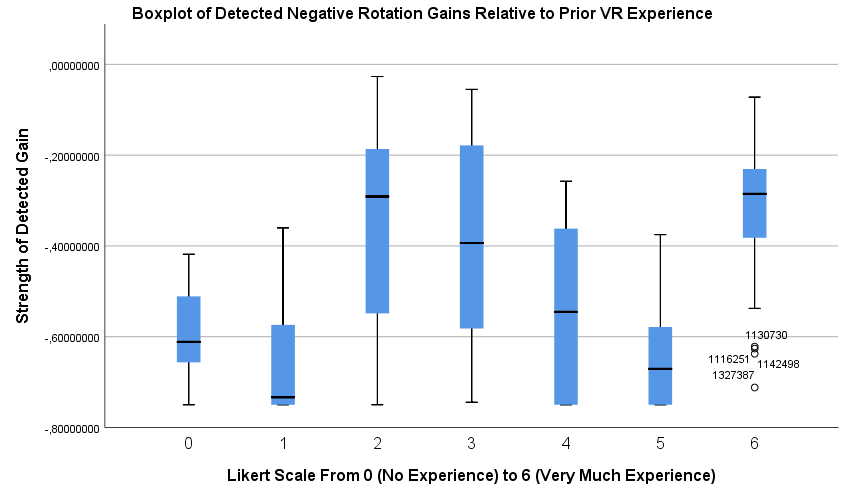
\includegraphics[width=0.75\textwidth]{figures/graphs/NegRotDetectionsByVRExperience.png}
    \caption[Boxplot on Detected Negative Rotation Gains by VR Experience]{This boxplot shows the spread of detected negative rotation gains in relation to prior VR experience.}
    \label{fig:negRotDetectionBoxplotVRExperience}
\end{figure}

A scatterplot on the strength of rotation gain detections in relation to prior VR experience can be seen in Figure~\ref{fig:rotationGainDetectionScatterVRExperience}. Boxplots for positive and negative gains can be seen in Figure~\ref{fig:posRotDetectionBoxplotVRExperience} and~\ref{fig:negRotDetectionBoxplotVRExperience}.


\subsubsection{Qualitative Feedback}
The participants also provided some written qualitative feedback through the post-test questionnaire. This section summarises the feedback that was provided on a question by question basis. 

\paragraph{Whether the Participants Found Any Bugs or Glitches}
Some participants experienced minor controller tracking problems when standing in certain areas of the physical tracking space. These were quickly resolved by holding their controllers up in the air. 

\paragraph{Whether the Participants Found the Experience Enjoyable}
In general, participants found the experience to be very positive. Despite this, some mentioned that the experience was rather long, so fighting the same distractors over and over got a bit annoying towards the end.

\paragraph{How the Participants Felt About the Redirection Techniques}
When noticed, participants mentioned that the redirection felt rather odd initially. After a while, some participants got used to the effect and found it to be effective while others mentioned it was a bit awkward and annoying. 

\paragraph{Whether the Participants Had Any Problems Throughout Their Experience}
In general, participants mentioned that it was rather frustrating to untangle themselves from the HMD cable as they played. Three participants also mentioned that they experienced a mild amount of discomfort due to the redirection, but that they did not feel like it was enough to mention during the experiment. 

\paragraph{Additional Comments From Participants}
Other than the already mentioned feedback, participants did provide some additional comments on how they felt the experience could be improved. The majority of this feedback has been kept in mind when making changes for Experiment 2. In particular, participants wanted some of the distractors to fire slightly faster projectiles as some of the slower ones became a bit boring over time. The full list of software changes between Experiment 1 and 2 can be seen in Section~\ref{sec:changesBetweenExperiments}.

\subsection{Summary}
\begin{table}[h!]
\centering
\scalebox{0.9}{
\begin{tabularx}{\textwidth}{|X|X|}
\hline
Variable & Context \\
\hline
Size + Shape of Physical Tracking Space & 5m x 5.75m rectangle \\
\hline
Optical Flow/Visual Density in VE & Low Poly Artstyle. Limited visual density outside of environmental trees and shining mushrooms. The walkable environment is fully open. The player has to fight enemy distractors while exploring which move around the player and shoot various salient projectiles that might contribute to increased optical flow and visual density. See figures in Chapter~\ref{chap:implementation} for examples.\\
\hline
Hardware: HMD Field of View & HTC Vive. ~145 diagonal degrees FoV. \\
\hline
Speed of Walking & \textasciitilde$0.2576$ $m/s$ on average (Total distance travelled / Total time spent walking between participants). Static curvature gains employed. \\
\hline
Engagement/Distraction & The participants played through a VR game which consisted of walking around, collecting clues (working memory task) and fighting enemy distractors while exploring. Overall engagement levels based on feedback and observation of participants could be considered as high. \\
\hline
Awareness of Redirection & Participants were informed of redirection and the basics of redirected walking. The concept of distractors was not directly explained, but mentioned in the information/consent sheet. \\
\hline
Gender & 20M, 2F (One among the 22 participants was excluded from the data analysis)\\
\hline
Estimation Method & Incrementally and randomly increasing one gain at random timesteps. Rotation gain is halved when detected, curvature radius is multiplied by 25\% when detected. \\
\hline
Adaptation: Curvature Gains & The experiment employed an incremental gains method for estimation. Gains would as such, gradually increase over time. Some adaptation could be possible, but the curvature detection data cannot answer this. \\
\hline
Adaptation: Positive Rotation Gains & The data does appear to point towards a potential adaptation towards positive rotation gains. The variability of negative rotation gain detections makes it hard to say whether this also is true for these. \\
\hline
Prior VR Experience & While relatively hard to directly conclude with the current data sample, participants with the highest amount of VR experience were the most sensitive towards redirection. Those with no prior VR experience were among the least sensitive. It should also be noted that some participants who had no prior VR experience could not detect any redirection as well. \\
\hline
\end{tabularx}}
\caption[Experiment 1: Summary Over Contextual Variables in Relation To Detection Thresholds]{Summary of variables from Chapter~\ref{chap:relatedWork} with some additions and how Experiment 1 relates to these.}
\label{table:ex1VariableSummary}
\end{table}

A contextual summary of how the various variables from Chapter~\ref{chap:relatedWork} relate to this experiment can be found in Table~\ref{table:ex1VariableSummary}. It also includes some potentially new and relevant variables based on the results that have been shown. In general, the results showed that negative rotation gains are significantly easier to detect during battles (Mann-Whitney U: $U = 1639, p < 0.001$), compared to when walking around. No significant difference could be found for positive rotation gains between the walking and battle states (Mann-Whitney U: $U = 362.5, p = 0.478$). 
\section{Discussion}

\todo{Look through experiment 1 notes in general for various insights and topics that can be discussed. Expect a good amount of discussion around the results and speculation on why they ended up as they did}

\subsection{Curvature Gain Detection Patterns}
* When noticed the player clicks several times until they stop noticing it. This creates the fairly rigid ladders of detection data as one participant continually presses and decreases the strength at a set rate from the minimum. 

\subsection{Redirection Adaptability}
* Will probably be relevant to discuss
* Boelling et al. mentions there is some adaptivity effect at least for curvature gains. They would expect this to be true for other gains as well
* Do we see an adaptivity effect or not?
   * If no, it is likely that the alignment phases during AC2F limit adaptivity effects as gains are disabled at those times.
* The estimation method may play a role
* At the same time, once aligned AC2F disables gains completely, allowing the user to get used to normal head rotations again. This could counteract adaptivity effects

\subsection{Individual detection thresholds}
* Might be relevant to discuss
* Creating calibrating scenarios in software that allows users to estimate their own thresholds

\subsection{Large variability in detections}
* Can be many reasons for this
* One limitation is users looking left and right repeatedly makes them notice that they are being redirected
* S2C dampening helps with this after finishing a distractor, AC2F does not have an equivalent at the present as you need most of the redirection initially, then it is turned off once aligned


* There is definitely far less positive detections that negative ones, positive rot threshold is a tiny bit higher too (I think?)

\subsection{Participant Feedback on Pause - Turn - Centre}
* Generally positive
* It felt natural and easy to use
* Some mentioned that it took a little bit time to get used to though

\subsection{Comparing The Results With Fuglestad's Study}
\todo{Compare the difference in DT's between Bjørn's incremental and standard experiments. Argue that while the estimation method likely has an effect, so does the fact that users were distracted while performing the incremental experiment.}

\subsection{Limitations of using Gain Caps}
\chapter{Experiment 2: Effectiveness of Distractors}
This chapter consists of the Method, Results and Discussion components for Experiment 2. The experiment itself focuses on various effectiveness metrics for the developed redirected walking solution. 

\todo{Make sure the structure is somewhat similar between ex1 and ex2}

\section{Method}
As part of developing the extension to the redirected walking toolkit, one of the implemented components was the AC2F algorithm. Since AC2F makes use of more predictive information compared to S2C, it would be interesting to see whether this provides a more effective solution when using distractors. As such, this experiment compares two different conditions. The first makes use of S2C only throughout an entire playthrough of Ensemble Retriever while the other uses S2C during walking and AC2F during the standing distractor battles. The redirection gains employed in this experiment are derived from the estimated thresholds in Chapter~\ref{chap:ex1}. This playthrough of Ensemble Retriever is also somewhat shorter than in Experiment 1, taking roughly 15-20 minutes instead of \textasciitilde30 minutes in hopes that it would make it easier to gather participants. 

This section consists of the related methods that have been used to measure and test the effectiveness of employing AC2F when using distractors. 

\subsection{Hypotheses}
In order to test effectiveness, it is first necessary to operationalise the term. For this experiment there are two primary types of effectiveness that have been focused on. The first of these is Azmandian et al.'s relative effectiveness~\cite{azmandian2015physical}. Relative effectiveness provides a measurement of redirection effectiveness through the number of resets that happen throughout one condition compared to another. It is defined with the following formula:
$$
RelativeEffectiveness_{Algorithm} = \frac{ResetCount_{ControlCondition} - ResetCount_{ExperimentalCondition}}{ResetCount_{ControlCondition}}
$$
This results in the percentage difference of the experimental condition compared to the control counterpart. 

The second effectiveness metric that this experiment focuses on is effectiveness in terms of the time in seconds it takes for the user's future path to be aligned to the centre of the room. The distractor solution is in general agnostic to the redirection algorithm that is employed and simply disables any redirection whenever the future virtual path is aligned with the physical centre. This means that it is simple to compare S2C and AC2F for this effectiveness metric.

Given the two effectiveness metrics that the experiment focuses on, two null hypotheses have been established:
\begin{description}
  \item[$H_{0_1}$:] Employing S2C+AC2F in Ensemble Retriever does not provide significantly better relative effectiveness compared to S2C only. 
  \item[$H_{0_2}$:] Employing S2C+AC2F in Ensemble Retriever does not result in significantly lower time needed to align the user's future path towards the centre of the room compared to S2C only.
\end{description}


\subsection{Data Collection}
Experiment 2 employs a similar data collection procedure to Experiment 1. It records data every frame that Ensemble Retriever is running and focuses on recording data that is relevant to the two established null hypotheses. Some of these include data on when and how many resets that have been triggered, how much time it takes to be aligned with the centre of the room and the time it takes to defeat a distractor. A full list with descriptions for each piece of recorded data can be found in Section~\ref{sec:ex2dataformat}. 

\subsection{Data Post Processing}\label{sec:ex2postprocessing}
One problem that can affect the results for testing both hypotheses is what could be considered as ''unintentional resets''. These are resets that can happen during distractor battles in two different ways:
\begin{enumerate}
    \item If the user is walking fast enough, the buffer between a distractor triggering and a reset triggering might be too small. By the time the user stops after triggering a distractor, they have reached the boundary for triggering a reset as well. This means that the user is almost instantly aligned to the physical centre. 
    \item If the user moves around a lot during battles they risk triggering a reset since they already are close to the physical bounds while fighting. 
\end{enumerate}

Both of these cases could be considered as resets that are unintentional and would skew the results. In terms of frequency, it is the first of these cases that was the most apparent from observation of participants as they played. As such, a data processing step was conducted to attempt removing as many of these unintentional resets as possible. 

In terms of removing unintentional resets, there are two potential options. The first of these is to simply not include any resets that happen during battles with distractors. This is the simple solution, but may not end up including legitimate resets that happen between the start and end of a distractor's death animation. A distractor is considered as inactive after this death animation has finished. There are cases where participants start to walk right as a distractor's death animation starts which means that this method is not ideal as it may miss resets that happen in this time range. 

The second option is to discard any resets that happen within a given time buffer from when a distractor spawns. This is harder from a post processing perspective, but should provide more accurate results. This means that it can include the legitimate resets that may happen at the end of a distractor's life cycle while minimising the amount of unintentional resets. 
In order to decide the length of this time buffer it is first necessary to understand the minimum time a distractor battle has taken. For the recorded data in this experiment, the minimum time was \textasciitilde18.23 seconds. Since this time is recorded at the end of a distractor's death animation it is necessary to provide some buffer so that legitimate resets can be identified.

Given the minimum distractor duration of 18.28 seconds and the need for some buffer, the post processing uses a time of 10 seconds. This means that any resets that happened within the first 10 seconds of a distractor spawning become discarded from the analysis. A walkthrough for the entire post processing procedure can be found in Section~\ref{sec:ex2postprocessingdetails}.

\subsubsection{Adding Penalties for Failed Alignments}
One element that may differ between algorithms is the rate of failed alignments. Failed alignments are in this case defined as the failure to align the user's future virtual path to the centre of the physical room throughout the lifetime of a distractor. Given that these failure cases may be different between the two conditions it is necessary to factor them into the hypothesis testing in some way. For this thesis, the problem is handled by providing a time penalty whenever an algorithm fails to align the user properly when testing $H_{0_2}$. This way, each spawned distractor results in either a successful or unsuccessful alignment time which can be factored into the data analysis. The value for the time penalty is chosen to be the average time needed to defeat a distractor, which in this case was 54.86 seconds. The reasoning for choosing the average time needed to defeat a distractor is that average successful alignment times primarily were within the scope of \textasciitilde23 seconds. The average time taken to defeat a distractor is thus sizeably different compared to the successful alignment times and should provide a reasonable skew in the data if there is a large difference in fail rates. 

\todo{Is the argumentation for using the average as penalty good enough?}

\subsection{Changes in Experiment Environment}\label{sec:ex2environmentchanges}
\begin{figure}[tbph]
    \centering
    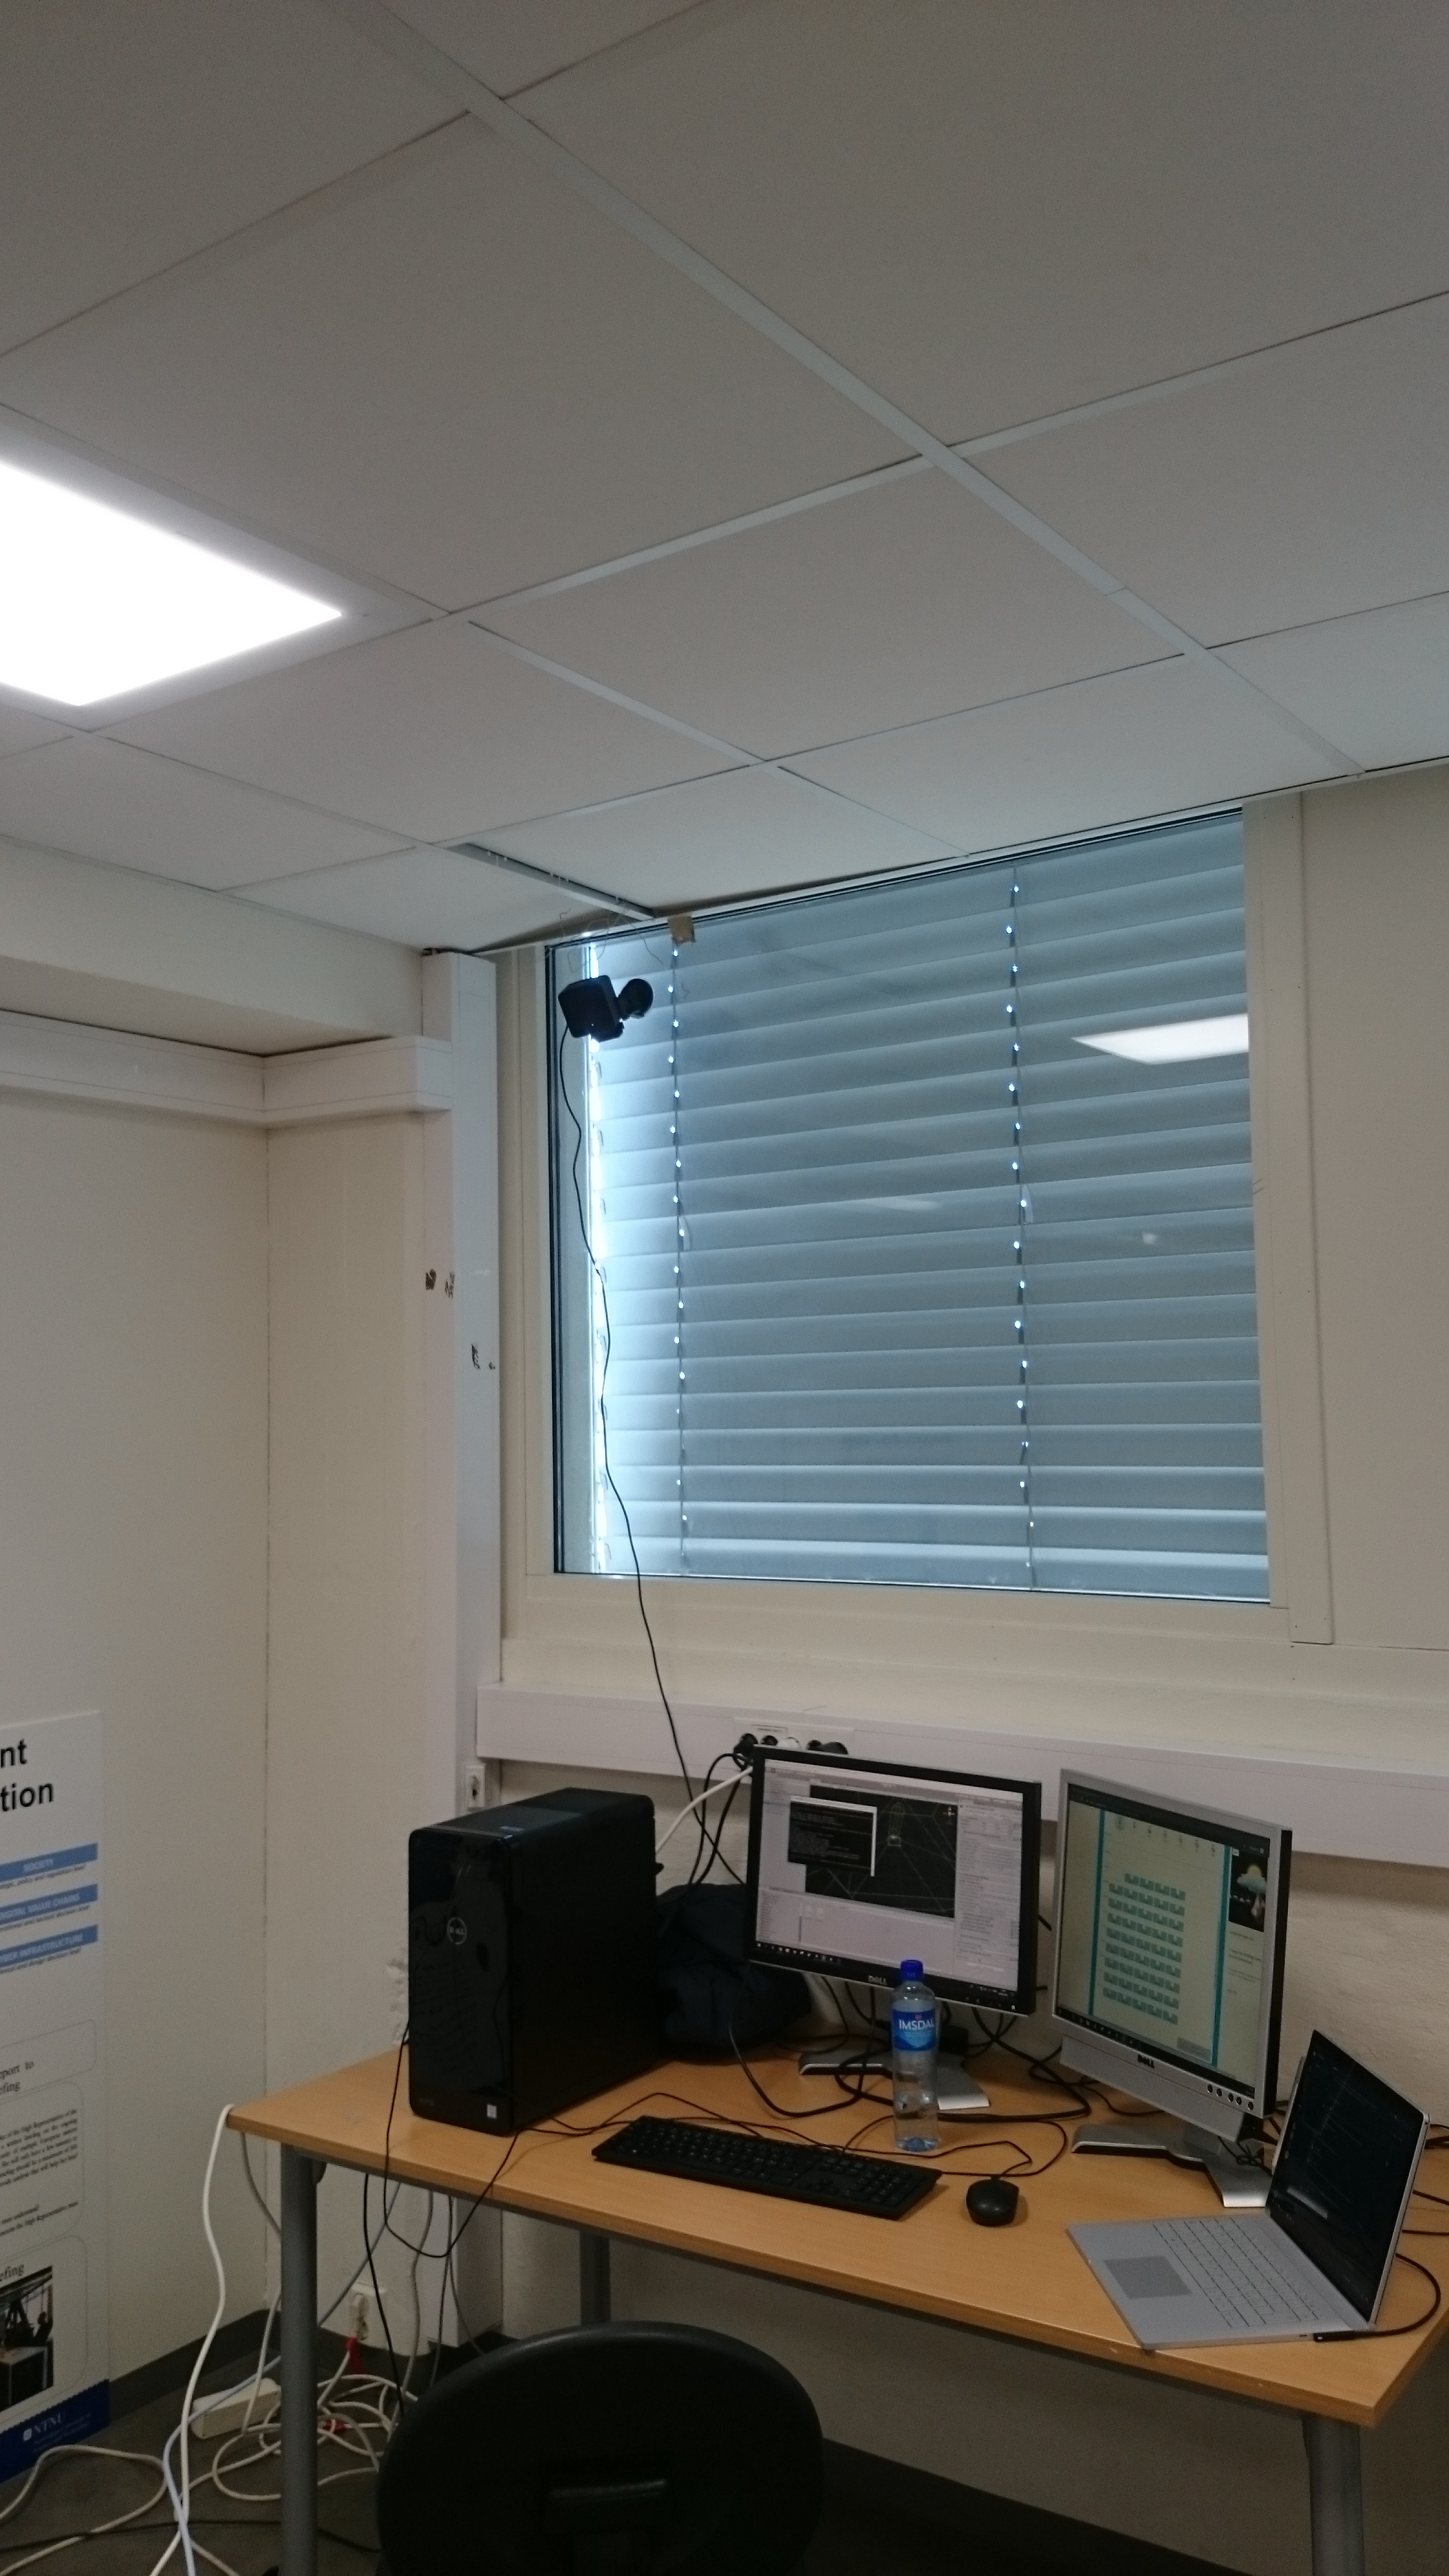
\includegraphics[width=0.25\textwidth]{figures/images/experiment2EnvironmentChanges.jpg}
    \caption[Changes in Experiment Environment for Experiment 2]{This image shows the alternative lighthouse setup that had to be made as the original ceiling mounted lighthouse disappeared before Experiment 2 started. Instead of a ceiling mounted solution, this setup makes use of a glass mounted lighthouse.}
    \label{fig:ex2changedLighthouse}
\end{figure}

There was a 2 week period between Experiment 1 and 2. During this time, one of the ceiling mounted HTC Vive lighthouses disappeared from the experiment setup with no trace or information on where it had gone. As such, it was necessary to setup a new lighthouse in a slightly different configuration. This can be seen in Figure~\ref{fig:ex2changedLighthouse}. The disappearance of the original lighthouse was discovered on the weekend before the experiment started and as such, only limited amounts of room calibration testing was possible. This did create some calibration related problems for two participants. In particular, the reset boundaries became too wide for certain walls and resulted in resets not triggering. These calibration problems were fixed with a software workaround as soon as they were discovered and as such only affected two participants. The number of times the resets failed to trigger for each of these two were also noted down so they could be included with post processing. 

\subsection{Sample}
This section consists of information on how the participant sample was acquired, an overview of the demographics in the sample, what information participants were given and miscellaneous information. 
   
\subsubsection{Sampling Procedure}
The sampling procedure for Experiment 2 was the same as with Experiment 1. It consisted of advertisement by supervisors during lectures, information posters that were  placed around campus, advertisement on the local NTNU Discord\footnote{\url{https://discordapp.com/}} server and general convenience sampling. It should be noted that participants who already took part in Experiment 1 were still allowed to participate in Experiment 2.

A variety of time slots were assigned to a doodle poll~\footnote{\url{https://doodle.com/}} where participants could sign up with an alias for whatever time slot best fit their schedule. Participants were once again compensated with some chocolate for their time, albeit with less than in Experiment 1 since the amount of time spent for this experiment is shorter. In total 15 participants signed up for Experiment 2, albeit only 13 of these showed up. These 13 were randomly distributed between the two conditions using the same Mersenne Twister library~\cite{MersenneTwisterLibraryLink} that previously has been mentioned throughout Chapter~\ref{chap:implementation}. This resulted in 7 participants for the control/S2C only condition and 6 in the experimental/S2C+AC2F condition. 

Acquiring participants for this experiment was generally more challenging as many students mentioned they already were fatigued by constantly taking part in the experients of various master students. As such, a similar sample size to Experiment 1 was not possible to achieve within the same amount of sampling time. 

\subsubsection{Sample Demographics}
The sample itself primarily consisted of students within the age range of 18-24 years. Everyone in the sample were male and only one had to remove any optical corrections while participating. 11/13 participants had previous experience with redirected walking experiments due to a larger overlap from participants who already had taken part in Experiment 1. The general spread of VR experience is not quite as well distributed in this sample as compared to Experiment 1. This can be seen in Figure~\ref{fig:ex2PriorVRExperience} where most participants answered with ''1'' and ''5'' on a Likert scale in terms of their prior VR experience.

\begin{figure}[tbph]
    \centering
    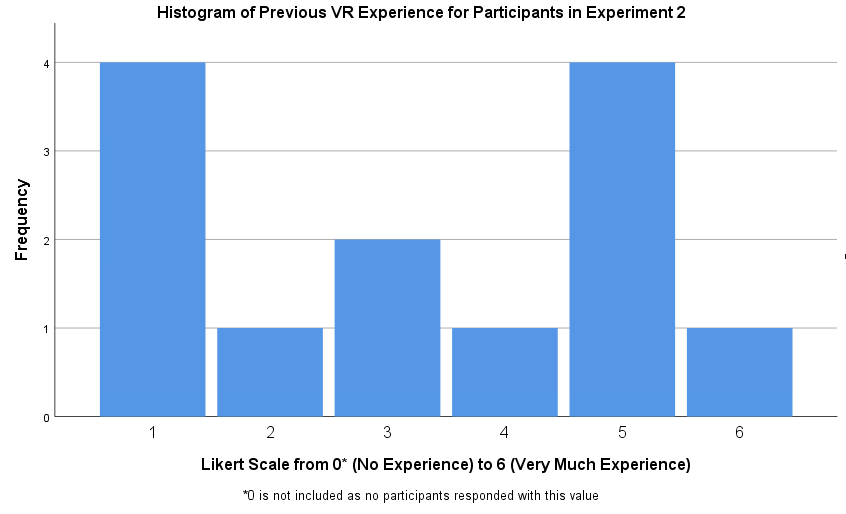
\includegraphics[width=0.75\textwidth]{figures/graphs/PriorVRExperienceExperiment2.png}
    \caption[Histogram on Prior VR Experience of Participants in Experiment 2]{This histogram shows the frequencies of what values participants provided in the demographics questionnaire of experiment 2 in terms of prior VR experience.}
    \label{fig:ex2PriorVRExperience}
\end{figure}

\subsubsection{Information and Consent}
In terms of information and consent, participants were given a sheet that was very similar to the one in Experiment 1. Both information/consent sheets can be seen in Appendix~\ref{app:informationconsent}. Participants were also given some oral information before playing through Ensemble Retriever. This can be summarised as follows:
\begin{itemize}
    \item A very brief summary of what redirected walking is was given if necessary.
    \item If the participant experienced any form of cybersickness at any point they were instructed to mention this so that the experiment could be stopped.
    \item Participants were encouraged to not walk too quickly for their own safety's sake.
    \item Participants were informed that the room tracking might fail for the controllers at times, if so they just need to wiggle it in the air for the problem to resolve.
    \item Participants were told they should be mindful of the tethered cable.
    \item Participants were told that they should not move too much around during battles to avoid potentially moving into walls. 
\end{itemize}

The specific details and wording that was used for this oral information can be found in Section~\ref{sec:ex2information}.

\subsubsection{Miscellaneous Information and Issues}
As mentioned in Section~\ref{sec:ex2environmentchanges}, there were some problems related to the room calibration of the new lighthouse setup that had to be done. This affected participants 1 and 2 in particular where participant 1 experienced one failed reset while participant 2 experienced two failed resets. Failed resets in this case are defined as the reset not triggering when it should. In order to avoid potential skewing of data, the number of times that the resets failed to trigger have been added to these participants during the data post processing step which is mentioned in Section~\ref{sec:ex2postprocessing} and fully detailed in Section~\ref{sec:ex2postprocessingdetails}. 

\subsection{Changes in Ensemble Retriever Between Experiment 1 and 2}
\begin{figure}[tbph]
    \centering
    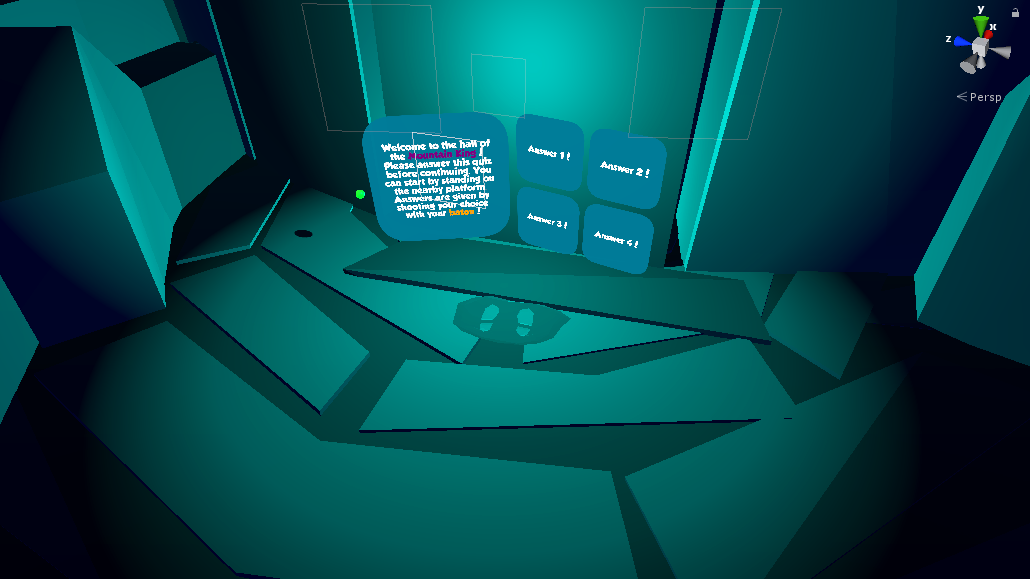
\includegraphics[width=0.5\textwidth]{figures/screenshots/HallOfTheMountainKingWithNewFloor.png}
    \caption[Screenshot of the ''Hall of The Mountain King'' Post Experiment 1]{This screenshot from the Unity scene view shows the updated ''Hall of The Mountain King'' after finishing Experiment 1. Some additional flooring has been added due to participant feedback to make traversal more natural.}
    \label{fig:mkhallWithFloor}
\end{figure}

A variety of things within Ensemble Retriever were changed between Experiment 1 and 2. The full change-log can be found in the project repository~\cite{projectRepository} by looking at the commit history, although this section will provide a summary of the changes that were implemented for Experiment 2. Some of these changes only apply when Experiment 2 is chosen as the active experiment in the software. These changes are marked with ''(EX2)'' while generic changes that apply to the entirety of Ensemble Retriever are marked with ''(ALL)''. The summary of changes are as follows:

\begin{itemize}
    \item Overall walking distance has been reduced to allow for a shorter experiment. (EX2)
    \item The health of the Mountain King has been cut in half to allow for a shorter experiment. (EX2)
    \item The tutorial does not provide any information on detection of redirection as this is only needed for Experiment 1. (EX2)
    \item S2C dampening is re-enabled as it no longer can affect the main focus of data collection. (EX2)
    \item The estimated detection thresholds from Experiment 1 are used as the redirection gains when playing. (EX2)
    \item An extra plane was added to the floor in the ''Hall of The Mountain King''. (ALL)
    \begin{itemize}
        \item This was changed due to feedback as participants mentioned it was awkward to walk between the large holes between the rocks in the floor. The difference can be seen by comparing Figure~\ref{fig:mkhallWithWall} and \ref{fig:mkhallWithFloor}.
    \end{itemize}
    \item The floor in the ''Hall of The Mountain King'' has been better calibrated as the original calibration was lower than it should be, making some participants notice that their height was slightly inconsistent. (ALL)
    \item The buffer between reset and distractor triggers has been increased by 0.5m. This means that resets trigger 0.5m away from physical walls while distractors trigger at 1.5m instead of the previous 1.0m. (ALL)
    \begin{itemize}
        \item The reasoning behind this is that there were observations during Experiment 1 where participants would gradually increase their walking speed as they became more comfortable with the experience. Towards the end, walking speeds were fast enough that there would not be a large enough buffer between distractor and reset triggers, making both trigger instead of only the distractor. By increasing the buffer, the effective size of the walking space is slightly reduced, but should decrease the number of situations where resets trigger right after the distractor itself.  
    \end{itemize}
    \item Distractors like the Contrabass, Oboe and certain phases of the ''Mountain King'' have increased projectile speeds. (ALL)
    \begin{itemize}
        \item This was based on participant feedback for certain projectile attacks taking too long to reach the player, and thus being frustratingly slow. 
    \end{itemize}
    \item The hint providing fireflies in the environment now change colours after the player has visited them. (ALL)
    \begin{itemize}
        \item This was implemented due to participant feedback as a means to make it easier for somewhat disoriented players to see which of the fireflies they already had visited. 
    \end{itemize}
    \item The Distractor trigger magnitude cooldown has been decreased from 1.75m to 1.5m. (ALL)
    \begin{itemize}
        \item This was primarily done due to observations of situations where participants would walk a larger distance right as the death animation of a distractor starts. By the time it was finished and the cooldown initiated, the participant was almost at the bounds of the physical space, resulting in a reset instead of a distractor trigger. 
    \end{itemize}
\end{itemize}
\section{Results}
* Intro

\subsection{Relative Effectiveness}
* Intro
\subsubsection{Legitimate Resets}
* Will focus on legitimate resets. In this case, we want to exclude any resets that mistakenly happen due to the participant not stopping when a distractor has spawned. These would skew the data somewhat so they should preferably be removed. 
* If the participant moves around while fighting and hits a reset this should preferably be avoided as well. 

* Why not just discard all resets that happen when a distractor is active?
    * We want to count resets that may have happened in the period between a distractor defeat and the time it takes for the animation to finish(this is where the transition is fully finished). 
    
    * The minimum time that was spent fighting a distractor was 18.2 seconds.
    * Figure~\ref{fig:minDistractorDefeatTime}
    * As such, a 10 second cutoff point is used to provide some buffer. Any resets happening within the first 10 seconds of a distractor spawning are thus discarded.

\begin{figure}[tbph]
    \centering
    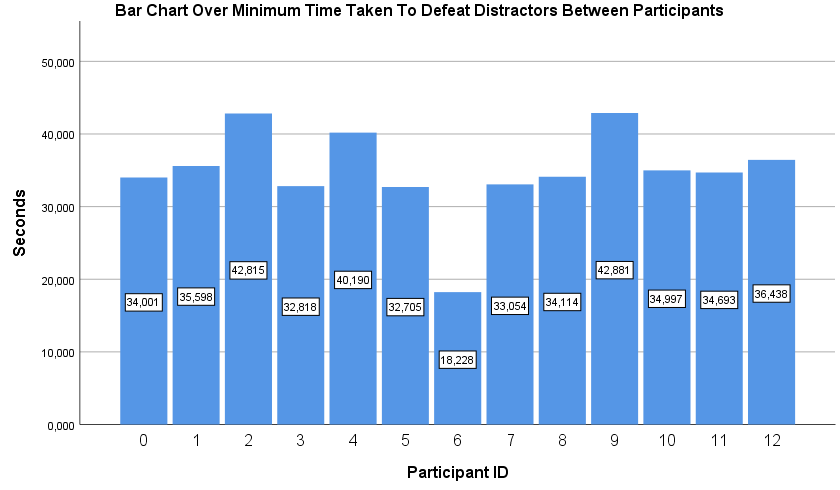
\includegraphics[width=0.75\textwidth]{figures/graphs/MinDistractorDefeatTime.png}
    \caption[Minimum Time Needed To Defeat Distractors Between Participants]{This bar chart shows the minimum time needed for each participant do defeat any distractor in Ensemble Retriever.}
    \label{fig:minDistractorDefeatTime}
\end{figure}

\subsubsection{Time/Walking Speed Normalisation}
* Two variables that potentially could have some effect on the the reset counts between conditions is the time spent on walking and the walking speed of participants. It is thus necessary to first look at the average movement speed and time spent on walking between the conditions. 

* Time Spent Walking is in Figure~\ref{fig:TimeSpentWalkingBetweenConditions}
\begin{figure}[tbph]
    \centering
    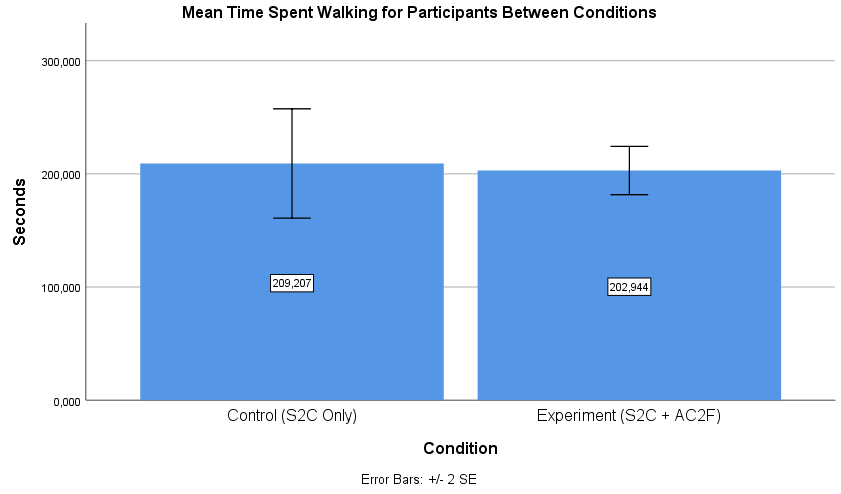
\includegraphics[width=0.75\textwidth]{figures/graphs/TimeSpentWalkingBetweenConditions.png}
    \caption[Mean Time Spent Walking Between Conditions]{This bar chart shows the mean time participants spent on walking between the two conditions.}
    \label{fig:TimeSpentWalkingBetweenConditions}
\end{figure}

* Mean Metres per Second between conditions is in Figure~\ref{fig:ex2mps}
\begin{figure}[tbph]
    \centering
    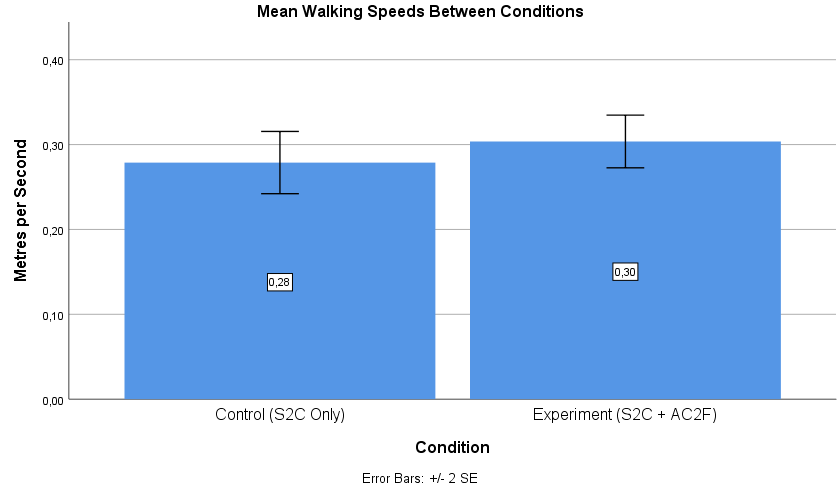
\includegraphics[width=0.75\textwidth]{figures/graphs/mpsBetweenConditions.png}
    \caption[Mean Walking Speed Between Conditions]{This bar chart shows the mean walking speed of participants between conditions.}
    \label{fig:ex2mps}
\end{figure}

* They are pretty similar.\todo{Do I need to do anything more with these two or are they similar enough that I only have to show that they are similar?}

\subsubsection{Mean Number of Resets for Participants Between Conditions}
* Figure~\ref{fig:ex2resetMeans}.
\begin{figure}[tbph]
    \centering
    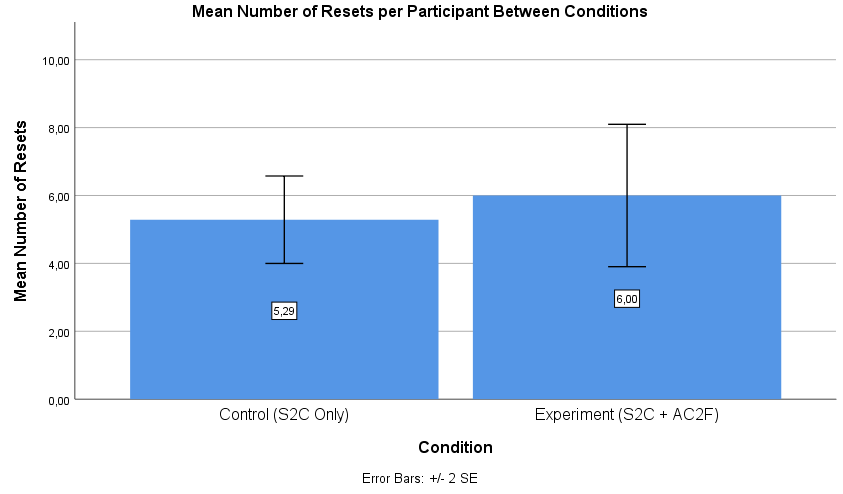
\includegraphics[width=0.75\textwidth]{figures/graphs/ResetMeans.png}
    \caption[Mean Number of Resets Between Conditions]{This bar chart shows the mean number of resets that participants experienced between conditions.}
    \label{fig:ex2resetMeans}
\end{figure}

\subsubsection{Hypothesis Testing}

\subsection{Alignment Time Effectiveness}
\section{Discussion}

* Some initial musings (HALFWAYS THROUGH EX 2): The total number of reorientations may not be significantly different, but the number of times alignments happen and the time needed to align makes AC2F more time efficient and accurate in relation to the goal it wants to reorient you to
* This provides potential benefits in (the next section): 

\subsection{Minimising The Risk of Cybersickness Buildup With Distractors}
* Assuming the results provide some good insight into this:
* If the difference between alignment and interaction time with a distractor is large enough, a possibility would be to decrease the strength of gains as the user will not start to move around again until they have finished interaction. 
* As long as it is possible to align the user by the time they are done, we can decrease the strength of gains and as a result potentially be below the individual thresholds that may trigger cybersickness. 
   * Now this would result in exposure towards rotation gains over a longer period of time than if the gains are strong and align early. Whether strong gains early and no gains aligned or whether continuous weaker gains over a longer time period is optimal is hard to say and would require further study.\todo{Hey, Add me to future work!}
   * Given the possibilities for adaptation effects, the continuous solution might be better as it better adapts the user to the redirected environment. Ultimately it is hard to say though. 
   * While some adaptation style effects were experienced for positive rotation gains in Experiment 1, it is hard to say how much 0 gains during alignment affected the adaptation
 
\subsection{Relationships Between Alignment Fail Rates and Mean Number of Resets}

* One would expect that the higher fail rate of S2C only would have some effects on the rest of the data that was collected in the experiment. Why is it not?
   * Slightly Slower walking speed for S2C Only might be the reason for why those participants on average spent a few extra seconds of walking
   
   * It may be that while the reorientation itself was not entirely complete, it was close enough to avoid the player moving into the reset bounds of any nearby walls. 
   * There may be some effect, but the smaller sample size and low amount of resets that happen per participant makes it hard to actually see this. 
   * At the end of the day, this is just idle speculation. if a user in a corner is reoriented to walk parallel to a wall rather than towards the centre, they will avoid the reset but have a slightly lower amount of time needed until they hit the next distractor or reset assuming they walk straight.
      * It may also be that being reoriented in this manner allows S2C to produce a longer curve for the user to walk on compared to starting towards the centre. This could be one of the reasons for why there is no significant difference in the number of resets \todo{I might be onto something there}
      * When aligned towards the centre, the effective application of curvature gains is essentially halved as it wont be applied again until you pass the centre
      * If you instead point parallel with a wall, you wont lose out on the curvature gain application that you otherwise would if you were aligned with the centre
      
      * While the fail rate is higher, it may mean that it manages this more optimal curve more frequently than S2C+AC2F, but it also manages more unoptimal curves, resulting in a similar mean due to inconsistency
      * It would be interesting to compare the actual paths that participants travelled to look deeper into this.
         * RDW toolkit technically has visualisations for this implemented, but not the actual data storage of the path. Implementing a solution for this would allow for this thing to be tested
      * If the user on the other hand is roughly on the middle of one wall, then being redirected towards the centre would most likely be better.
      * As such, it may be that we should dynamically create the alignment goal heuristics depending on where the actual distractor or reset happens. 
\chapter{General Discussion}\label{chap:discussion}
This chapter consists of a more general discussion that is not directly tied to either of the two experiments. 

\section{Limitations of the Current AC2F Heuristic}
While the AC2F algorithm has worked relatively well for Ensemble Retriever, it is worth considering the walking scenario that the algorithm has been used for. For Ensemble Retriever, the explorable space is large and open. This results in reasonably straight paths between fireflies until the player reaches the final portal. Furthermore, the player does not stop at any point and move in the opposite direction, which is favourable for the sampled future path heuristic. If the player on the other hand reaches a point and then decide to do a 180-degree virtual turn, the employed heuristic may not be as effective if they recently interacted with a distractor. In this case, a new distractor would need to be triggered, or a reset would occur. 

On the flip side, AC2F as an algorithm does not need to use a sampled future path heuristic. Any sort of directional heuristic could be used. As such, in more confined spaces, it could be possible to use more predictive heuristics for AC2F instead of a sampled future path. In general, if there are situations where the developer knows the direction a user will take, it may be more effective to have some set heuristics which can be used. As far as a generic solution is concerned though, creating a heuristic out of sampled position changes is relatively simple and works well for open areas. 
   
\section{Salience and Distraction}
One element which is worth some further discussion is the pre-existing salience in the virtual environment. As priorly mentioned in Chapter~\ref{chap:relatedWork}, current research has suggested that a larger distribution of salient elements in a scene decreases the effectiveness and focus on other salient objects~\cite{sitzmann2018saliency}. In general, the various salient elements in Ensemble Retriever could be summarised as such:

\begin{itemize}
    \item Environmental glowing mushrooms which always are visible.
    \item Hint providing fireflies which only are visible outside of battles.
    \item The portal that sends the player to the Hall of The Mountain King. 
    \item Any distractors that the player battles.
    \item The projectiles that a distractor fires at the player. 
\end{itemize}

The salience provided by the mushrooms and portal could for example interfere with the salience that a distractor provides by itself and together with its projectiles. Some participants have also mentioned that they used the mushrooms as a reference point to detect redirection as it made detection easier. This could be a result of the salient mushrooms providing a more considerable degree of optical flow in an otherwise darker environment. This would also correspond somewhat with the speculation for as to why it was somewhat easier to notice negative rotation gains during battles as the distractors would create additional optical flow as well. One option to mitigate this would be to decrease the overall salience in the scene. Despite this, if we think practically and realistically, a darker scene or environment will usually consist of a certain amount of salient regions for the sake of illumination. As such, this should likely be kept in mind when working with such scenes. In any case, it would be interesting to see further research into how salience could affect optical flow and how this further could affect the noticeability of redirection.

\section{The Ideal Timing for Switching Redirection Algorithms}\label{sec:idealAlgorithmTimingSwitch}
Throughout both experiments, one observation of note was when participants started to move again after finishing a distractor battle. Most participants waited until the fireflies became visible again, meaning that the transition from AC2F to S2C was finished. Some participants on the other hand started to move as a distractor was still playing through its death animation. In the current solution, the switch from AC2F to S2C happens when this animation is finished. This means that if the player starts to move as this animation is playing, they will not be exposed to any curvature gains for a little while. Rotation gains would not be applied either if AC2F finished alignment. This means that the effective redirection is decreased for a small space of time. 

Another problem with starting to walk this early is that distractors have a distance cooldown that needs to be travelled before they can be spawned again. This cooldown only starts to tick down from movement after the switch from AC2F to S2C is finished. As a result, starting to move early might result in hitting a reset instead of a distractor as it still is on cooldown. This can happen as the cooldown did not track how much the player moved before the algorithm switch. One option to deal with this would be to switch algorithms as soon as a distractor's health reaches zero, but this also has a downside. If AC2F did not finish alignment, then this small remaining time could be used to apply further redirection and potentially complete alignment. 

In general, a better solution could be to choose this timing in a more dynamic fashion. For example, if the future path already has been aligned, then the switch from AC2F to S2C could trigger instantly when a distractor's health reaches zero. If alignment has not happened on the other hand, the switch could be delayed like it currently is to have some additional time for finishing alignment. As far as the distance cooldown for distractors is concerned, it is likely best to start counting this one as soon as it is detected that the player has started to move again. This could be triggered by using a movement threshold to check whether the player has started to move or not.  

If AC2F as an algorithm were to support curvature gains in the future, then this would not require any changes to the timing of algorithm switches. At that point though, it might not be necessary to use S2C as an algorithm as AC2F could take care of everything. If AC2F supported curvature gains, then it likely would have been closer to the mentioned ''modified S2C'' that Peck et al. + Chen and Fuchs have mentioned in their work~\cite{peck2010improved, chen2017towards, chen2017supporting}. This would of course increase the complexity of the algorithm by a little bit, which is why this was not implemented in this thesis as it was outside of the allocated resource budget.

\section{Effectiveness of Integration From a Game Design Point of View}
While Ensemble Retriever's fully integrated distractors have been reasonably effective in terms of reorienting players away from physical walls, it is also worth to look at the integration from a game design point of view. 

In general, participants did seem to enjoy the experience. Some excerpts from when participants were asked whether they enjoyed their experience includes:

\begin{itemize}
    \item ''Yes, it was very fun to play! I enjoyed the gameplay as it was quite original.''
    \item ''Yes, very enjoyable.''
    \item ''Quite fun, would be interesting to see multiple enemies at a time.''
\end{itemize}

General feedback mentioned that the enemies in Experiment 1 were a bit slow. This was addressed in Experiment 2 by increasing the speed of attacks for relevant distractors and was positively received by the participants that took part in both experiments. 

Despite this, it was noticeable that participants got somewhat tired of facing the same distractors again and again towards the end of the experience. The frequency of distractors relative to the length of time spent on fighting them could also be a factor in this. This could be mitigated by having a more extensive variety of distractors that players can fight instead of just five varieties. Furthermore, introducing other types of distractors which are different from the battle ones could also decrease the monotony towards the end. 

A more immediate solution that would not cost as many resources though would be to decrease the time spent on fighting distractors as mentioned in Section~\ref{sec:ex2MinimisingCybersickness}. While the distractor battles likely are the most engaging part of the experience, the time taken to reach the portal is relatively long. This is of course a limitation with having to perform experiment measurements, and in a real-world scenario the current implementation could have worked better if the overall walking distance was shorter. 

From a game design point of view, a shorter experience would likely work better and in particular if the player does not have both their shield and baton at the maximum level by the end. This would emphasise player choice as players would need to choose their upgrades more carefully since they would not have all of them when fighting the Mountain King. This would allow players to either specialise in offence or defence depending on their personal preferences. While the current implementation allows the player to choose between upgrades when levelling up, the choices do not matter much as they will have a high enough level to unlock all the upgrades later on. Another option to further emphasise player choice would be to allow one final specialisation upgrade for either the shield or baton. The specialisation could in this case only be allowed to choose once regardless of how high the player's level is. This way, the player would need to choose which of their tools receives the final upgrade.  

\section{Practical Challenges for Distractors in Redirected Walking}
There has been a variety of practical challenges with distractors that have been observed while conducting Experiment 1 and 2. This section discusses these and provides some potential solutions. 

\subsection{Movement During Battles}
While most participants stood relatively still while fighting distractors, some also moved around quite a bit. This movement creates some challenges as distractor battles always will be roughly 1m away from any reset bounds and 1.5m away from physical walls. If a participant moves around a lot, they might end up hitting a reset boundary which would be somewhat distracting to deal with in the heat of battle. While distractors and projectiles are paused during resets, it could still be considered as unwanted behaviour. The question then becomes: how do we limit the movement of certain players while they battle distractors? One potential option could be to make better use of deterrents to avoid having any players move further than 1m away from where their battle started. For example, certain objects could be strategically placed like the fire walls in Chen and Fuchs' research~\cite{chen2017towards, chen2017supporting} to deter the player from moving further. This was ultimately out of scope for the development of Ensemble Retriever, but could be considered as a potentially useful solution.  

\subsection{Stopping Speeds}
Another practical challenge is the buffer between reset and distractor trigger boundaries with respect towards walking and stopping speeds. Ideally, the player should have as much walkable space as possible without triggering a distractor and then an immediate reset. While a 1m buffer between the two bounds has worked relatively well in Experiment 2, there were still some cases where the buffer was too small. In a similar fashion to dealing with movement during battles, it might be possible to further increase the stopping speed of participants with effective use of deterrents. As an example: the contrabass distractor spawns and immediately boxes the player into some sort of battle arena. The player might then end up stopping a bit faster compared to the current situation where the distractor simply spawns a few metres in front of them. While it is not guaranteed that this would solve the problem, it should at least be expected that players stop slightly faster to avoid crashing into a close virtual obstacle.

\subsection{Concrete Distractors in Confined Spaces}
Finally, one apparent problem with concrete distractors that make use of much movement is their use in more narrow or confined spaces. In Ensemble Retriever, this becomes an issue when fighting a distractor while close to the portal. In this case, there are potential situations where the distractor might end up moving into or behind the scenery as it rotates around the player. This behaviour is of course not wanted as it obscures vision towards the enemy and makes it harder to play. The question then becomes: how do we deal with distractors when the space around the player is more confined or narrow?

This could potentially be solved by analysing and letting the distractors know when they are in a more narrow area. With this additional knowledge, the distractor could for example move slightly closer to the player or limit their movement abilities to better work with their current environment. Finding a generic solution in this case is probably hard given the context-sensitive nature of fully integrated distractors. While generic solutions may be challenging to create for this, there are context-specific optimisations and solutions that can be developed. Outside of slightly more dynamic movement behaviour, it could be possible to have a set of distractors which specifically are aimed to work in more narrow spaces. If the game then detects that the player needs a distractor and is in a narrow space, it can spawn from this alternative distractor list to better suit the specific area. This way, it could also be possible to optimise how much the player moves their head around despite the limitations of the narrower space around them. 
            
\section{Participant Feedback on Pause - Turn - Centre}
While it was not directly measured or focused on, some participants gave oral feedback on the Pause - Turn - Centre resetter. The general feedback was positive in that it felt natural and easy to use whenever needed, although it took some time to get used to the resetter initially. Participants who moved a lot during battles managed to trigger a few resets while fighting. They mentioned that it was rather disruptive and disorienting when it happened, which is to be expected. As far as the various goals of Pause - Turn - Centre are concerned, it managed to safely reorient participants away from physical walls and did not result in any issues in terms of HMD cable wrapping. As far as participant feedback is concerned, none mentioned the reset as causing cybersickness. This is of course anecdotal though and would require a separate experiment to properly measure. In general though, no negative feedback was given in relation to Pause - Turn - Centre. 
\chapter{Conclusion}\label{chap:conclusion}
* Summary
* This was a pretty exploratory study into relatively unexplored waters
   * Resulted in a lot of future work!

What were the findings on different levels?
   * What has the research provided insights on in
      * The specific distractor/redirection level
      * Redirected walking as a whole
      * General impact in VR
      * ETC


\section{Future Work}\label{sec:futurework}
Where would the project go from here. While this section focuses on areas of future research that were detected through discussion and results, it may not guarantee that there are not already existing papers or research already looking into this. The literature sample for this thesis is not comprehensive enough to cover the entirety of the redirected walking space, but serves as an approximation in relation to the main topic of distractors within redirected walking. 

* What can be improved
* AC2F
   * Could become more generic by adding support for walking around
   * Smoothing can be improved
   * Potential studies into the effect of smoothing solutions on detection thresholds

* Looking deeper into the asymmetry between positive and negative rotation gains. 

* Identifying the variables that affect why there is a significant difference that widens the detection thresholds when walking. (The data variability most likely has a pretty strong effect on why it is like it is for negative rot gains)
   * Is expectation mismatch relevant when fighting as you do not have quite a set target to look at when walking?
      * Goal directed looking
   * Frame of reference
      * Can the moving distractor be considered a frame of reference for redirection?
      * This is of course anecdotal, but some participants mentioned using the glowing mushrooms as a frame of reference, but S2C still goes lower than AC2F on average on negative gains
      * Optical flow/visual density generated by distractors
         * Since some participants mentioned they used the glowing mushroom as a reference point to notice redirection, would a distractor work as one of these reference points?
   * Differences in algorithms
      * Smoothing solution for AC2F may be an effect
      * If alignment as a concept is disabled from AC2F you will be able to apply more rotation gains to the participants during battles
         * This would help with the asymmetry in number of detections between algorithms, more time would likely be spent with AC2F than S2C in terms of potential space to detect gains
         * Might also result in stronger adaptation effects
            * We would need further studies into how temporarily disabling gains affects adaptation effects

* Improving data recording
   * improving accuracy of variables, automating data post processing by handling this on the software side. 

* Other interesting pathways
   * Having people's first experience with VR be with redirected walking
      * They might normalise the redirected walking elements
         * \todo{Will have to look deeper into the data on people with no experience and how many detections they did}
   * Effectiveness of disabling redirected walking towards the end of an experience to help the user get accustomed to normal head rotation before taking off the HMD
   
   * Looking deeper into why reorientations using S2C may be better off doing a reorientation that is parallel to walls at times rather than towards the room centre
      * Could be simulated with the toolkit for example to see whether relative effectiveness increases compared to 
      
   * What is optimal in terms of cybersickness when using distractors? Stronger gains for short periods of time with no redirection breaks when aligned or lower gains throughout the entire distractor usage
   
   * How does temporarily disabling gains affect adaptation effects?
   
   * Looking deeper into how prior VR experience affects noticability. 
   
   * effective and short Individual DT calibration methods

\ifthenelse{\boolean{HarvardCitations}}{%
	\bibliographystyle{agsm} % used for Harvard style references. Names - Humanities & Interaction Design
}{%
	\bibliographystyle{ntnuthesis/ntnuthesis} %used for Vancover style references. Numbers - Computer Science & Physics
}

\bibliography{MastersExample}

\appendix
\chapter{Terminology and Abbreviations}\label{app:terminology}

\begin{description}
\item[VR -] Virtual Reality.
\item[VE -] Virtual Environment.
\item[ROT -] Reorientation Technique. These are used in redirected walking whenever the user is close to leaving the physical tracking space in order to reorient them away from it. 
\item[NPC -] Non-playable character. A term used in video games to classify a computer-controlled entity.
\item[HUD -] Heads-Up Display.
\item[GUI -] Graphical User Interface.
\item[S2C -] ''Steer To Center''. A redirection algorithm that applies gains in a manner that redirects the user towards the centre of the tracking space.
\item[S2O -] ''Steer To Orbit''. A redirection algorithm that applies gains in a manner that redirects the user to walk on the edge of a circle in the tracking space.
\item[FoV -] Field of View.
\item[HMD -] Head Mounted Display. Also often known as a virtual reality headset.
\item[IDE -] Integrated Development Environment.
\item[2AFC - ] Two-alternative Forced Choice.
\item[AC2F - ] ''Align Centre To Future''. A redirected walking algorithm that has been developed for this thesis. Focuses on redirecting a standing user so their future walking direction is aligned with the centre of the physical space.
\end{description}
\chapter{Reproducing The Experiments} \label{app:reproduction}
* All the necessary steps needed to reproduce the experiment

\section{Before Starting}
* Room setup
* Software Setup
* Hardware Setup

\section{Experiment 1}
* What do you have to do to run it?
* What information were participants given?

\subsection{Participant Information}\label{sec:ex1information}

\subsection{Data Recording/Data Format}\label{sec:ex1dataformat}
* Data is recorded as a series of frames.

\begin{description}
   \item[ParticipantID: ] The unique identifier for the current participant. Integer format, increments per participant. 
   \item[GainDetected: ] Whether a gain was detected this frame
   \item[DeltaPosMagnitude: ] The strength of movement that the participant has moved between frames
   \item[DeltaDir: ] The angle that the participant's head has rotated on the vertical axis between frames
   \item[DeltaTime: ] The time between frames in seconds
\end{description}
* After this a variety of columns are dedicated whether specific elements have been active or not this frame. The values are 1 if true or 0 if false.
* These binary columns stop after the CurvatureGainApplied column. 

* Then:
\begin{description}
   \item[CurrentRotationGainAgainst: ] Current negative rotation gain. Read as a percentage
   \item[CurrentRotationGainWith: ] Current positive rotation gain. Read as a percentage
   \item[CurrentCurvatureRadius: ] Current curvature radius. Read in metres. 
\end{description}

* Then ratios. These only contain data when GainDetected == 1. The various ratio columns make up the ratio of gains that were applied in the last half second once the detection button was pressed

* Remaining columns:
\begin{description}
   \item[MostLikelyDetectedGain: ] The value of the gain that had the largest ratio at the time of detection. Can be 0 in a few cases which are further discussed in Section~\ref{sec:ex1postprocessing}
   \item[TimeSinceExperimentStart: ] The time in seconds since the participant finished the tutorial and started playing
   \item[AlgorithmCategory: ] Categorical variable for the currently active algorithm. 0 for S2C and 1 for AC2F.
   \item[AppliedGainCategory: ] Categorical variable for the currently applied gain. -1 for none, 0 for neg rot, 1 for pos rot, 2 for curvature gain
   \item[DistractorCategory: ] Categorical variable for what current distractor is active. (0 = None, 1 = Contrabass, 2 = Oboe, 3 = Harpsichord, 4 = Violin, 5 = Glockenspiel)
   \item[MostLikelyDetectedGainCategory: ] Categorical variable for the type of gain that most likely was detected. Same labels as AppliedGainCategory.
\end{description}

\todo{Could extract one line from the data and use it as an example}

\subsection{Data Post Processing}\label{sec:ex1postprocessingdetails}
* While SPSS was used for processing, this section will primarily focus on the thought process behind the detections to be more applicable for other statistics software as well. 

* Section~\ref{sec:ex1postprocessing} in methods mentions four potential cases for when the MostLikelyDetectedGain value is at 0. This section will go through how to process steps 1 and 4 into proper detection values. 

* This post processing step is primarily used for rotation gain detections as these are a bit more complex to deal with than curvature detections as they can vary between their original value and 0 in cases like being aligned under AC2F. 

* MostLikelyDetectedGain can either be updated through these two post processing steps or it could be handled in a copy of the variable (recommended for the sake of keeping history)

\subsubsection{Extracting Additional Rotation Gain Detections for Case 1}
  * Case summary: The user detected a rotation gain, but by the time they pressed the button, AC2F had already aligned them and rotation gains were disabled.

  * First: CurrentRotationGainAgainst and With are both set to 0 whenever the user has been aligned. This can be a bit problematic for post processing so the first step is to create a copy of these variables that simply repeat the last value of the gains before alignment zeroes happen. This will make it easier to extract rotation gains down the line. 

  * There are two different approaches that can be used to extract rotation gains with a value of 0 in case 1. The first is simpler, but less effective while the second is a bit more complex, but should provide more additional detections. 

  * Alternative 1: Using the MostLikelyDetectedGainCategory variable:
     * Selection: Gain Detected = 1 AND MostLikelyDetectedGain = 0 AND CurrentRotationGainAgainst = 0 AND MostLikelyDetectedGainCategory != -1
     * CurrentRotationGainAgainst and With will both be 0 in this case. It does not matter which one is used for selection. 
     * MostLikelyDetectedGainCategory can then be used to figure out which gain was applied. The value of it will be the gain type that had the largest ratio within the 0.5 second buffer. By using this variable, we can then set the value of the extracted gain to that of the relevant gain from the first step. 
     * This is the simplest approach, but may not provide as many additional detections as the next one. 
     
  * Alternative 2: Using the included ratios (a bit more of a detailed approach)
     * Selection: Gain Detected = 1 AND MostLikelyDetectedGain = 0 AND CurrentRotationGainAgainst = 0 AND NoGainRatioDuringDetection != 1
     * This will provide cases where the majority of the ratio says no gains were applied, but the 2nd largest ratio can be used to determine the correct gain. 
     * We can then check which of the two ratios for rotation gains were largest and use this highest one to determine which rotation gain actually was detected

\subsubsection{Extracting Additional Rotation Gain Detections for Case 4}
  * Case summary: The user detected a rotation gain, but pressed the button slightly late after finishing a head rotation so the 0.5 second buffer primarily points towards that no gains were applied. 

  * This will need to be handled in a similar way to working with ratios from dealing with case 1
  * Selection: Gain Detected = 1 AND MostLikelyDetectedGain = 0 AND CurrentRotationGainAgainst != 0 AND NoGainRatioDuringDetection != 1
  * In this case, gains are still active so we want to make sure that CurrentRotationGainAgainst or With reflect this. It does not matter which one is used. 
  * Similar to alternative 2 from case 1, we can then extract a rotation gain value depending on which of the two that had the largest ratio.

\section{Experiment 2}
* What do you have to do to run it?
* What information were participants given?

\subsection{Participant Information}\label{sec:ex2information}

\subsection{Data Recording/Data Format}\label{sec:ex2dataformat}

  * What is recorded?
  * How can it be understood?

\begin{description}
   \item[ParticipantID:] Unique ID for the participant.
   \item[GroupID:] The ID of the condition that the participant was placed in. (0 = S2C Only/Control Group, 1 = S2C+AC2F/Experiment Group).
   \item[TimeSinceExperimentStart:] The time in seconds since the participant finished the tutorial and started playing. Accumulates over time. 
   \item[TimeSpentWalking:] The time in seconds that the participant has spent walking. Accumulates over time while no distractors are active. 
   \item[NumberOfResets:] The number of resets that have happened so far. It is incremented on the frame that a reset has been triggered. 
   \item[NumberOfDistractors:] The number of distractors that have been triggered so far. Works in a similar fashion to NumberOfResets.
   \item[IsResetActive:] A binary value that either is 0 if no reset was active on a given frame or a series of 1's for as long as a reset has been active. 
   \item[IsDistractorActive:] Similar to IsResetActive, but for distractors instead.
   \item[CurrentlyActiveDistractorType:] Categorical variable for what current distractor is active. (0 = None, 1 = Contrabass, 2 = Oboe, 3 = Harpsichord, 4 = Violin, 5 = Glockenspiel)
   \item[AlignmentComplete:] Binary variable that is set to 1 whenever the user's future path has been aligned with the centre of the physical space. Value is reset back to 0 after the distractor that resulted in the alignment has been defeated. 
   \item[AlignedThisFrame:] Set to 1 on the frame that alignment to the centre of the room has happened. This makes it easy to find all the times where the user has been aligned and gather additional information.
   \item[TimeTakenUntilAlignment:] The time in seconds needed for a distractor to align the user's future path to the physical room centre. This variable only consists of a proper value when AlignedThisFrame is 1 and is 0 otherwise. 
   \item[DistractorDefeatedThisFrame:] Similar to AlignedThisFrame, but is set to 1 on the frame that a distractor has been defeated instead. 
   \item[TimeTakenToDefeatDistractor:] Consists of the time in seconds needed to defeat the currently active distractor. This variable only has a value other than 0 when DistractorDefeatedThisFrame is 1. 
   \item[CurrentPlayerShieldLevel:] The current level of the player's shield. 
   \item[CurrentPlayerBatonLevel:] The current level of the player's baton. 
   \item[DeltaPos:] The strength of movement that the participant has moved between frames. To be more specific it is the magnitude of DeltaPos. 
   \item[DeltaDir:] The angle that the participant's head has rotated on the vertical axis between frames.
   \item[DeltaTime:] The time between frames in seconds.
\end{description}


\subsection{Data Post Processing}\label{sec:ex2postprocessingdetails}
  * Discarding resets that happen due to participants moving too much around while fighting
  * LAG Function to detect reset activation patterns
 
 * TimeSinceExperimentStart will uniquely always be 0 one time per participant. It can be used to filter out cases where one might want to grab one row per participant

* Finding and adding penalties
\chapter{Demographics Questionnaire}\label{app:demographicsQuestionnaire}
This appendix includes the demographic questionnaire which was used for Experiment 1 and 2 in this thesis. 

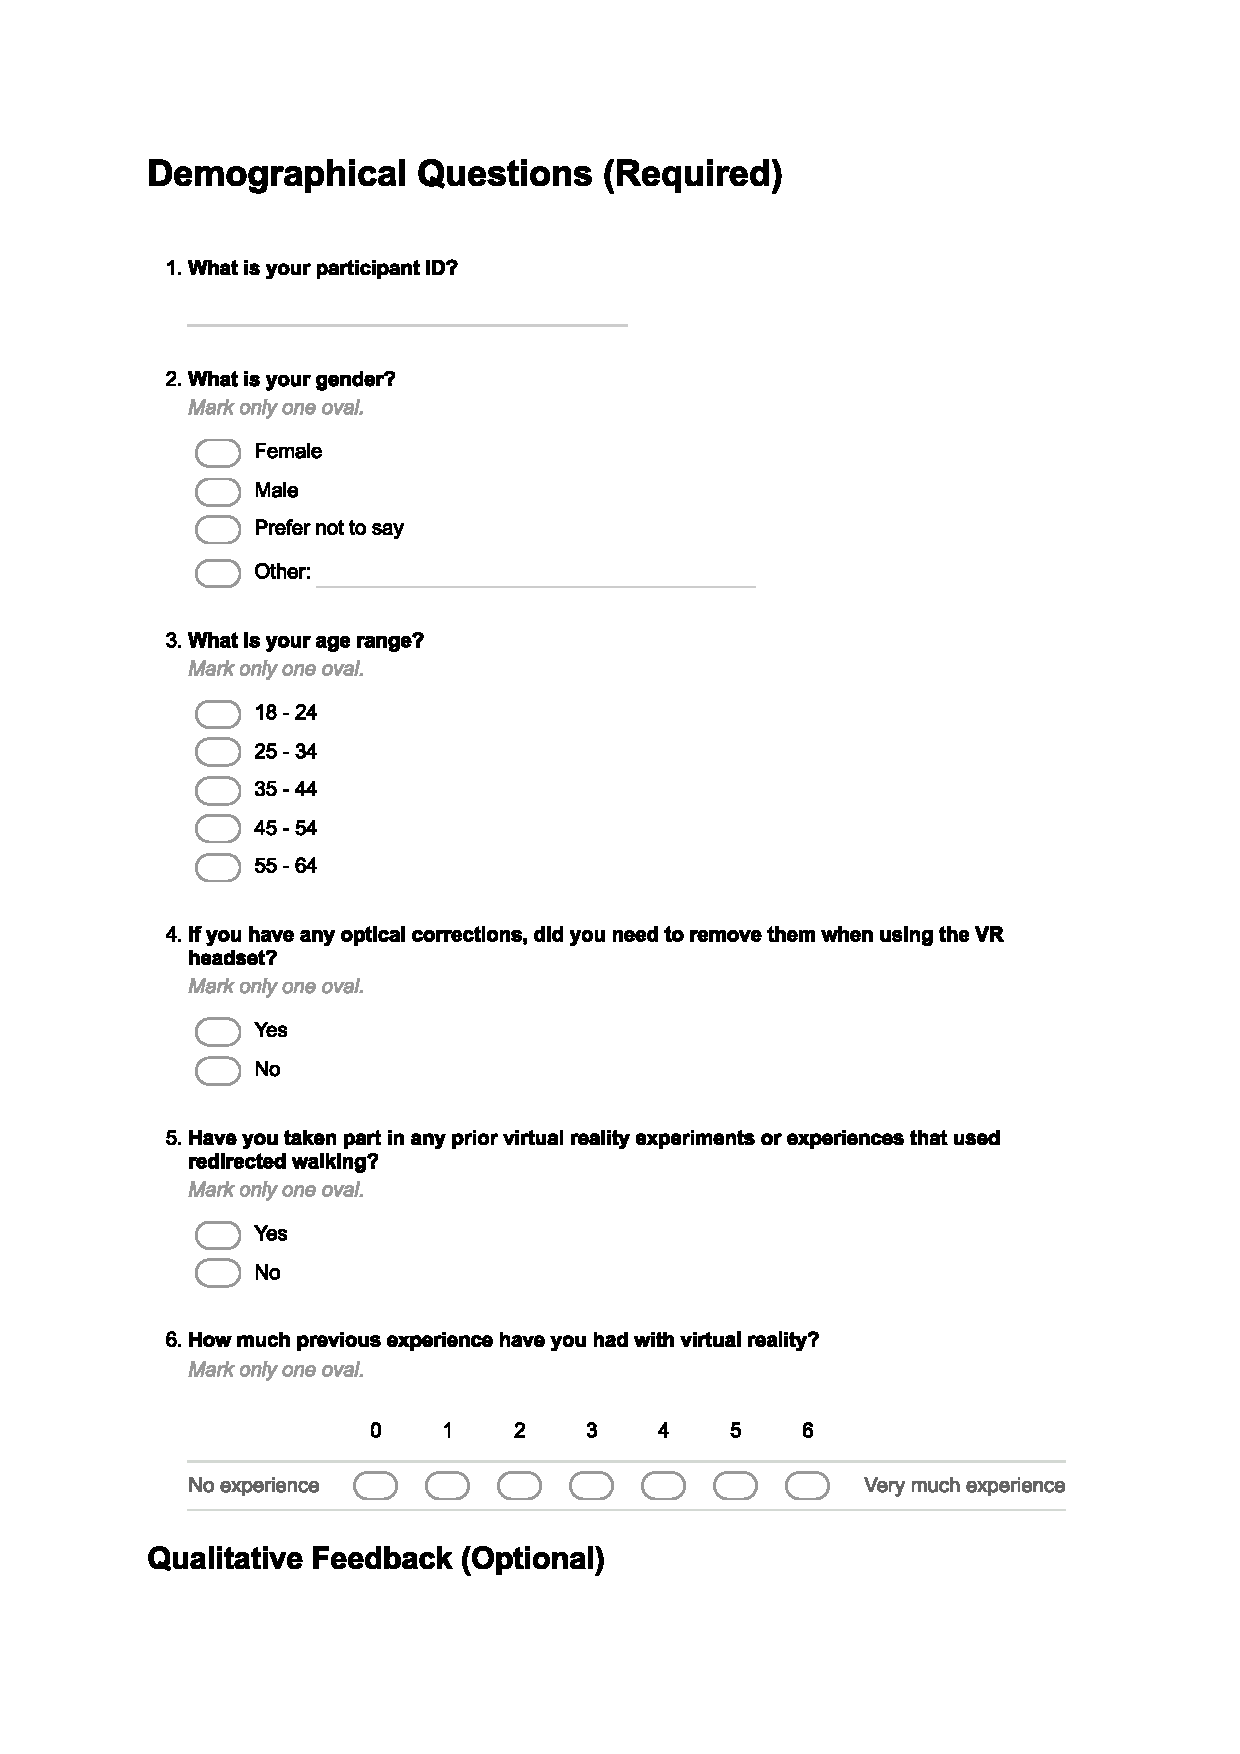
\includepdf[pages=-,pagecommand={},width=\textwidth]{pdfs/surveyExperiments1_2.pdf}
\chapter{Information Sheets}\label{app:informationconsent}
This appendix includes the information and consent sheets that were given to participants throughout experiments 1 and 2. The sheets are mostly the same with some minor differences in terms of mentioned experiment duration and similar smaller details.  

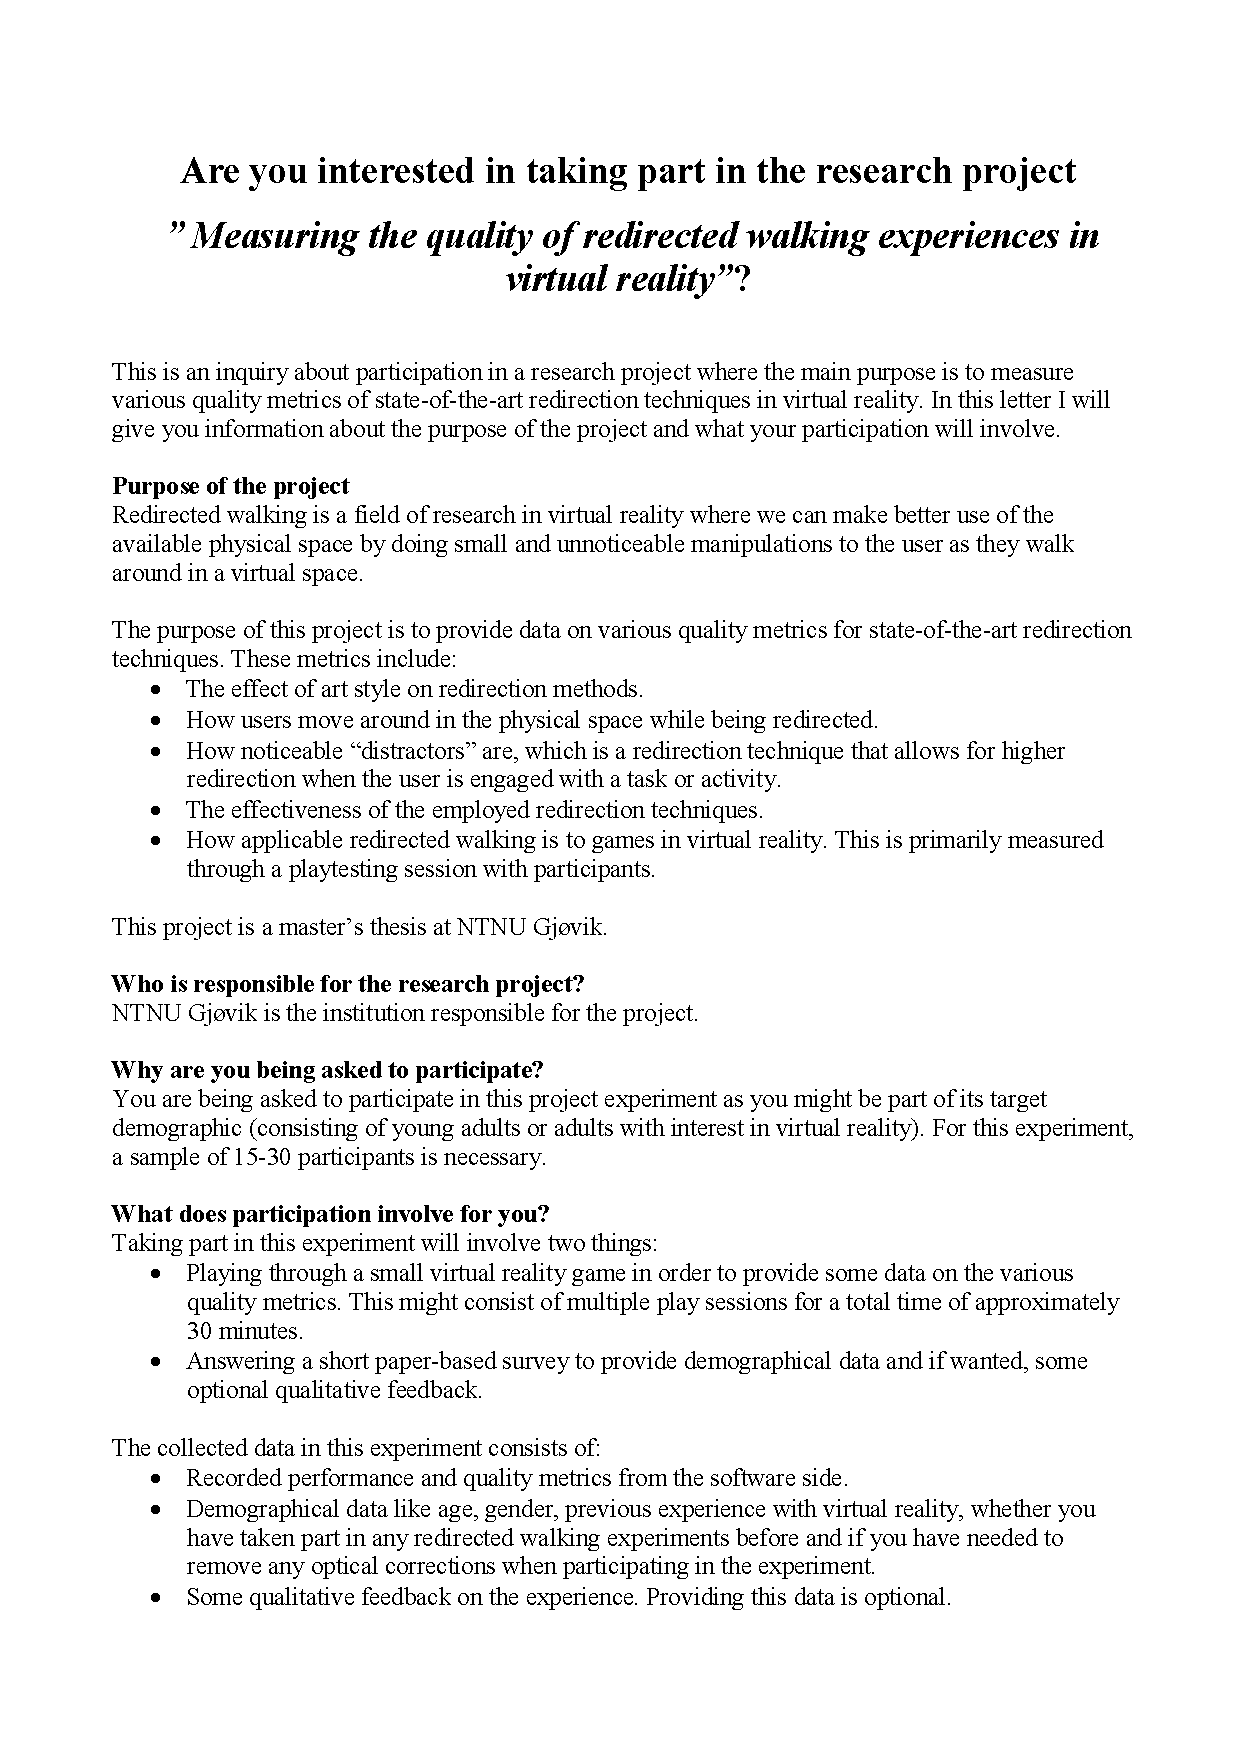
\includepdf[pages=-,pagecommand={},width=\textwidth]{pdfs/informationLetterExperiment1.pdf}
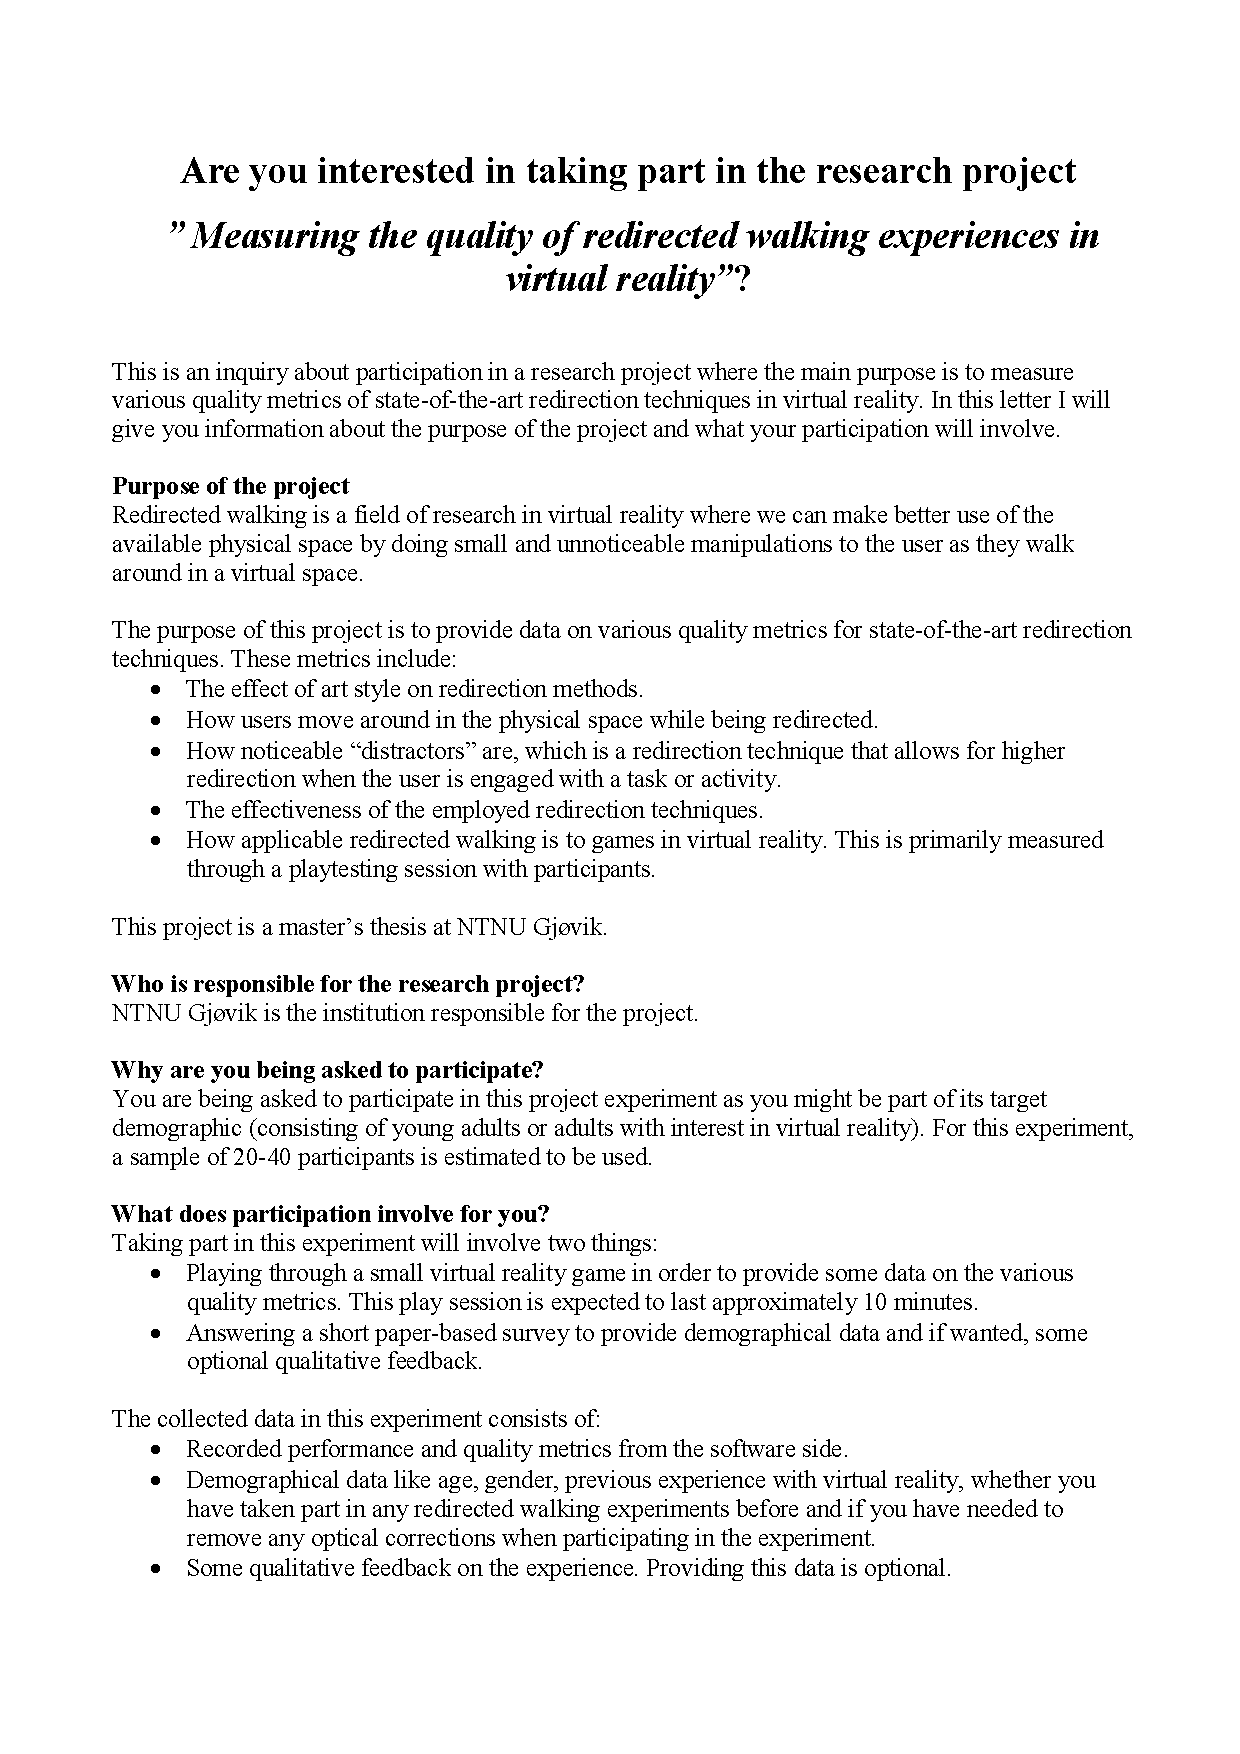
\includepdf[pages=-,pagecommand={},width=\textwidth]{pdfs/informationLetterExperiment2.pdf}
\chapter{Approval - NSD}\label{app:nsdApproval}
The following two pages consist of a copy of NSD's approval for the data collection in this thesis.

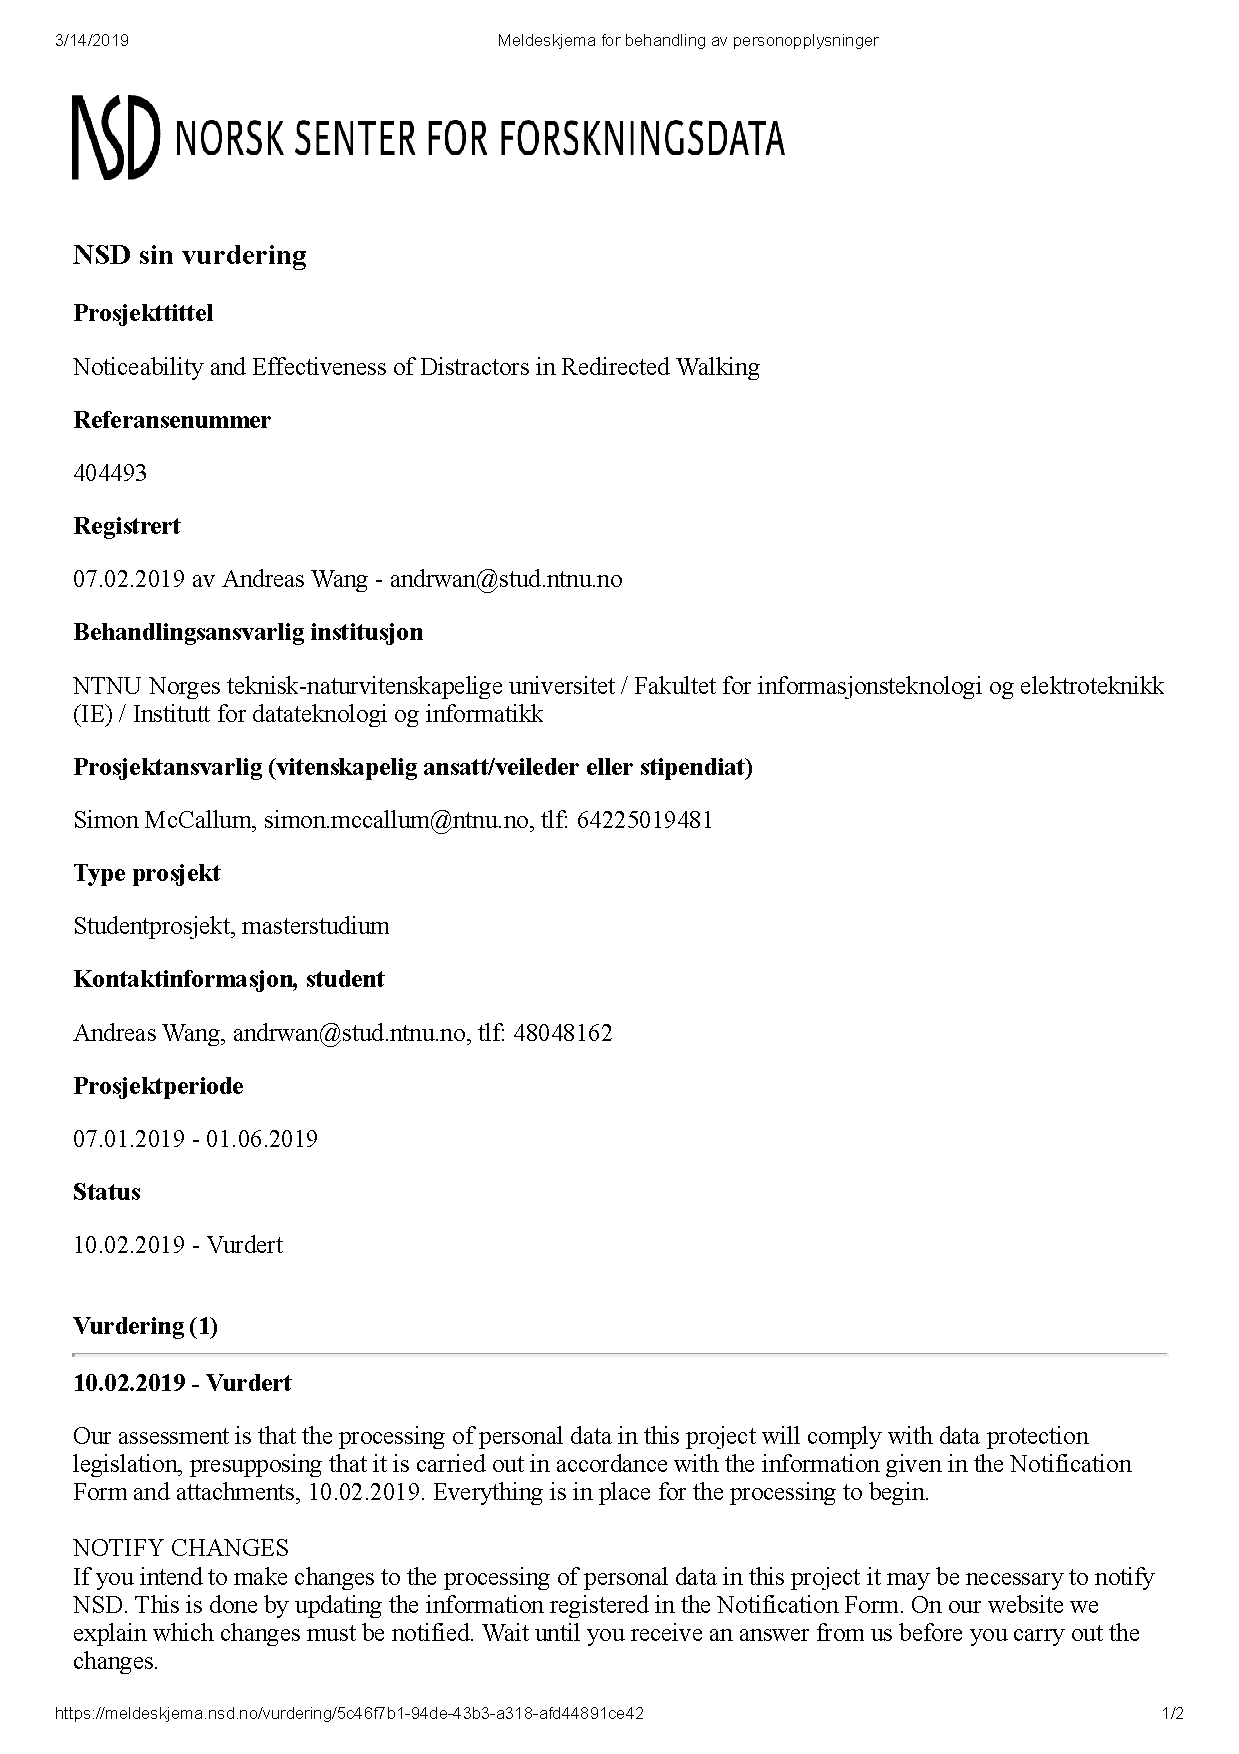
\includepdf[pages=-,pagecommand={},width=\textwidth]{pdfs/NSDApproval.pdf}

\end{document}
